%%
%% This is file `sample-manuscript.tex',
%% generated with the docstrip utility.
%%
%% The original source files were:
%%
%% samples.dtx  (with options: `all,proceedings,bibtex,manuscript')
%% 
%% IMPORTANT NOTICE:
%% 
%% For the copyright see the source file.
%% 
%% Any modified versions of this file must be renamed
%% with new filenames distinct from sample-manuscript.tex.
%% 
%% For distribution of the original source see the terms
%% for copying and modification in the file samples.dtx.
%% 
%% This generated file may be distributed as long as the
%% original source files, as listed above, are part of the
%% same distribution. (The sources need not necessarily be
%% in the same archive or directory.)
%%
%%
%% Commands for TeXCount
%TC:macro \cite [option:text,text]
%TC:macro \citep [option:text,text]
%TC:macro \citet [option:text,text]
%TC:envir table 0 1
%TC:envir table* 0 1
%TC:envir tabular [ignore] word
%TC:envir displaymath 0 word
%TC:envir math 0 word
%TC:envir comment 0 0
%%
%%
%% The first command in your LaTeX source must be the \documentclass
%% command.
%%
%% For submission and review of your manuscript please change the
%% command to \documentclass[manuscript, screen, review]{acmart}.
%%
%% When submitting camera ready or to TAPS, please change the command
%% to \documentclass[sigconf]{acmart} or whichever template is required
%% for your publication.
%%
%%
\documentclass[manuscript,screen]{acmart}

%%
%% \BibTeX command to typeset BibTeX logo in the docs
\AtBeginDocument{%
  \providecommand\BibTeX{{%
    Bib\TeX}}}

%% Rights management information.  This information is sent to you
%% when you complete the rights form.  These commands have SAMPLE
%% values in them; it is your responsibility as an author to replace
%% the commands and values with those provided to you when you
%% complete the rights form.
\setcopyright{acmlicensed}
\copyrightyear{2018}
\acmYear{2024}
\acmDOI{XXXXXXX.XXXXXXX}

%% These commands are for a PROCEEDINGS abstract or paper.
\acmConference[Conference acronym 'XX]{Make sure to enter the correct
  conference title from your rights confirmation emai}{June 03--05,
  2018}{Woodstock, NY}
%%
%%  Uncomment \acmBooktitle if the title of the proceedings is different
%%  from ``Proceedings of ...''!
%%
%%\acmBooktitle{Woodstock '18: ACM Symposium on Neural Gaze Detection,
%%  June 03--05, 2018, Woodstock, NY}
\acmISBN{978-1-4503-XXXX-X/18/06}

\usepackage{tcolorbox}
\usepackage{pdflscape}
\newcommand{\loss}{\mathcal{L}}
\newcommand{\labels}{L}
\newcommand{\features}{\mathcal{Y}}
\usepackage{balance}
\usepackage{cleveref}
\usepackage{subcaption}
\raggedbottom
% \flushbottom
\newcommand{\E}{\mathrm{E}}
\usepackage[section]{placeins}
\usepackage{soul}
\usepackage{tabularx}
\usepackage{multirow}
\newcolumntype{Y}{>{\raggedleft\arraybackslash}X}
\newcolumntype{Z}{>{\centering\arraybackslash}X}
\usepackage{listings}
\usepackage{algorithm}
\usepackage{algorithmic}
\usepackage{afterpage}
\usepackage{hyperref}
\usepackage{makecell}
\let\Bbbk\relax
\usepackage{amssymb}

%%

%%
%% Submission ID.
%% Use this when submitting an article to a sponsored event. You'll
%% receive a unique submission ID from the organizers
%% of the event, and this ID should be used as the parameter to this command.
%%\acmSubmissionID{123-A56-BU3}

%%
%% For managing citations, it is recommended to use bibliography
%% files in BibTeX format.
%%
%% You can then either use BibTeX with the ACM-Reference-Format style,
%% or BibLaTeX with the acmnumeric or acmauthoryear sytles, that include
%% support for advanced citation of software artefact from the
%% biblatex-software package, also separately available on CTAN.
%%
%% Look at the sample-*-biblatex.tex files for templates showcasing
%% the biblatex styles.
%%

%%
%% The majority of ACM publications use numbered citations and
%% references.  The command \citestyle{authoryear} switches to the
%% "author year" style.
%%
%% If you are preparing content for an event
%% sponsored by ACM SIGGRAPH, you must use the "author year" style of
%% citations and references.
%% Uncommenting
%% the next command will enable that style.
%%\citestyle{acmauthoryear}


%%
%% end of the preamble, start of the body of the document source.
\begin{document}

%%
%% The "title" command has an optional parameter,
%% allowing the author to define a "short title" to be used in page headers.
\title{Learning to Associate: Multimodal Inference with Fully Missing Modality Data}

%%
%% The "author" command and its associated commands are used to define
%% the authors and their affiliations.
%% Of note is the shared affiliation of the first two authors, and the
%% "authornote" and "authornotemark" commands
%% used to denote shared contribution to the research.
\author{Jack Geraghty}
\email{jack.geraghty@ucdconnect.ie}
\orcid{0000-0002-5544-9484}
\affiliation{%
  \institution{School of Computer Science, University College Dublin}
  \streetaddress{D04W1W8}
  \city{Dublin}
  \state{Dublin} 
  \country{Ireland}
  \postcode{D04W1W8}
}

\author{Andrew Hines}
\email{andrew.hines@ucd.ie}
\orcid{0000-0001-9636-2556}
\affiliation{%
  \institution{School of Computer Science, University College Dublin}
  \streetaddress{D04W1W8}
  \city{Dublin}
  \state{Dublin}
  \country{Ireland}
  \postcode{D04W1W8}
}

\author{Fatemeh Golpayegani}
\email{fatemeh.golpayegani@ucd.ie}
\orcid{0000-0002-3712-6550}
\affiliation{%
  \institution{School of Computer Science, University College Dublin}
  \streetaddress{D04W1W8}
  \city{Dublin}
  \state{Dublin}
  \country{Ireland}
  \postcode{D04W1W8}
}


%%
%% By default, the full list of authors will be used in the page
%% headers. Often, this list is too long, and will overlap
%% other information printed in the page headers. This command allows
%% the author to define a more concise list
%% of authors' names for this purpose.
% \renewcommand{\shortauthors}{Geraghty et al.}


\begin{abstract}
In this paper, we propose \textbf{Cross-Modal Association Models (C-MAMs)}, a novel approach for handling missing modalities during inference in multimodal learning. 
Unlike existing methods that modify the training process, C-MAMs generate missing modality features \textbf{post-training}, preserving the integrity of the original multimodal model. 
In this paper, we: \textbf{(i)} formalise the problem of missing modality inference and its challenges, \textbf{(ii)} introduce C-MAMs as a flexible, lightweight, post-hoc solution for reconstructing missing modality embeddings, \textbf{(iii)} evaluate their effectiveness across diverse datasets, tasks, and baseline models, and \textbf{(iv)} analyze the quality of the generated versus the ground-truth features to quantify the reconstruction fidelity. 
Experimental results show that C-MAMs \textbf{significantly mitigate performance degradation} due to missing modalities, in some cases fully restoring baseline performance, even when \textbf{trained on 10\%} of the data. 
We conclude that post-training feature reconstruction is an effective, targeted alternative to existing methods, with broad applicability in multimodal systems.
\end{abstract}


%%
%% The code below is generated by the tool at http://dl.acm.org/ccs.cfm.
%% Please copy and paste the code instead of the example below.
%%
\begin{CCSXML}
<ccs2012>
   <concept>
       <concept_id>10003752.10010070.10010071</concept_id>
       <concept_desc>Theory of computation~Machine learning theory</concept_desc>
       <concept_significance>500</concept_significance>
       </concept>
   <concept>
       <concept_id>10010147.10010257.10010293.10010319</concept_id>
       <concept_desc>Computing methodologies~Learning latent representations</concept_desc>
       <concept_significance>500</concept_significance>
       </concept>
   <concept>
       <concept_id>10010147.10010257.10010258.10010259.10010263</concept_id>
       <concept_desc>Computing methodologies~Supervised learning by classification</concept_desc>
       <concept_significance>300</concept_significance>
    </concept>
    <concept>
        <concept_id>10003752.10010070.10010071.10010289</concept_id>
        <concept_desc>Theory of computation~Semi-supervised learning</concept_desc>
        <concept_significance>300</concept_significance>
    </concept>
    <concept>
        <concept_id>10010147.10010257.10010258.10010259.10010264</concept_id>
        <concept_desc>Computing methodologies~Supervised learning by regression</concept_desc>
        <concept_significance>300</concept_significance>
    </concept>
</ccs2012>
\end{CCSXML}

\ccsdesc[500]{Theory of computation~Machine learning theory}
\ccsdesc[500]{Computing methodologies~Learning latent representations}

\ccsdesc[300]{Computing methodologies~Supervised learning by classification}
\ccsdesc[300]{Computing methodologies~Supervised learning by regression}
\ccsdesc[300]{Computing methodologies~Supervised learning by regression}





%%
%% Keywords. The author(s) should pick words that accurately describe
%% the work being presented. Separate the keywords with commas.
\keywords{multimodal machine learning, cross-modal learning, cross-modal perceptual association, missing data, imbalanced modality information}


% %%
% %% This command processes the author and affiliation and title
% %% information and builds the first part of the formatted document.
\maketitle

\section{Introduction}\label{sec:intro}

Multimodal machine learning,
which integrates diverse data types
such as audio, video, text, and sensor readings,
has significantly advanced applications
in autonomous systems, healthcare, human-computer interaction,
and smart environments~\cite{He2024Multimodal,Chen2023Dialog,Ang2024Temporal,Wang2023Customer,Hu2021Identifying,Bano2024FedCMD,Yin2023Hybrid,zhao-etal-2021-missing,redcore}.
While the ability to leverage multiple modalities enhances predictive performance and robustness,
real-world deployment often faces critical challenges
with missing modality data,
particularly in safety-sensitive and resource-constrained environments.
In autonomous driving and distributed IoT networks,
for instance,
models must maintain reliable performance
despite incomplete or degraded inputs,
making robust handling of missing modalities
essential for practical deployments.
Missing modality data manifests in two forms:
\emph{partially missing},
where fragments of a modality are lost, for example, missing words in a sentence,
and \emph{fully missing},
where an entire modality becomes unavailable,
for example, complete sensor failure.
The latter presents a substantial challenge,
as standard multimodal models
typically depend on the joint availability of modalities
for accurate predictions.
During inference,
missing modalities can significantly degrade performance,
particularly when different modalities
contribute unequally to the decision-making process.
This degradation is especially problematic
in real-world applications
where retraining models or maintaining multiple variants
is often infeasible due to computational and deployment constraints.

Understanding how modalities interact
is crucial for effective missing modality reconstruction.
As illustrated in Figure~\ref{fig:info_types},
modalities can share \emph{mutual information}
that reinforces predictions,
provide \emph{complementary information}
unique to each modality,
exhibit \emph{contrastive relationships}
that may introduce conflicting signals,
or demonstrate \emph{imbalanced contributions}
where one modality dominates others~\cite{%
	wang2020makes,Peng2022Balanced,%
	hazarika2022analyzing,geraghty2023understanding,redcore}.
These interaction patterns influence how effectively
missing modality data can be reconstructed,
particularly when leveraging remaining modalities
to generate missing features.
\begin{figure}[b!]
    \centering
    \begin{subfigure}[b]{0.24\textwidth}
        \centering
        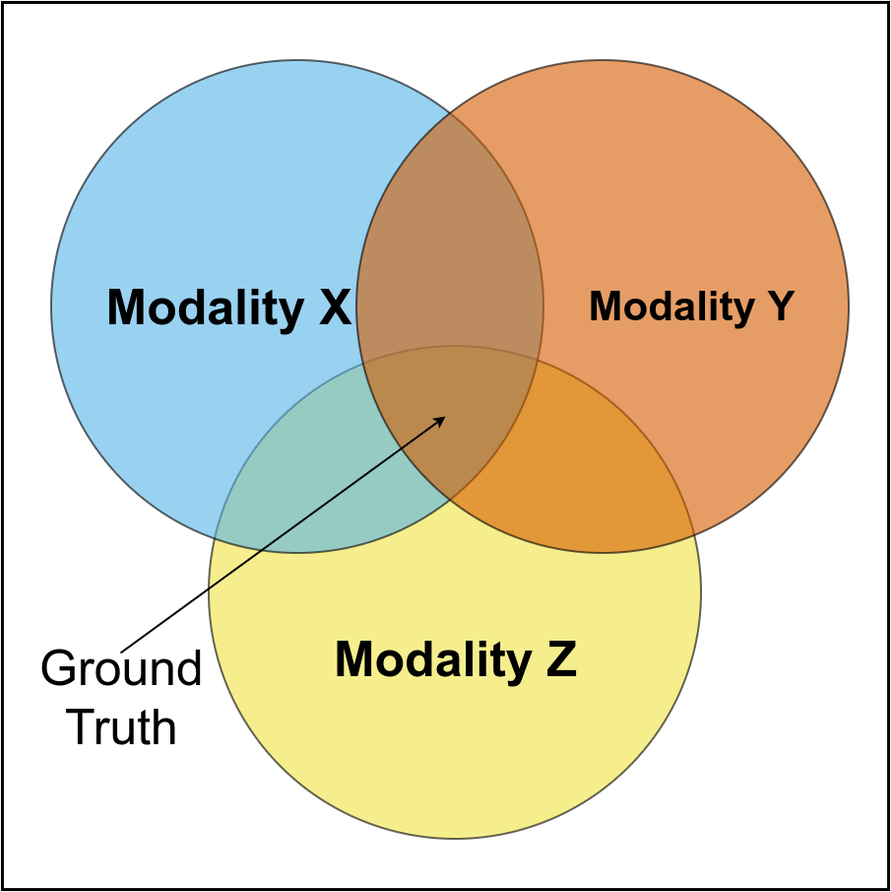
\includegraphics[height=1in]{imgs/mutual_info.png}
        \caption{Mutual Information}
        \label{fig:mutual}
    \end{subfigure}
    \hfill
    \begin{subfigure}[b]{0.24\textwidth}
        \centering
        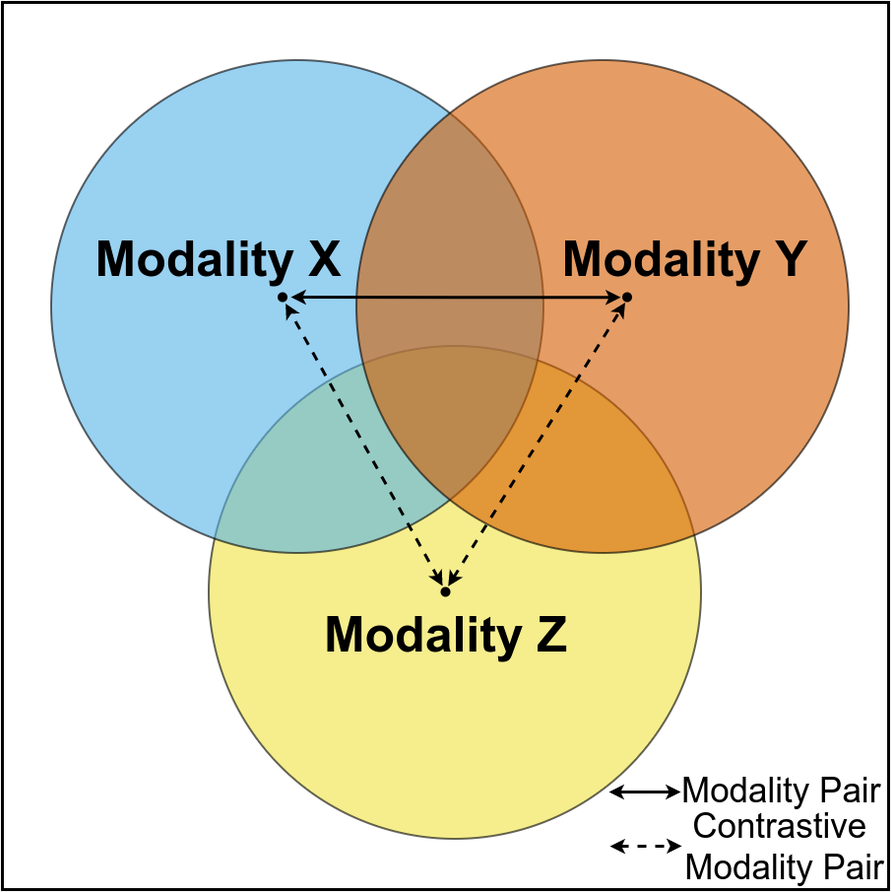
\includegraphics[height=1in]{imgs/complementary_info.png}
        \caption{Complementary Information}
        \label{fig:complementary}
    \end{subfigure}
    \hfill
    \begin{subfigure}[b]{0.24\textwidth}
        \centering
        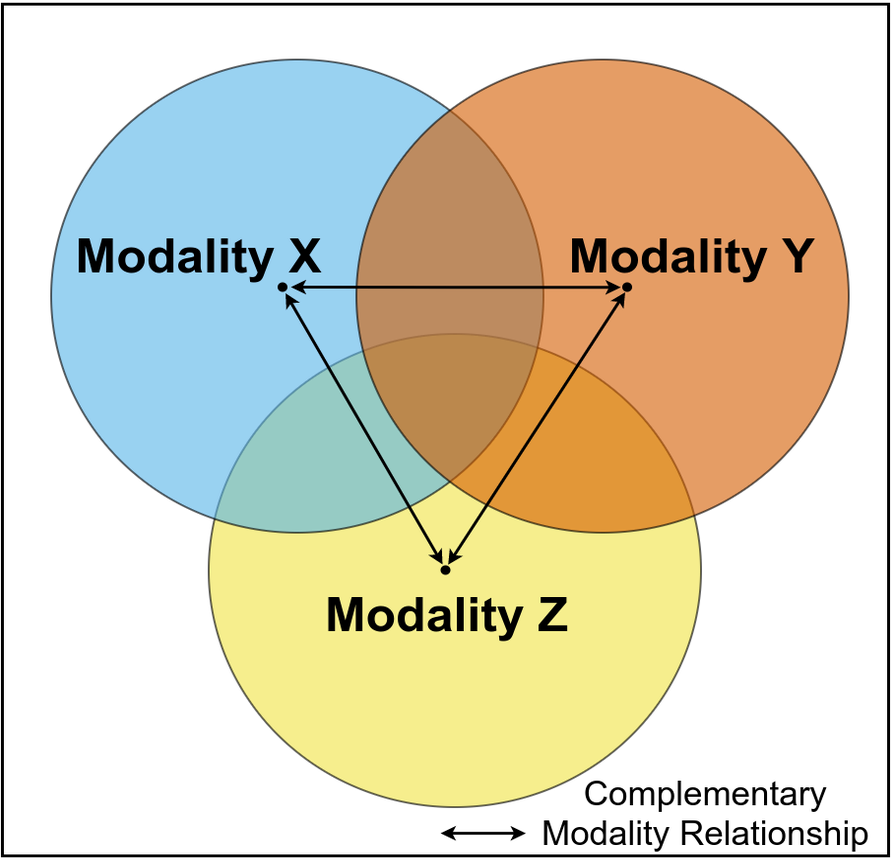
\includegraphics[height=1in]{imgs/contrastive_info.png}
        \caption{Contrastive Information}
        \label{fig:contrastive}
    \end{subfigure}
    \hfill
    \begin{subfigure}[b]{0.24\textwidth}
        \centering
        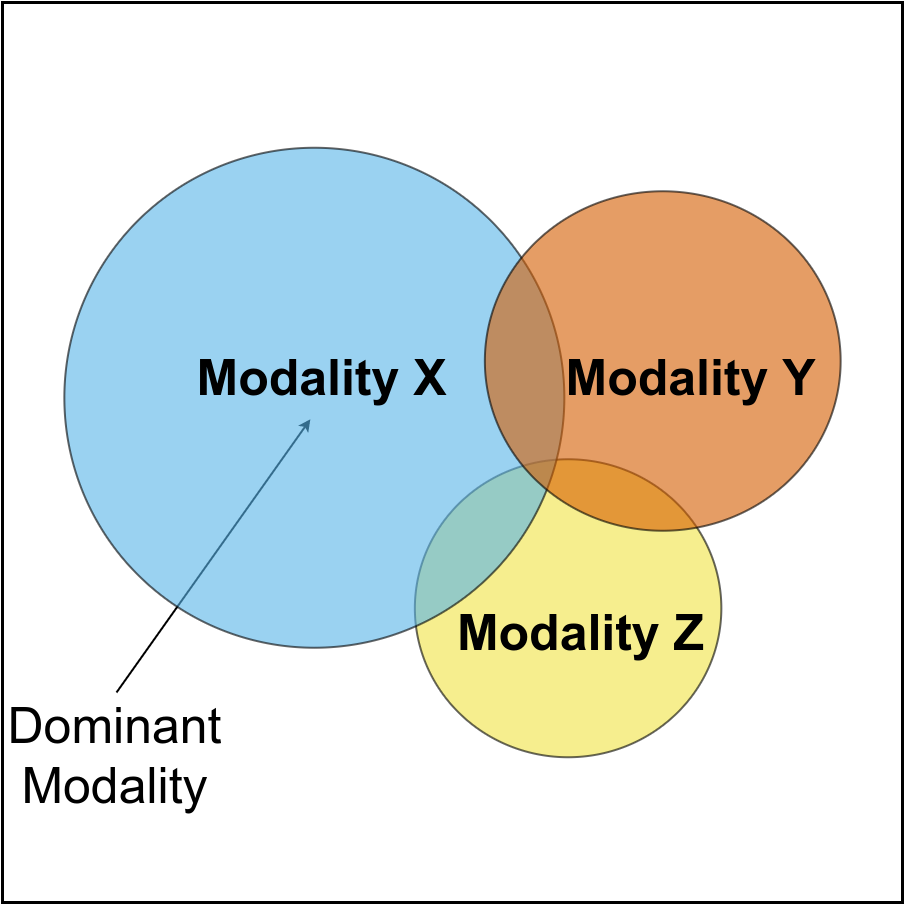
\includegraphics[height=1in]{imgs/imbalanced_info.png}
        \caption{Imbalanced Information}
        \label{fig:imbalanced}
    \end{subfigure}
    
    \caption{%
        Types of information interactions between modalities. 
        \textbf{(a)} Mutual information: Shared knowledge between modalities reinforces predictions.
        \textbf{(b)} Complementary information: Unique knowledge from each modality contributes to the overall task.
        \textbf{(c)} Contrastive information: Modalities provide conflicting signals, which may challenge fusion.
        \textbf{(d)} Imbalanced information: One modality dominates, suppressing the contribution of others.
        Understanding these relationships is critical for effective multimodal learning, particularly when handling missing modalities.
    }
    \label{fig:info_types}
    \Description{Types of information interactions between modalities. 
        \textbf{(a)} Mutual information: Shared knowledge between modalities reinforces predictions.
        \textbf{(b)} Complementary information: Unique knowledge from each modality contributes to the overall task.
        \textbf{(c)} Contrastive information: Modalities provide conflicting signals, which may challenge fusion.
        \textbf{(d)} Imbalanced information: One modality dominates, suppressing the contribution of others.
        Understanding these relationships is critical for effective multimodal learning, particularly when handling missing modalities.}
\end{figure}

Existing approaches for handling missing modalities
primarily intervene during training,
either through generative methods
that learn joint distributions
over modalities~\cite{10.1145/3394486.3403182,YUAN2012622,10.1007/978-3-031-30675-4_19,9755996,Tran_2017_CVPR,8253467,9258396,smil,10.1145/3219819.3219963,10.1145/3474085.3475585,zhao-etal-2021-missing,wei2022perception,10.1145/3581783.3611696}
or non-generative techniques
that train models to be robust to missing samples~\cite{%
	ma2021maximum,Matsuura_2018_ECCV_Workshops,10.1145/3394486.3403234,7993002,QIAN2023443,hazarika2022analyzing}.
However,
these methods often require complex architectural modifications
or introduce additional training constraints,
making them challenging to integrate
with existing deployed systems.
Moreover,
they typically do not address
the practical challenge of handling
fully missing modalities during inference
without modifying the base model.

In this paper,
we propose \textbf{Cross-Modal Association Models (C-MAMs)},
a simple yet effective post-training solution
for handling fully missing modality data at inference time.
Unlike existing approaches,
C-MAMs operate independently of the base multimodal model,
preserving its structure and learned representations
while providing flexible reconstruction capabilities
when needed.
This modular design enables C-MAMs
to be selectively deployed
without disrupting existing systems,
making them particularly suitable
for distributed and resource-constrained environments.

Our approach builds on two key premises.
First,
we leverage multimodal models
trained on complete data
to ensure optimal modality-specific representations.
Second,
we demonstrate that the remaining modalities
contain sufficient information
to generate embeddings that significantly improve
inference performance compared to the missing modality conditions.
Through extensive experimentation,
we show that these reconstructed embeddings
can restore performance close to baseline levels
using a straightforward architecture
and standard mean squared error loss,
challenging the assumption that complex solutions
are necessary for effective missing modality handling.

\textbf{The key contributions of this work are as follows:}
\begin{enumerate}
	\item \textbf{We introduce Cross-Modal Association Models (C-MAMs)},
	a modular post-training solution that effectively reconstructs
	missing modality embeddings through simple association networks,
	achieving significant performance improvements
	without modifying the original multimodal model.
	\item \textbf{We demonstrate through comprehensive statistical analysis}
	that C-MAMs can effectively reconstruct missing modality embeddings
	even with imperfect latent space alignment,
	revealing important insights about embedding reconstruction requirements.
	\item \textbf{We validate through extensive empirical evaluation}
	that C-MAMs consistently improve inference-time performance
	across multiple datasets and architectures,
	with improvements of up to 39\% in missing modality scenarios, and be trained to a similar level of performance on a much smaller subset of the original data.
	\item \textbf{We establish C-MAMs as a practical foundation}
	for robust multimodal deployment in distributed environments,
	providing a flexible solution that balances
	implementation simplicity with effective performance recovery.
\end{enumerate}

\section{Related Works - Handling Missing Modalities}\label{sec:related_works}

The following paragraphs provide details on handling partially missing modality data and generative and non-generative approaches to fully missing modality data. This section focuses on methods of handling missing modality data, we provide the related works that motivated C-MAMs in \Cref{sec:proposed_method}.

\textbf{Handling of Partially Missing Data}: Data loss is often partial, where corrupted or missing portions can impact model training efficacy. Several methods address this challenge. \citet{8273601} propose a multimodal autoencoder (MMAE) trained on complete data before randomly masking a modality to encourage cross-modal learning. Other approaches reconstruct missing data at the modality level, such as \citet{10.1007/978-3-030-03493-1_62}, who use a Cartesian Genetic Programming and Recurrent Neural Network (CGPRNN) with a sliding window to leverage RNN memory for signal restoration. Building on \cite{8273601}, \citet{NIPS2012_6cdd60ea} and \citet{9099281} employ stacked denoising autoencoders with white Gaussian noise to corrupt samples, evaluating their method by removing overlaid text from images.

Simpler methods involve discarding incomplete samples or padding missing data with zeros or averages \cite{10.1145/3395035.3425202, ma2021maximum, 9258396}. While effective, these methods do not preserve inter-modal correlations. \citet{10122560} propose the Efficient Multimodal Transformer with Dual Level Feature Restoration (EMT-DLFR), which integrates a transformer with a reconstruction network to generate missing sequences. EMT-DLFR improves over prior methods by reducing quadratic scaling costs and enhancing overall performance. Notably, when the percentage of missing data reaches 100\%, it effectively addresses the fully missing data problem.

Other studies leverage cross-modal signals for reconstruction. \citet{9563268} introduce an audio-driven GAN model that aligns audio with available video frames to restore missing video content. \citet{9842374} present an audio-haptic fused visual signal restoration (AHFVR) approach, employing semantic fusion of audio and haptic features, adversarial mapping to a shared latent space, and hierarchical knowledge distillation to enhance visual reconstruction. AHFVR demonstrates superior performance over single-modality and non-hierarchical methods in both benchmark datasets and real-world scenarios.

\textbf{Handling of Fully Missing Data - Non-generative Methods}: These approaches incorporate missing modality data into the training procedure of multimodal models. The intuition with these approaches is that if a model is given samples with missing data during training, it will be more capable of dealing with missing data during inference. \citet{10.1145/3394486.3403234} utilise a knowledge distillation framework for handling incomplete modalities. First, unimodal teacher models are trained using all available samples, including those with missing data. Then, the multimodal student network is trained using complete samples and the output of the teacher models. \citet{7993002}  propose a multi-hypergraph learning approach for handling incomplete data. The hypergraph model is trained on all modality data, whether it contains missing data or not. The authors do not report the degree of missing data; they only record what is recorded in the base dataset itself. \citet{ma2021maximum} propose a maximum likelihood-based approach that characterises the conditional distribution of the modality-complete data and the modality-missing data. The authors develop a generalised softmax function to implement the likelihood estimation efficiently. In this approach, missing data is handled during training. \citet{Matsuura_2018_ECCV_Workshops} propose a Bayesian Canonical correlation-based approach which estimates the relationships among the non-missing data and the feature space in the non-missing modality. Missing data is incorporated into the model's training via the likelihood function. \citet{QIAN2023443} uses contrastive learning and GAN augmentation to handle incomplete modality data. The GAN aspect of the model is not used to generate data for inference but to provide a balance of positive and negative pairs for contrastive learning. 

\textbf{Handling of Fully Missing Data - Generative Methods}:
These methods all reconstruct the missing modality data in some way, for example, full imputation of the missing modality or weight reconstruction. \citet{9755996} propose a UU-net autoencoder architecture to generate the missing modality. The first U-net handles intramodal fusion, while the second handles intermodal fusion. The purpose of the two networks is first to obtain unique feature representation and, secondly, to learn a shared latent space. Missing modalities are then generated by minimising the reconstruction error across both U-nets. Missing data is handled during the training process. \citet{Tran_2017_CVPR} propose a stacked residual autoencoder approach named Cascading Residual Autoencoder (CRA).
The approach is similar to those proposed in \cite{8273601,9099281}, except the denoising autoencoders are replaced with residual ones. Residual autoencoders output the difference between the input and output data rather than generating just the output. Then, the estimation is refined at each layer by stacking these residual autoencoders. The missing data is handled during training. A graph-based approach is proposed by \citet{10.1007/978-3-031-30675-4_19}. The authors construct a bipartite graph where samples and modalities are two types of nodes, and edges represent the observed modality value. Once the initial graph model is trained, it can be further trained to impute edge values for missing modalities. The model handles missing data during the training phase. \citet{YUAN2012622} propose a hybrid approach to handling missing data. They develop a multi-source feature learning model that learns a common feature space for the available modalities. They then use other imputation approaches (zeroing/averaging, k-nearest neighbours, singular value decomposition and expectation maximisation) alongside ensemble learning to perform decision-level fusion. \citet{smil} propose a weight-learning approach to generating missing modality data. The approach leverages Bayesian meta-learning to achieve both flexibility and efficiency. Missing modalities are approximated using a weighted sum of modality priors instead of directly generating the missing modality. This method approaches the problem of missing data during training. \citet{10.1145/3474085.3475585} propose a transformer-based feature reconstruction network. The network is trained to transform partially or entirely missing modality features into complete modalities. Complementary modality information is used to enhance the missing data under the guidance of the reconstruction loss. The transformation uses an attention mechanism to attend to the input modalities' missing portions. \citet{10.1145/3394486.3403182} propose a graph-based fusion method to enable learning on incomplete multimodal data. They construct a heterogeneous hypernode graph to model combinations of complete and incomplete modalities. The technique sees promising results without the need to impute modalities. \citet{8253467} propose a method which aims to exploit both semantic complementarity and similar distributions (the authors assume that modalities share identical distributions). To achieve this, they utilise a two-step process where an Isomorphic Linear Correlation Analysis (ILCA) is performed first. Then, this is followed by Identical Distribution Pursuit Completion to impute the missing data. \citet{10.1145/3219819.3219963} propose a deep adversarial learning approach which generates missing modalities. The authors formulate the problem as a conditional image generation task, using a GAN and an auxiliary adversarial loss function to generate high-quality missing modality images. Cross-partial multi-view networks (CPM-Nets) \cite{9258396} also utilise a GAN to impute missing information views. The network is trained to create a unified latent space, which is then used with the adversarial strategy to reconstruct a missing modality. \citet{10.1145/3581783.3611696} introduces Sample Less Learn More (SLLM), a technique that uses a frame feature restoration module to reconstruct features of deliberately omitted frames during training, thereby reducing computational costs in video action recognition. Unlike methods addressing missing modalities at inference time, SLLM focuses on mitigating performance impacts caused by intentionally reduced training data, achieving significant efficiency gains with minimal accuracy loss across various action recognition frameworks. The Multimodal Imagination Network (MMIN) proposed by \citet{zhao-etal-2021-missing} uses the CRA architecture proposed in \cite{Tran_2017_CVPR} to generate the multimodal embeddings created by the input modalities. They first train a baseline late fusion model, which is then used as a foundation model for the imagination network. They re-train the baseline model with the imagination network now included. The MMIN was evaluated on two datasets, focused on the sole task of multimodal sentiment analysis, and established a strong baseline for generating missing data in multimodal sentiment analysis. 

\textbf{Inference-Time Missing Modality Solutions and Modular Deployment Needs: } Despite extensive research on handling missing modalities during training, relatively few works have addressed inference-time reconstruction. Most approaches assume that models should be trained for robustness to missing data rather than developing methods for post-hoc adaptation. This assumption limits the flexibility of existing techniques, particularly in real-world settings where models may be deployed in environments where re-training is infeasible. Addressing missing modalities at inference time is essential for improving model longevity and adaptability without increasing training complexity.

Furthermore, many existing multimodal learning methods assume centralised computational resources, limiting their applicability in distributed environments such as federated learning, IoT, and multi-agent systems~\cite{NEURIPS2023_9156b0f6,adnan_cfl_2022}. The constraints of these environments necessitate \textbf{modular, targeted solutions} that can function independently of the primary multimodal model. Studies in federated learning have shown that \textbf{heterogeneous modality availability} across clients can hinder performance, requiring solutions that do not rely on centralised data access~\cite{pretrained_multimodal_decision_making_yunhao_24}. Our work addresses these gaps by introducing a \textbf{post-training, inference-time missing modality reconstruction framework} that enables adaptable deployment without requiring modifications to the original model.



\section{Cross-Modal Association Models}
\label{sec:proposed_method}
This section details the missing modality feature generation task using a C-MAM. It is split into three parts: the inspiration behind the approach, a high-level explanation of it, and the mathematical formulation and algorithm of the generation task.

\textbf{Cross-modal perceptual associations} describe the cognitive mechanism where variations in one sensory modality evoke responses in another. This phenomenon influences how multimodal information is processed and integrated~\cite{seeing_what_you_hear,Glicksohn2013,Mondloch2004,Spence2011,HAUW2023167,9018269}. An extreme example is synaesthesia, where individuals automatically associate stimuli from one modality with responses in another, such as perceiving specific colours when hearing certain musical notes. A well-known instance of this perceptual filling-in process is illustrated in the silent film \textit{Steamboat Bill, Jr.}, where viewers can imagine the sound of a collapsing house despite the absence of audio (Figure~\ref{fig:steamboat}).
\begin{figure}[htbp!]
    \centering
    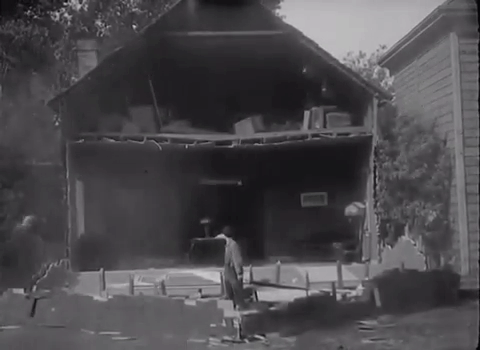
\includegraphics[width=0.25\textwidth]{imgs/steamboat_bill_jr_still.png}
    \caption{The aftermath of the collapsed house. Still taken from the movie [Public Domain] via \href{https://commons.wikimedia.org/wiki/File:GIF_of_Buster_Keaton_in_\%22Steamboat_Bill_Jr\%22_1928.gif}{Wikimedia Commons} }
    \label{fig:steamboat}
\end{figure}

This natural human ability to infer missing sensory information inspires our approach. Similar associations can be learnt within a machine learning framework, allowing a model to infer a missing modality’s features from the remaining available modalities. Rather than modifying or fine-tuning the entire multimodal model, we leverage the pre-trained modality-specific encoders to train a new model, a C-MAM, which generates missing modality embeddings \textbf{without requiring alterations to the original multimodal system.}

\textbf{Learning to Associate} Building on the concept of cross-modal perceptual associations, we apply these ideas to multimodal machine learning. In human perception, different senses interact to compensate for missing information, allowing individuals to infer one sensory input from others. Our approach trains a model to reconstruct missing modality embeddings using the trained encoders of the available modalities, focusing on learning about the model rather than the task being performed by the model.

The proposed \textbf{Cross-Modal Association Models (C-MAMs)} learn associations between available and missing modalities without modifying the multimodal model. Unlike methods that require alterations to the underlying architecture and training procedure, C-MAMs operate \textit{post-hoc}, learning to generate missing modality embeddings from pre-trained encoder outputs. This ensures the trained multimodal model remains unchanged and that C-MAMs are used only when a modality is missing.


\subsection{Problem Formulation}
Multimodal learning improves prediction performance by leveraging multiple data sources like audio, video, and text. However, real-world scenarios often introduce the challenge of \textbf{missing modalities at inference time}, which can significantly degrade model performance. Our objective is to \textbf{reconstruct missing modality embeddings at inference time without modifying the original multimodal model}, ensuring robustness to missing data.

\textbf{Multimodal Learning Framework:} A multimodal dataset consists of $N$ samples, each containing $K$ modalities. Let $M = \{m_1, \dots, m_K\}$ denote the set of input modalities, and let $D = \{(d_1, y_1), \dots, (d_N, y_N)\}$ be the dataset, where each $d_i = \{m_{1_i}, \dots, m_{K_i}\}$ represents the observed modalities, and $y_i \in L$ is the target label. A multimodal model $MM$ learns feature representations through modality-specific encoders $E_m$, $E(d) \mapsto \{f_{m_1}, \dots, f_{m_K}\}, \quad f_{m_i} \in \mathbb{R}^{k_i}$, and fuses them to make predictions, $C(F(f_{m_1}, \dots, f_{m_K})) \mapsto \hat{y}$, where $C$ is the classifier, and $F$ is a fusion function such as concatenation, averaging, or attention-based fusion. The multimodal model is trained using a supervised loss function $\mathcal{L}$, such as cross-entropy or mean absolute error (MAE): $\{\phi_C^*, \phi_E^*\} = \arg\min_{\phi_C, \phi_E} \mathcal{L}(y, \hat{y})$.

\textbf{Challenges of Missing Modalities:} At inference time, one or more modalities may be entirely absent, leading to incomplete inputs. Let \( M' \subset M \) represent the subset of missing modalities, and let \( S = M \setminus M' \) denote the available modalities. The resulting input to the multimodal model is: $d' = d - M', \quad d' = \{ m_i \mid m_i \in S \}$.
This formulation generalises the missing modality scenario to allow for any combination of absent modalities, rather than assuming only one missing modality. Standard multimodal models are not explicitly designed to handle such cases, often relying on the assumption that all modalities are present during inference. A common approach to handling missing modalities is incorporating a reconstruction module within the classification model. For example, autoencoders trained to reconstruct all modalities while jointly optimising for classification~\cite{zhao-etal-2021-missing,redcore}. In these methods, the model is trained to both \textbf{predict the output and reconstruct modality embeddings}, which introduces \textbf{competing objectives}. This can lead to suboptimal representations, as the model must balance classification and reconstruction. Additionally, these methods require modifying the core multimodal model, making them impractical for already deployed systems where retraining is infeasible.

\subsection{Cross-Modal Association Models (C-MAMs)}
To address these limitations, we introduce \textbf{Cross-Modal Association Models (C-MAMs)}, a targeted and modular approach that reconstructs missing modality embeddings without modifying the trained multimodal model. Unlike existing approaches, C-MAMs are \textbf{fully decoupled} from the multimodal model, ensuring that reconstruction does not interfere with classification.

C-MAMs reconstruct missing modality embeddings by leveraging the available modalities' feature representations. Given a missing modality $m'$, the remaining available modalities $S = M \setminus \{m'\}$ are processed through their trained encoders $\tilde{E}$, and the extracted features are mapped to the missing modality’s feature space via an association network $A$:
\begin{equation*}
\hat{f}_{m'} = A(f_S) = W f_S + b
\end{equation*}
where $f_S$ is the fused embedding from available modalities, and $W, b$ are learnable parameters. A C-MAM is only trained to reconstruct the missing embedings of a single modality. Multiple C-MAMs can be trained for different missing modalities, allowing the multimodal model to handle any combination of missing modalities.~\footnote{Multiple C-MAMs could be jointly optimised to improve the reconstruction of missing modalities in a given model, potentially resulting in improved results compared to reconstructing each modality independently. However, we leave this as future work since and instead focus on reconstructing a single missing modality at a time to better isolate and study the core problem of modality reconstruction.}



\textbf{Training and Integration:} C-MAMs are trained \textbf{post-hoc} using the learnt feature representations of a pre-trained multimodal model. The objective is to minimise the reconstruction loss between the predicted missing modality embedding $\hat{f}_{m'}$ and the ground-truth embedding $f_{m'}$: $\{\phi_{\tilde{E}}^*, \phi_{A}^*\} = \arg\min_{\phi_{\tilde{E}}, \phi_{A}} \mathcal{L}_{MSE}(f_{m'}, \hat{f}_{m'})$
% \end{equation*}
where $\mathcal{L}_{MSE}$ is the MSE loss~\footnote{MSE is chosen for its simplicity and effectiveness in feature reconstruction, avoiding unnecessary complexity.}. At inference time, the trained C-MAM reconstructs the missing modality embedding, which is then passed to the classifier:
\begin{equation*}
\boxed{
C(F(E(d') \oplus A(\tilde{E}(d')))) \mapsto \hat{y}
}
\end{equation*}
This allows the multimodal model to function as if no modality were missing, without requiring retraining or modifications to its original architecture.

\textbf{Architecture and Training Process:} Figure~\ref{fig:ACM_TOMM_MM_CMAM_ARCH} illustrates the \textbf{C-MAM architecture} integrated into a multimodal model. The \textbf{left side} shows a standard multimodal model with modality-specific encoders, fusion, and classification. The \textbf{middle} depicts C-MAM training, where a missing modality is reconstructed from available ones and trained using MSE loss against ground-truth embeddings. The \textbf{right side} shows the trained C-MAM reconstructing missing modalities during inference. The training process, detailed in Algorithm~\ref{alg:cmam_training}, first trains the multimodal model for classification, then uses its embeddings as ground-truth to train the C-MAM. This design keeps classification and reconstruction \textbf{decoupled}, with reconstruction dependent on the classification model's representations but not vice versa.


\section{Experimental Setup}
\label{sec:experiments}
The following sections detail experiments evaluating our proposed C-MAM approach. We start with toy datasets and simple multimodal models to establish a proof-of-concept. Next, we increase complexity by incorporating more data, modalities, and challenging classification tasks. Finally, we compare C-MAM against two state-of-the-art methods for missing modality data, EMT-DLFR for partially missing data and MMIN for fully missing data. Additionally, we assess performance under varying missing data percentages to understand how multimodal models leverage information from different modalities. Our evaluation spans six multimodal models across eight datasets with four modalities.
\begin{figure}[ht!]
    \centering
    \includegraphics[width=0.99\textwidth]{imgs/C-MAM Architecture.pdf}
    \caption{C-MAM architecture and integration. The left side shows a standard multimodal model with modality-specific encoders, fusion, and classification. The middle illustrates a C-MAM for a missing modality case, where Modality C is reconstructed using A and B and compared against the ground-truth embedding with MSE. The right side demonstrates the integration of the trained C-MAM into the multimodal model, enabling inference-time reconstruction of missing modalities.}
    \label{fig:ACM_TOMM_MM_CMAM_ARCH}
\end{figure}
\begin{algorithm}[ht!]
    \small
\caption{Training Multimodal Model and C-MAM}
\label{alg:cmam_training}
\begin{algorithmic}[1]
\REQUIRE Dataset $D$, Multimodal Model $MM$, Missing modality $m'$, Available modality set $S$, Loss function $\mathcal{L}_{MAE}$

\FOR{epoch $= 1$ to $\text{num\_epochs\_MM}$}
\FOR{$(d_j, y_j) \in D$}
\STATE Compute modality embeddings $f_j = (E_1(m_{1j}), \dots, E_K(m_{Kj}))$
\STATE Compute fused representation $f_{fused} = F(f_j)$
\STATE Predict $\hat{y}_j = C(f_{fused})$
\STATE Compute loss: $\text{Loss}_{MM} = \mathcal{L}(y_j, \hat{y}_j)$
\STATE Update multimodal model
\ENDFOR
\ENDFOR

\STATE Initialise C-MAM with encoders $\tilde{E}$ and association network $A$

\FOR{epoch $= 1$ to $\text{num\_epochs\_CMAM}$}
\FOR{$(d_j, y_j) \in D$}
\STATE Compute target embedding $f_{m'} = E_{m'}^*(m_{m'j})$
\STATE Compute available embeddings $f_S = F(\{\tilde{E}_i(m_{ij}) | i \in S\})$
\STATE Predict missing modality embedding $\hat{f}_{m'} = A(f_S)$
\STATE Compute loss: $\text{Loss} = \mathcal{L}_{MAE}(f_{m'}, \hat{f}_{m'})$
\STATE Update C-MAM parameters
\ENDFOR
\ENDFOR
\RETURN Optimised $MM^*$ and C-MAM
\end{algorithmic}
\end{algorithm}
\subsection{Experiment 1: \textit{Toy} datasets}


\noindent \textbf{Experiment One} aims to assess the viability of our proposed approach using two datasets: a subset of AudioSet \cite{audioset} and AVMNIST \cite{vielzeuf2018centralnet}, a multimodal extension of the MNIST dataset.

\textbf{AudioSet}: The full AudioSet dataset comprises over 2M, 10s YouTube videos labeled with 632 audio event classes. For our purposes, we selected a subset focusing on entries labeled as containing speech, treating the absence of a speech label as indicative of non-speech. While we initially aimed for 10,000 entries, issues such as copyright notices and unavailable videos resulted in a final dataset of 7,276 entries, with a class imbalance of 61/39 in favor of the speech label. The subset was split into train, validation, and test sets (70-20-10). The \textbf{AudioSet Model} includes a video representation network using a pre-trained and frozen ResNet50 backbone \cite{7780459} followed by a linear layer, and an audio representation network composed of a convolution block (two stacked convolutional layers) and a linear layer. These unimodal features are fused and passed through three linear layers.

\textbf{AVMNIST}: AVMNIST is a multimodal extension of MNIST that includes audio clips of 60 speakers pronouncing digits, resulting in 70k entries. Each image is associated with a randomly (but balanced) selected speaker. Before training, images undergo Gaussian blur, random color inversion, random horizontal flip, and random vertical flip, while audio recordings are converted into Mel-Spectrograms. The dataset, containing ten classes, is split into train, validation, and test sets (70-20-10). The \textbf{AVMNIST Model} consists of an image representation network with two convolution blocks followed by max pooling and two linear layers, and an audio representation network with two convolution blocks with max pooling and one linear layer. The outputs of these networks are fused before being processed by three linear layers.

\subsection{Experiment 2: Advanced datasets}
\textbf{Experiment two} then aims to determine the approach's effectiveness on a more challenging set of tasks with some more modalities. Two more datasets were selected to test the C-MAM approach; a subset of the Kinetics dataset \cite{kinetics}, Kinetics-Sounds \cite{kinetics_sounds} and the MM-IMDb \cite{arevalo2017gated} movie genre classification dataset. 

\textbf{Kinetics-Sounds}: The Kinetics-Sounds dataset is a subset of the Kinetics dataset. It contains 19K 10-second clips, which were obtained by filtering the Kinetics dataset for human action classes that potentially manifest both visually and aurally, for example, "playing the guitar" and "laughing". The videos in the dataset were pre-processed by centre-cropping, normalisation, and uniform random frame selection (eight frames were sampled), and finally converted to a $400x1$ feature tensor by passing it to a pre-trained ResNet50 model. The dataset contains 26 classes and was split into a 70-20-10 train-validation-test split. \textbf{Kinetics-Sounds Model}: The Kinetics-Sounds video representation network uses a ResNet50 backbone network (pre-trained and frozen), followed by two linear layers. The audio representation network consists of three convolution blocks with average pooling after each block, followed by two linear layers. The multimodal model then consists of a fusion layer and two linear layers.

\textbf{MM-IMDb}: The MM-IMDb dataset contains two modalities: images and text. The data is taken from the IMDB\footnote{https://www.imdb.com} website. Each entry in the dataset includes a description of the movie, a promotional poster of the film and a set of genres associated with the movie. Each entry can be associated with multiple genres. The dataset contains 25.9K entries and 23 classes. The dataset contains the extracted features of both modalities. The image features were obtained by providing the images to a trained VGG16 model, and the text features were extracted using \textit{word2vec} (which was intersected with the vocabulary of the movie descriptions). The final vocabulary contains 41,612 words. The dataset was split into a 60-10-30 train-validation-test split. \textbf{MM-IMDb Model}: For the MM-IMDb dataset, the gated multimodal model architecture developed by \citet{arevalo2017gated} was used\footnote{We based our implementation on https://github.com/johnarevalo/gmu-mmimdb}. The model is composed of two max-out multilayer perceptrons \cite{pmlr-v28-goodfellow13} followed by a gated multimodal unit (GMU), which was inspired by recurrent architectures such as gated recurrent units (GRUs) or long short-term memory (LSTM) networks. The GMU handles the fusion of the modality feature representations before passing the fused representation to another multilayer perceptron for classification.

\subsection{Experiment 3: State-of-the-Art Models}
\textbf{Experiment three} then compares the C-MAM approach to two state-of-the-art publically available multimodal models. Each model is evaluated on two datasets from multimodal sentiment analysis. The aim of this experiment is two-fold; firstly, to compare the performance of the C-MAM with an established state-of-the-art method and secondly, to investigate whether or not the approach can be used in conjunction with other methods of addressing missing data. 


\textbf{Efficient Multimodal Transformer with Dual Level Feature Restoration (EMT-DLFR)}: The EMT-DLFR is a transformer-based model which performs low-level feature reconstruction during training to encourage the model to learn semantic information from incomplete data. The reconstruction network of the EMT-DLFR utilises Mutual Promotion Units (MPUs) to explore the inherent correlations between elements across two input sequences. The EMT-DLFR focuses on incomplete (partial) missing data. This makes a direct comparison between C-MAMs and the EMT-DLFR unfair in the majority of cases. However, one scenario where a direct comparison can be made is under 100\% partially missing data, equivalent to the modality being fully missing. Other research, \cite{hazarika2022analyzing}, also indicates that training a multimodal model to be more robust to missing data up to a percentage (for example, 30\%) can also improve the model's performance when higher percentages are missing. The code for the EMT-DLFR is available on Github \footnote{https://github.com/sunlicai/EMT-DLFR}. We do not modify the original code except to enable the models to return the modality feature representations and to use a C-MAM-generated feature when a modality is missing. We trained two versions of the EMT-DLFR, a baseline model with no missing data and a \textit{robust} version which was trained with 30\% missing data. \textbf{MOSI} \cite{mosi} \textbf{\& MOSEI} \cite{mosei}: The CMU-MOSI and CMU-MOSEI datasets are two MSA datasets containing the audio, video and text modalities. Both are frequently used in evaluating MSA models. The CMU-MOSI dataset includes 2,199 entries, while the CMU-MOSEI dataset contains 23,500 entries. Both datasets were pre-processed by the procedure followed in \cite{10122560}. Each entry in the datasets is labelled with a sentiment intensity score between -3 to +3 (MOSI) or -1 to +1 (MOSEI), indicating the sentiment (strongly negative to strongly positive) expressed in the multimedia content. The CMU-MOSI dataset is split into a 66-12-22 train-validation-test split, whereas the CMU-MOSEI is divided into a 75-10-15 train-validation-test split. 

\textbf{Multimodal Imagination Network}: The Multimodal Imagination Network (MMIN) is a widely used baseline model for handling fully missing modality data. It utilises an autoencoder-based imagination network to manage various uncertain missing modality conditions. The MMIN integrates audio, video, and text features for prediction. The autoencoder relies on the Cascade Residual Autoencoder (CRA) architecture proposed in \cite{Tran_2017_CVPR}, and employs Cycle Consistency Learning \cite{zhu2017unpaired} to generate representations of the missing modalities from the available modalities in the fused representation space. The latent representations from the CRA are collected to form the multimodal representation. The model's performance is assessed under all possible combinations of missing modalities. The effectiveness of MMIN is demonstrated using the IEMOCAP and MSP-IMPROV datasets. The code for MMIN is available on Github \footnote{https://github.com/AIM3-RUC/MMIN/}. We do not modify the original code except to enable the models to return the modality feature representations and to use a C-MAM-generated feature when a modality is missing. We follow the same evaluation procedure as the proposing paper, i.e. multiple runs for each model and dataset, using 10-12 folds for cross-validation. We use the baseline late-fusion model from the paper to compare the MMIN approach and the C-MAM approach, both built on that baseline. \textbf{IEMOCAP} \cite{busso2008iemocap}: The IEMOCAP dataset contains video recordings of 5 dyadic conversation sessions. Each recording has multiple scripted plays and spontaneous dialogues between a male and female speaker. In total, there are 10 speakers in the dataset. The main purpose of the dataset is to conduct emotion recognition. \ pre-processes the modalities cite{zhao-etal-2021-missing,liang2020semi,xu2019learning}. We use the dataset version which contains four emotion classes. \textbf{MSP-IMPROV} \cite{Busso_2017}: The MSP-IMPROV dataset is similar to the IEMOCAP dataset, including dyadic conversational sessions between two speakers. There are a total of twelve speakers. We follow the pre-processing steps outlined in \cite{zhao-etal-2021-missing}. There are four classes in the final dataset, \textit{happy}, \textit{anger}, \textit{sadness} and \textit{neutral}.

\subsection{C-MAMs Architectures}
Each C-MAM implemented in this paper follows the same design strategy: It includes a frozen trained modality-specific encoder for each input modality, which comes from the trained multimodal model. Then, a series of fully connected layers, with batch normalisation, and ReLU activation in between, are used to map the feature vector to the target modality feature. 

The parameters of the trained modality-specific encoders \textbf{are frozen} during C-MAM training, meaning only the association network is trained. It would be possible to fine-tune the modality-specific encoders during C-MAM training, but this requires more training time and does not guarantee an improvment in performance (see \Cref{sec:encoders}) of the Appendix. Each C-MAM is trained using MSE as the loss function. Further information on the C-MAM architectures is available in the \Cref{sec:parameter_counts} of the Appendix. 

\subsection{Model Training and Evaluation}

Each experiment follows a series of steps for training and evaluation. Initially, the multimodal model is trained. The results were replicated to the best of our ability for models proposed in previous research. The performance metrics vary according to the various tasks (binary, multi-class, multi-label, regression). For the first and second experiments, the models are evaluated under varying percentages of missing data\footnote{\textit{\textbf{Definition of missing}} We define a missing modality in relation to some percentage $p$, such that $p\%$ missing data implies that, across all observations in the dataset, approximately $p\%$ of those observations relating to a particular modality will be missing. As $p$ increases so does the number of observations set to missing. When a modality observation is marked as missing, all of its values are set to some missing value, typically 0, but for the EMT-DLFR model, the text modality is set to 100 (the <UNK> token). } (0\%-100\%) for each modality. Experiment three evaluates the two state-of-the-art models under 100\% missing modality data. The C-MAMs are then trained. Each C-MAM is comprised of a modality-specific encoder and an association network. For each model, excluding EMT-DLFR (after evaluating the baseline models for EMT-DLFR, we observed they were entirely reliant on the text modality and training a C-MAM for missing audio or video does not offer any benefit, which is an observed trait of many multimodal sentiment analysis models \cite{hazarika2022analyzing}), a C-MAM is trained for each combination of input modalities. The bi-modal tasks in experiments one and two result in two C-MAMs per baseline model. For MMIN, we train C-MAMs based on the six combinations of available modalities.


\section{Results}
\label{sec:results}
The following section presents the results of the experiments conducted. Each experimental result is presented uniformly. The baseline results are presented first, followed by the model with a missing modality and with the generated C-MAM features. This repeats for each modality and model. For the MMIN, we follow the presentation style of the proposing paper, which presents modality combinations as columns. This style is not compatible with the number of metrics recorded for the other models. 


\subsection{Experiment 1 - \textit{Toy} datasets and Models}
\Cref{tab:sns_results,tab:avmnist_res} report the results of the first experiment, with \Cref{fig:sns_missing,fig:avmnist_missing} providing a more detailed breakdown of some metrics as the amount of missing modality data increases. Based on the results observed when evaluating the AudioSet model, there is a clear imbalance towards using the audio modality. This is seen by significant differences in some of the reported metrics when audio is missing compared to video. Using C-MAMs reduces the performance gap between the full modality baseline and the missing modality baselines across all metrics except for weighted precision when using the audio-generated features. When the baseline model uses the generated video features, the performance gap is nearly entirely mitigated with only a maximum of a ~2\% drop across all metrics. While not as close to the baseline metrics, using the C-MAM-generated audio features reduces the performance gap by an average of 20\%.


\begin{table}[htbp!]
    \footnotesize
    \centering
    \caption{Performance metrics for the models trained on the AudioSet dataset. w/o indicates that the modality was 100\% missing during inference.}
    \label{tab:sns_results}
    \begin{tabular}{l|ccccclcc}
    \hline
    \multicolumn{1}{c|}{\textbf{AudioSet}} &
      \textbf{Accuracy} &
      \textbf{\begin{tabular}[c]{@{}c@{}}Balanced\\ Accuracy\end{tabular}} &
      \textbf{\begin{tabular}[c]{@{}c@{}}Precision - \\ Weighted\end{tabular}} &
      \textbf{\begin{tabular}[c]{@{}c@{}}Precision -\\ Micro\end{tabular}} &
      \textbf{\begin{tabular}[c]{@{}c@{}}Recall - \\ Weighted\end{tabular}} &
      \multicolumn{1}{c}{\textbf{\begin{tabular}[c]{@{}c@{}}Recall -\\ Micro\end{tabular}}} &
      \textbf{\begin{tabular}[c]{@{}c@{}}F1 - \\ Weighted\end{tabular}} &
      \textbf{\begin{tabular}[c]{@{}c@{}}F1 -\\ Micro\end{tabular}} \\ \hline
    \textbf{MM}                                                           & 0.7451 & 0.7805 & 0.8177 & 0.7451 & 0.7451 & 0.7451 & 0.7448 & 0.7451 \\ \hline
    \textbf{\begin{tabular}[c]{@{}l@{}}MM w/o\\ Audio\end{tabular}}       & 0.4239 & 0.5291 & 0.7681 & 0.4239 & 0.4239 & 0.4239 & 0.2898 & 0.4239 \\
    \textbf{\begin{tabular}[c]{@{}l@{}}MM w/ \\ C-MAM Audio\end{tabular}} & \textbf{0.6557} & \textbf{0.6802} & \textbf{0.7177} & \textbf{0.6557} & \textbf{0.6557} & \textbf{0.6557} & \textbf{0.6527} & \textbf{0.6557} \\ \hline
    \textbf{\begin{tabular}[c]{@{}l@{}}MM w/o\\ Video\end{tabular}}       & 0.6641 & 0.7192 & 0.7979 & 0.6641 & 0.6641 & 0.6641 & 0.6512 & 0.6641 \\
    \textbf{\begin{tabular}[c]{@{}l@{}}MM w/\\ C-MAM Video\end{tabular}}  & \textbf{0.7241} & \textbf{0.7644} & \textbf{0.8118} & \textbf{0.7242} & \textbf{0.7242} & \textbf{0.7241} & \textbf{0.7212} & \textbf{0.7242} \\ \hline
    \end{tabular}%
\end{table}


\begin{figure}[htbp!]
    \centering
    \includegraphics[width=\textwidth]{imgs/sns_results/sns_missing_plots.pdf}
    \caption{AudioSet: Changes in performance metrics with respect to increasing amounts of missing data.}
    \label{fig:sns_missing}
\end{figure}

Based on the recorded metrics in \Cref{tab:avmnist_res}, the AVMNIST model clearly utilised the information in the image modality more than the audio modality. When the audio modality was missing, the performance metrics dropped by an average of 2\%-3\%; when the images were missing, the performance dropped by up to nearly 40\% in some metrics. Again, using C-MAMs provides a consistent improvement in performance compared to when modality is missing and for both modalities, using a C-MAM trained on the other modality results in the model performance returning to at least 99\% across all metrics.

\begin{table}[htbp!]
    \footnotesize
    \centering
    \caption{Performance metrics for the models trained on the AVMINST dataset. w/o indicates that the modality was 100\% missing during inference.}
    \label{tab:avmnist_res}
    \resizebox{\columnwidth}{!}{%
    \begin{tabular}{l|cccccccccc}
    \hline
    \multicolumn{1}{c|}{\textbf{AVMNIST}} &
      \textbf{\begin{tabular}[c]{@{}c@{}}Top 1\\ Accuracy\end{tabular}} &
      \textbf{\begin{tabular}[c]{@{}c@{}}Top 2\\ Accuracy\end{tabular}} &
      \textbf{\begin{tabular}[c]{@{}c@{}}Top 5\\ Accuracy\end{tabular}} &
      \textbf{\begin{tabular}[c]{@{}c@{}}Top 7\\ Accuracy\end{tabular}} &
      \textbf{\begin{tabular}[c]{@{}c@{}}Precision - \\ Weighted\end{tabular}} &
      \textbf{\begin{tabular}[c]{@{}c@{}}Precision - \\ Micro\end{tabular}} &
      \textbf{\begin{tabular}[c]{@{}c@{}}Recall - \\ Weighted\end{tabular}} &
      \textbf{\begin{tabular}[c]{@{}c@{}}Recall - \\ Micro\end{tabular}} &
      \textbf{\begin{tabular}[c]{@{}c@{}}F1 -\\ Weighted\end{tabular}} &
      \textbf{\begin{tabular}[c]{@{}c@{}}F1 -\\ Micro\end{tabular}} \\ \hline
    \textbf{MM}                                                           & 0.9999 & 0.9999 & 1.000  & 1.000  & 0.9999 & 0.9999 & 0.9999 & 0.9999 & 0.9999 & 0.9999 \\ \hline
    \textbf{\begin{tabular}[c]{@{}l@{}}MM w/o\\ Audio\end{tabular}}       & 0.9699 & 0.9924 & \textbf{0.9996} & \textbf{0.9999} & 0.9720 & 0.9699 & 0.9699 & 0.9700 & 0.9696 & 0.9699 \\
    \textbf{\begin{tabular}[c]{@{}l@{}}MM w/ \\ C-MAM Audio\end{tabular}} & \textbf{0.9970} & 0.9991 & 0.9999 & 0.9999 & \textbf{0.9971} & \textbf{0.9971} & \textbf{0.9971} & \textbf{0.9971} & \textbf{0.9971} & \textbf{0.9971} \\ \hline
    \textbf{\begin{tabular}[c]{@{}l@{}}MM w/o\\ Image\end{tabular}}       & 0.6166 & 0.9364 & 0.9712 & 0.9750 & 0.8800 & 0.6166 & 0.6166 & 0.6166 & 0.6253 & 0.6166 \\
    \textbf{\begin{tabular}[c]{@{}l@{}}MM w/\\ C-MAM Image\end{tabular}}  & \textbf{0.9997} & \textbf{1.000}  & \textbf{1.000}  & \textbf{1.000}  & \textbf{0.9997} & \textbf{0.9997} & \textbf{0.9997} & \textbf{0.9997} &\textbf{ 0.9997} & \textbf{0.9997} \\ \hline
    \end{tabular}%
    }
\end{table}

\begin{figure}[htbp!]
    \centering
    \includegraphics[width=\textwidth]{imgs/avmnist_results/avmnist_missing_plots.pdf}
    \caption{AVMNIST: Changes in performance metrics with respect to increasing amounts of missing data.}
    \label{fig:avmnist_missing}
\end{figure}

\subsection{Experiment 2 - Advanced datasets}
\Cref{tab:ks_results,tab:mmimdb_res} and \Cref{fig:ks,fig:mmimdb} report the results of Experiment two. From \Cref{tab:ks_results} and \Cref{fig:ks} it is clear the Kinetics-Sounds model favours the video modality heavily. The performance metrics have no significant decrease ($\ge$1\%) when the audio is missing. However, when the video modality is missing, the performance metrics decrease by up to 75\%, with most dropping by approximately 66\%. C-MAMs improve all but one metric (F1-Micro when missing the audio modality) across both modalities. Despite no significant decrease in the performance metrics when the audio modality is missing, using a C-MAM still brought the performance metrics closer to the baseline metrics. Using a C-MAM to generate the missing video modality resulted in performance improvements between 20\%-25\%.

\begin{table}[htbp!]
    \footnotesize  
  \centering

    \caption{Performance metrics for the models trained on the Kinetics-Sounds dataset. w/o indicates that the modality was 100\% missing during inference.}
    \label{tab:ks_results}
    \resizebox{\columnwidth}{!}{%

    \begin{tabular}{l|cccccccccc}
    \hline
    \textbf{Kinetics-Sounds} &
      \textbf{\begin{tabular}[c]{@{}c@{}}Top 1\\ Accuracy\end{tabular}} &
      \textbf{\begin{tabular}[c]{@{}c@{}}Top 2\\ Accuracy\end{tabular}} &
      \textbf{\begin{tabular}[c]{@{}c@{}}Top 5\\ Accuracy\end{tabular}} &
      \textbf{\begin{tabular}[c]{@{}c@{}}Top 7\\ Accuracy\end{tabular}} &
      \textbf{\begin{tabular}[c]{@{}c@{}}Precision - \\ Weighted\end{tabular}} &
      \textbf{\begin{tabular}[c]{@{}c@{}}Precision - \\ Micro\end{tabular}} &
      \textbf{\begin{tabular}[c]{@{}c@{}}Recall - \\ Weighted\end{tabular}} &
      \textbf{\begin{tabular}[c]{@{}c@{}}Recall - \\ Micro\end{tabular}} &
      \textbf{\begin{tabular}[c]{@{}c@{}}F1 -\\ Weighted\end{tabular}} &
      \textbf{\begin{tabular}[c]{@{}c@{}}F1 -\\ Micro\end{tabular}} \\ \hline
    \textbf{MM}                                                           & 0.7798 & 0.8634 & 0.9400 & 0.9578 & 0.7940 & 0.7800 & 0.7800 & 0.7800 & 0.7824 & 0.7800 \\ \hline
    \textbf{\begin{tabular}[l]{@{}l@{}}MM w/o\\ Audio\end{tabular}}       & 0.7733 & \textbf{0.8536} & 0.9335 & \textbf{0.9536} & 0.7893 & 0.7733 & 0.7733 & 0.7733 & 0.7762 & \textbf{0.7733} \\
    \textbf{\begin{tabular}[l]{@{}l@{}}MM w/ \\ C-MAM Audio\end{tabular}} & \textbf{0.7747} & 0.8536 & \textbf{0.9341} & \textbf{0.9546} & \textbf{0.7903} & \textbf{0.7748} & \textbf{0.7748} & \textbf{0.7748} & \textbf{0.7778} & 0.7696 \\ \hline
    \textbf{\begin{tabular}[l]{@{}l@{}}MM w/o\\ Video\end{tabular}}       & 0.1116 & 0.1652 & 0.3327 & 0.4333 & 0.0450 & 0.1116 & 0.1116 & 0.1151 & 0.0548 & 0.1116 \\
    \textbf{\begin{tabular}[l]{@{}l@{}}MM w/\\ C-MAM Video\end{tabular}}  & \textbf{0.2863} & \textbf{0.3975} & \textbf{0.5742} & \textbf{0.6529} & \textbf{0.2816} & \textbf{0.2863} & \textbf{0.2863} & \textbf{0.2863} & \textbf{0.2555} & \textbf{0.2863} \\ \hline
    \end{tabular}%
    }
\end{table}

\begin{figure}[htbp!]
    \centering
    \includegraphics[width=\textwidth]{imgs/kinetics_sounds_results/ks_missing_plots.pdf}
    \caption{Kinetics-Sounds: Changes in performance metrics with respect to increasing amounts of missing data.}
    \label{fig:ks}
\end{figure}

\Cref{tab:mmimdb_res} presents the results of evaluating the MM-IMDb model. Based on the observed results, the model weighs more information from the text modality. When the plot description of a movie is missing, the recorded F1-Scores decrease between 35\%-45\%, whereas the corresponding decrease when the movie poster is missing ranges between 7\%-15\%. When using a C-MAM to generate the missing image features using the available text, the performance metrics recovered nearly fully compared to the baseline performance with no missing data. Using a C-MAM to generate the missing text features also resulted in performance improvements between 14\%-30\%. 

\begin{table}[htbp!]
    \footnotesize
    \centering
    \caption{Performance metrics for the models trained on the MM-IMDb dataset. w/o indicates that the modality was 100\% missing during inference.}
    \label{tab:mmimdb_res}
    \begin{tabular}{l|cccc}
    \hline
    \multicolumn{1}{c|}{\textbf{MM-IMDb}} & \textbf{F1 - Weighted} & \textbf{F1 - Samples} & \textbf{F1 - Micro} & \textbf{F1 - Macro} \\ \hline
    \textbf{MM}                & 0.5804 & 0.5982  & 0.6028 & 0.43919 \\ \hline
    \textbf{MM w/o Image}      & 0.4563 & 0.5208  & 0.5188 & 0.2805  \\
    \textbf{MM w/ C-MAM Image} & \textbf{0.5743} & \textbf{0.5986}  & \textbf{0.6015} & \textbf{0.4232}  \\ \hline
    \textbf{MM w/o Text}       & 0.1307 & 0.14485 & 0.1528 & 0.0815  \\
    \textbf{MM w/ C-MAM Text}  & \textbf{0.4019} & \textbf{0.4489}  & \textbf{0.457}7 & \textbf{0.2282}  \\ \hline
    \end{tabular}%
\end{table}

\begin{figure}[htbp!]
    \centering
    \includegraphics[width=\textwidth]{imgs/mmimdb_results/mmimdb_missing_plots.pdf}
    \caption{MM-IMDb: Changes in performance metrics with respect to increasing amounts of missing data.}
    \label{fig:mmimdb}
\end{figure}

\subsection{Experiment 3 - State-of-the-Art Models}
\begin{table}[htbp!]
    \footnotesize
    \centering
    \caption{Performance metrics for the baseline and robust EMT-DLFR model trained on the MOSI and MOSEI datasets. The \textit{Non0} and \textit{Has0} metrics are two methods of analysing the performance in multimodal sentiment analysis. 0 is typically used to represent \textit{neutral} sentiment and the \textit{Non0} refers to calculating the metrics excluding those belonging to the neutral class.}
    \label{tab:emt_results}
    \resizebox{\columnwidth}{!}{%
    \begin{tabular}{l|llllll|cccccc}
    \hline
    \multicolumn{1}{c|}{\multirow{2}{*}{\textbf{Model}}} &
      \multicolumn{6}{c|}{\textbf{MOSI}} &
      \multicolumn{6}{c}{\textbf{MOSEI}} \\ \cline{2-13} 
    \multicolumn{1}{c|}{} &
      \textbf{Has0 Acc.} &
      \textbf{Non0 Acc.} &
      \textbf{Has0 F1} &
      \textbf{Non0 F1} &
      \textbf{MAE} &
      \textbf{Corr} &
      \multicolumn{1}{l}{\textbf{Has0 Acc.}} &
      \multicolumn{1}{l}{\textbf{Non0 Acc.}} &
      \multicolumn{1}{l}{\textbf{Has0 F1}} &
      \multicolumn{1}{l}{\textbf{Non0 F1}} &
      \multicolumn{1}{l}{\textbf{MAE}} &
      \multicolumn{1}{l}{\textbf{Corr}} \\ \hline
    \textbf{EMT-DLFR} &
      0.8246 &
      0.8404 &
      0.8242 &
      0.8406 &
      0.7157 &
      0.7937 &
      0.7746 &
      0.8310 &
      0.7836 &
      0.8310 &
      0.5322 &
      0.7644 \\ \hline
    \textbf{EMT-DLFR w/o Audio} &
      0.8260 &
      0.8420 &
      0.8256 &
      0.8421 &
      0.7155 &
      0.7937 &
      0.8153 &
      0.8476 &
      0.8200 &
      0.8475 &
      0.5328 &
      0.7631 \\
    \textbf{EMT-DLFR w/o Video} &
      0.8246 &
      0.8420 &
      0.8256 &
      0.8421 &
      0.7157 &
      0.7937 &
      0.7766 &
      0.8288 &
      0.7854 &
      0.8302 &
      0.5383 &
      0.7588 \\
    \textbf{EMT-DLFR w/o Text} &
      0.5525 &
      0.5777 &
      0.3998 &
      0.4300 &
      \textbf{1.3754} &
      0.0707 &
      \textbf{0.6758} &
      0.6149 &
      0.5954 &
      0.5130 &
      0.8395 &
      0.1688 \\
    \textbf{\begin{tabular}[c]{@{}l@{}}EMT-DLFR \\ w/ C-MAM Text\end{tabular}} &
      \textbf{0.6070} &
      \textbf{0.5849} &
      \textbf{0.4746} &
      \textbf{0.4478} &
      1.3808 &
      \textbf{0.1912} &
      0.6120 &
      \textbf{0.6459} &
      \textbf{0.6238} &
      \textbf{0.6140} &
      \textbf{0.7613} &
      \textbf{0.2522} \\ \hline
    \textbf{Robust EMT-DLFR} &
      0.8314 &
      0.8496 &
      0.8302 &
      0.8490 &
      0.7219 &
      0.7947 &
      0.8015 &
      0.8448 &
      08082 &
      0.8457 &
      0.5449 &
      0.7567 \\ \hline
    \textbf{\begin{tabular}[c]{@{}l@{}}Robust EMT-DLFR\\ w/o Audio\end{tabular}} &
      0.8329 &
      0.8511 &
      0.8316 &
      0.8505 &
      0.7217 &
      0.7946 &
      0.8058 &
      0.8477 &
      0.8119 &
      0.8481 &
      0.5457 &
      0.7568 \\
    \textbf{\begin{tabular}[c]{@{}l@{}}Robust EMT-DLFR\\ w/o Video\end{tabular}} &
      0.8299 &
      0.8481 &
      0.8287 &
      0.8474 &
      0.7229 &
      0.7943 &
      0.7858 &
      0.8348 &
      0.7938 &
      0.8360 &
      0.5505 &
      0.7498 \\
    \textbf{\begin{tabular}[c]{@{}l@{}}Robust EMT-DLFR \\ w/o Text\end{tabular}} &
      0.5515 &
      0.5762 &
      0.4078 &
      0.4373 &
      1.3753 &
      0.0271 &
      0.5891 &
      0.5865 &
      0.59089 &
      0.5825 &
      0.8321 &
      0.1437 \\
    \textbf{\begin{tabular}[c]{@{}l@{}}Robust EMT-DLFR\\ w/ C-MAM Text\end{tabular}} &
      \textbf{0.6579} &
      \textbf{0.6466} &
      \textbf{0.5672} &
      \textbf{0.552} &
      \textbf{1.3324} &
      \textbf{0.3319} &
      \textbf{0.6713} &
      \textbf{0.6495} &
      \textbf{0.6633} &
      \textbf{0.6272} &
      \textbf{0.7557} &
      \textbf{0.2049} \\ \hline
    \end{tabular}%
    }
\end{table}

\Cref{tab:emt_results} reports the results of using the EMT-DLFR model for multimodal sentiment analysis on the MOSI and MOSEI datasets. For both model variations and datasets, the lack of a decrease (and sometimes an increase) in the performance metrics when either the audio or video modalities are missing demonstrates the over-reliance of the EMT-DLFR model on the text modality. When the text modality is missing, the non-robust version of the model for the MOSI dataset, the performance metrics decrease between 27\%-43\%. For the MOSEI dataset, this range is between 10\%-22\%. Using a C-MAM resulted in performance improvements across both datasets with two exceptions, the \textit{MAE} on the MOSI dataset and the \textit{Has0 Acc}. On the MOSEI dataset. These increases range from 1\%-10\% across both datasets. The robust version of the EMT-DLFR model marginally improves upon the baseline, but the C-MAM performance also improves. When using the audio and video modalities to generate a missing text feature for either dataset, the performance metrics increase between 4\%-16\%. C-MAM-generated features improve across all metrics, in contrast to the baseline model.

% \begin{table}[htb!]
%   \footnotesize
%   \centering
%   \caption{Performance metrics for the Multimodal Sentiment Analysis tasks using MMIN and the IEMOCAP and MSP-IMPROV datasets. UA refers to unbalanced accuracy, WA to weighted accuracy and the F1-Score is the macro F1-Score.}
%   \label{tab:mmin_results}
%   \begin{tabular}{l|c|ccccccc}
%   \hline
%   \multirow{2}{*}{\textbf{Model}}              & \multirow{2}{*}{\textbf{Metric}} & \multicolumn{7}{c}{\textbf{MSP-IMPROV}}                                                                                                \\ \cline{3-9} 
%                                                &                                  & \textbf{\{a\}}  & \textbf{\{v\}}  & \textbf{\{t\}}  & \textbf{\{a, v\}} & \textbf{\{a, t\}} & \textbf{\{v, t\}} & \textbf{\{a, v, t\}} \\ \hline
%   \textbf{Baseline}                            & F1                               & 0.2816          & 0.3247          & 0.4435          & 0.4638            & 0.5504            & 0.5385            & 0.6562               \\ \hline
%   \textbf{MMIN}                                & F1                               & 0.4048          & 0.4541          & 0.5727          & 0.5578            & 0.6074            & 0.6424            & \textbf{0.6848}      \\
%   \textbf{Baseline w/ C-MAMs}                  & F1                               & \textbf{0.4669} & \textbf{0.4805} & \textbf{0.6103} & \textbf{0.5926}   & \textbf{0.6465}   & \textbf{0.6624}   & 0.6562               \\ \hline
%   \multirow{2}{*}{\textbf{Model}}              & \multirow{2}{*}{\textbf{Metric}} & \multicolumn{7}{c}{\textbf{IEMOCAP}}                                                                                                   \\ \cline{3-9} 
%                                                &                                  & \textbf{\{a\}}  & \textbf{\{v\}}  & \textbf{\{t\}}  & \textbf{\{a, v\}} & \textbf{\{a, t\}} & \textbf{\{v, t\}} & \textbf{\{a, v, t\}} \\ \hline
%   \textbf{Baseline}                            & UA                               & 0.3530          & 0.4149          & 0.5698          & 0.5228            & 0.7122            & 0.6136            & 0.7687               \\
%                                                & WA                               & 0.4103          & 0.4099          & 0.5753          & 0.5548            & 0.7263            & 0.6145            & 0.7792               \\ \hline
%   \multirow{2}{*}{\textbf{MMIN}}               & UA                               & 0.5580          & 0.5266          & \textbf{0.6664} & 0.6454            & 0.7410            & 0.7199            & \textbf{0.7689}      \\
%                                                & WA                               & 0.5774          & 0.5072          & \textbf{0.6800} & 0.6567            & 0.7560            & 0.7316            & \textbf{0.7825}      \\
%   \multirow{2}{*}{\textbf{Baseline w/ C-MAMs}} & UA                               & \textbf{0.6363} & \textbf{0.5538} & 0.6579          & \textbf{0.7304}   & \textbf{0.7587}   & \textbf{0.7492}   & 0.7687               \\
%                                                & WA                               & \textbf{0.6588} & \textbf{0.5289} & 0.6677          & \textbf{0.7343}   & \textbf{0.7765}   & \textbf{0.7607}   & 0.7792               \\ \hline
%   \end{tabular}%
%   \end{table}
% Please add the following required packages to your document preamble:

\begin{table}[htb!]
\centering
\footnotesize
\caption{Performance metrics for the Multimodal Sentiment Analysis tasks using MMIN and the IEMOCAP and MSP-IMPROV datasets. UA refers to unbalanced accuracy, WA to weighted accuracy and the F1-Score is the macro F1-Score.}
\label{tab:mmin_results}
\begin{tabular}{c|c|ccccccc}
\hline
\multirow{2}{*}{\textbf{Model}}              & \multirow{2}{*}{\textbf{Metric}} & \multicolumn{7}{c}{\textbf{MSP-IMPROV}}                                                                                     \\ \cline{3-9} 
                                             &                                  & \textbf{A}      & \textbf{V}      & \textbf{T}      & \textbf{AV}     & \textbf{AT}     & \textbf{VT}     & \textbf{AVT}    \\ \hline
\textbf{Baseline}                            & \textbf{F1}                      & 0.2816          & 0.3247          & 0.4435          & 0.4638          & 0.5504          & 0.5385          & 0.6562          \\ \hline
\textbf{MMIN}                                & \textbf{F1}                      & 0.4048          & 0.4541          & 0.5727          & 0.5578          & 0.6074          & 0.6424          & \textbf{0.6848} \\
\textbf{Baseline w/ C-MAMs}                  & \textbf{F1}                      & \textbf{0.4669} & \textbf{0.4805} & \textbf{0.6103} & \textbf{0.5926} & \textbf{0.6465} & \textbf{0.6624} & 0.6562          \\ \hline
\multirow{2}{*}{\textbf{Model}}              & \multirow{2}{*}{\textbf{Metric}} & \multicolumn{7}{c}{\textbf{IEMOCAP}}                                                                                        \\ \cline{3-9} 
                                             &                                  & \textbf{A}      & \textbf{V}      & \textbf{T}      & \textbf{AV}     & \textbf{AT}     & \textbf{VT}     & \textbf{AVT}    \\ \hline
\textbf{Baseline}                            & \textbf{UA}                      & 0.3530          & 0.4149          & 0.5698          & 0.5228          & 0.7122          & 0.6136          & 0.7687          \\
                                             & \textbf{WA}                      & 0.4103          & 0.4099          & 0.5753          & 0.5548          & 0.7263          & 0.6145          & 0.7792          \\ \hline
\multirow{2}{*}{\textbf{MMIN}}               & \textbf{UA}                      & 0.5580          & 0.5266          & \textbf{0.6664} & 0.6454          & 0.7410          & 0.7199          & \textbf{0.7689} \\
                                             & \textbf{WA}                      & 0.5774          & 0.5072          & \textbf{0.6800} & 0.6567          & 0.7560          & 0.7316          & \textbf{0.7825} \\
\multirow{2}{*}{\textbf{Baseline w/ C-MAMs}} & \textbf{UA}                      & \textbf{0.6363} & \textbf{0.5538} & 0.6579          & \textbf{0.7304} & \textbf{0.7587} & \textbf{0.7492} & 0.7687          \\
                                             & \textbf{WA}                      & \textbf{0.6588} & \textbf{0.5289} & 0.6677          & \textbf{0.7343} & \textbf{0.7765} & \textbf{0.7607} & 0.7792          \\ \hline
\end{tabular}%
\end{table}

\Cref{tab:mmin_results} presents the results of using the MMIN for multimodal sentiment analysis and fully missing modality generation on the IEMOCAP and MSP-IMPROV datasets. For the MSP-IMPROV dataset, using C-MAMs results in improved performance compared to the MMIN approach. The only condition that has not improved is the full modality baseline. C-MAMs do not interfere with the baseline performance without missing data. Using C-MAMs resulted in improvements ranging from 2\%-4\%. For the IEMOCAP dataset, C-MAMs outperform the MMIN approach in all but one condition: text only. Using a C-MAM instead of the MMIN for all other conditions resulted in performance improvements ranging from 2\%-9\%.


\section{Discussion}
\label{sec:disc}

This section discusses the results presented in Section~\ref{sec:results} and their broader implications for multimodal machine learning. The key areas of focus include: \textbf{(i)} the effectiveness and flexibility of C-MAMs, \textbf{(ii)} insights from ablation studies, and \textbf{(iii)} the observed multimodal model behaviours. Additionally, we highlight the limitations of the approach and its potential future directions.

\textbf{Effectiveness of C-MAMs:} The results from \Cref{sec:results} demonstrate that C-MAMs effectively mitigate performance degradation due to missing modality data, consistently improving inference-time performance across multiple models and datasets. This performance gain is particularly significant given that C-MAMs are trained post-hoc and do not interfere with the original multimodal model. For AVMNIST, MM-IMDb, and IEMOCAP, C-MAMs improved performance by up to 39\%, 30\%, and 28\%, respectively, compared to the missing modality baseline. Even when performance did not fully return to the original multimodal model's accuracy, the improvements confirm that C-MAMs recover meaningful information for inference.

A central strength of C-MAMs lies in their \textbf{architectural simplicity} coupled with deployment flexibility. Unlike complex generative models or contrastive learning frameworks that introduce additional optimisation constraints, C-MAMs rely on association networks trained with an MSE loss to map available modality features to missing ones. This straightforward formulation proves sufficient to reconstruct embeddings that significantly enhance multimodal inference, reinforcing the argument for simple, modular solutions in real-world deployment. The modularity of C-MAMs \textbf{allows them to be trained independently of the original multimodal model's objectives}, making them particularly suitable for distributed learning environments such as federated learning or Internet of Things applications.

In practical deployments, C-MAMs offer significant advantages through their targeted reconstruction approach. Each modality is treated independently, ensuring the reconstruction process is optimised specifically for that missing modality. This design decision ensures that each reconstruction network focuses on the specific cross-modal relationships most relevant for a given modality. The ability to deploy C-MAMs selectively, only when and where they are needed, minimises computational overhead and provides flexibility in resource-constrained environments. For instance, different medical sensors across hospitals may record different modalities in a federated learning setting for smart healthcare Internet of Things. Since each hospital has different hardware capabilities and privacy constraints, not all modalities will always be available for training. Deploying C-MAMs in such an environment ensures that missing modality embeddings can be reconstructed locally, enabling robust multimodal learning without requiring centralised data collection or retraining the global model. While these results demonstrate the general effectiveness of C-MAMs, a closer examination of modality relationships across datasets reveals additional insights into the factors influencing reconstruction success.

Our results demonstrate that modality alignment is not always predictive of reconstruction success, and in some cases, contrastive information may play a role in limiting performance recovery. In MM-IMDb, the text modality successfully reconstructed the missing image modality, with final model performance nearly identical to the baseline, despite the reconstructed image embeddings exhibiting low similarity to the original features. This suggests that the success of C-MAMs is not solely dependent on feature space similarity but on whether the reconstructed modality captures the critical features necessary for the downstream task.

A similar observation arises in AVMNIST for audio-to-image reconstruction, where despite high MAE/MSE errors (Table \ref{tab:errors}), the C-MAM nearly fully recovered the baseline performance (within 0.001 of the original model). This suggests that multimodal models can tolerate deviations in reconstructed features if the information remains useful. However, performance recovery was more limited in Kinetics-Sounds, where the audio-to-video C-MAM exhibited extremely high MAE/MSE errors. While the C-MAM still improved results over missing modality baselines, the overall performance gain was lower than other datasets. Despite substantial improvements over the missing modality baseline, the relatively lower performance gains in Kinetics-Sounds suggest that audio and video may exhibit contrastive relationships in some samples. In these cases, reconstructing video features from audio may introduce inconsistent or conflicting features, limiting the overall effectiveness of C-MAMs.

Taken together, these results indicate that C-MAMs can effectively reconstruct missing modalities even when feature space similarity is low, but the extent of performance recovery depends on modality relationships, when modalities are strongly correlated, even high reconstruction errors do not necessarily hinder full recovery, such as with AVMNIST.

\textbf{Ablation Studies:}
A series of ablation studies was conducted to better understand C-MAMs' behaviour. These analyses focused on embedding alignment, reconstruction quality, statistical properties of the generated features, and the contribution of individual modalities in bimodal settings. Each study provides additional confidence in the robustness of C-MAM-generated embeddings and their impact on inference performance.

\textbf{T-SNE Visualisations:}
Figure~\ref{fig:tsne} presents t-SNE projections of C-MAM-generated embeddings compared to their ground-truth counterparts. The visualisation highlights that, despite some variance, C-MAMs generate embeddings that largely align with original modality embeddings, particularly in AVMNIST and MM-IMDb. While t-SNE does not fully capture the structural relationships within the embedding space, these results suggest that the generated features retain relevant information for inference.
% \begin{landscape}
\begin{figure}[!p]
    \centering
    \begin{subfigure}[b]{0.24\textwidth}
        \centering
        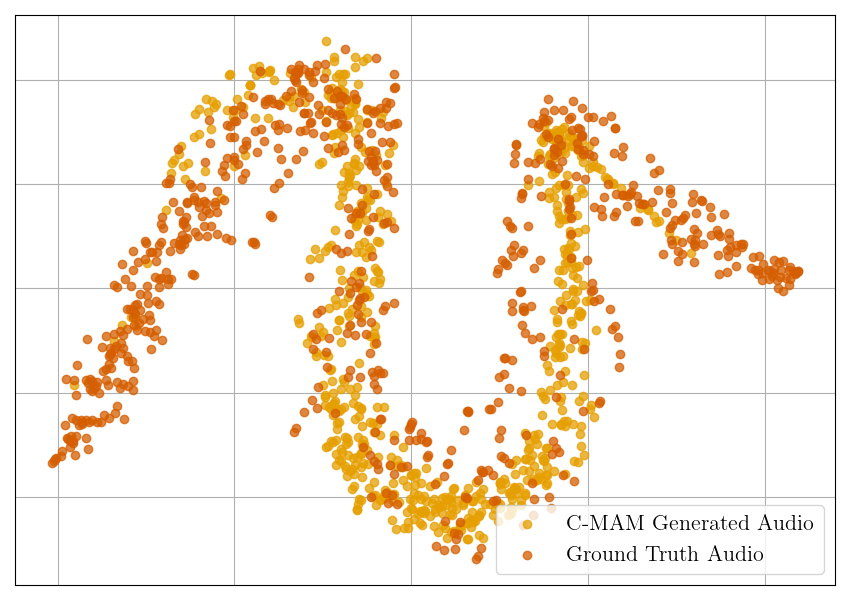
\includegraphics[width=\textwidth]{imgs/tsne/sns_audio_cmam_2.png}
        \caption*{AudioSet (V $\rightarrow$ A)}
    \end{subfigure}
    \begin{subfigure}[b]{0.24\textwidth}
        \centering
        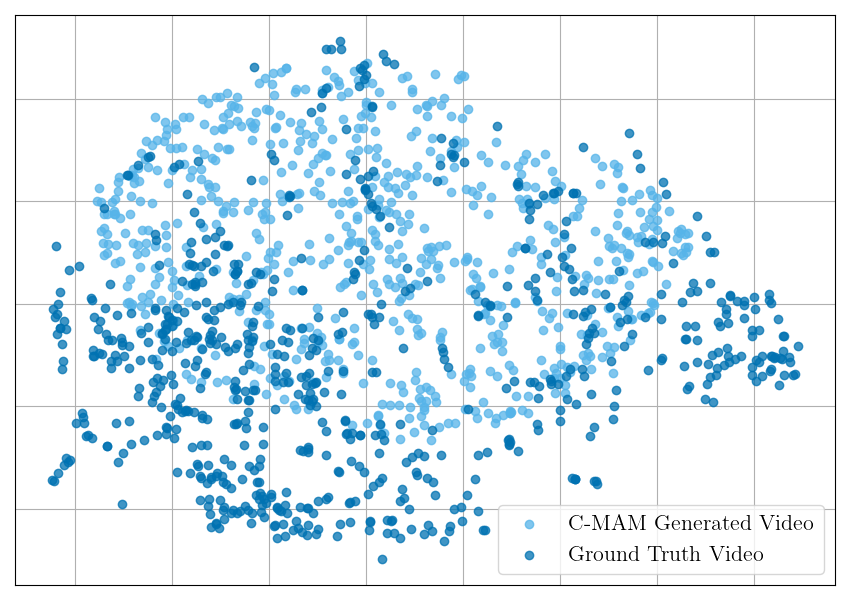
\includegraphics[width=\textwidth]{imgs/tsne/sns_video_cmam_3.png}
        \caption*{AudioSet (A $\rightarrow$ V)}
    \end{subfigure}
    \begin{subfigure}[b]{0.24\textwidth}
        \centering
        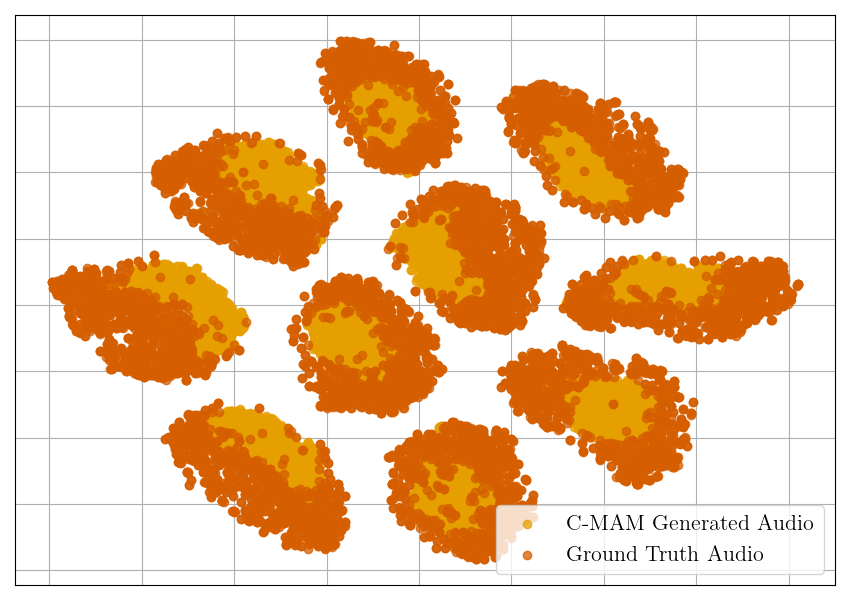
\includegraphics[width=\textwidth]{imgs/tsne/avmnist_audio_cmam_1.png}
        \caption*{AVMNIST (I $\rightarrow$ A)}
    \end{subfigure}
    \begin{subfigure}[b]{0.24\textwidth}
        \centering
        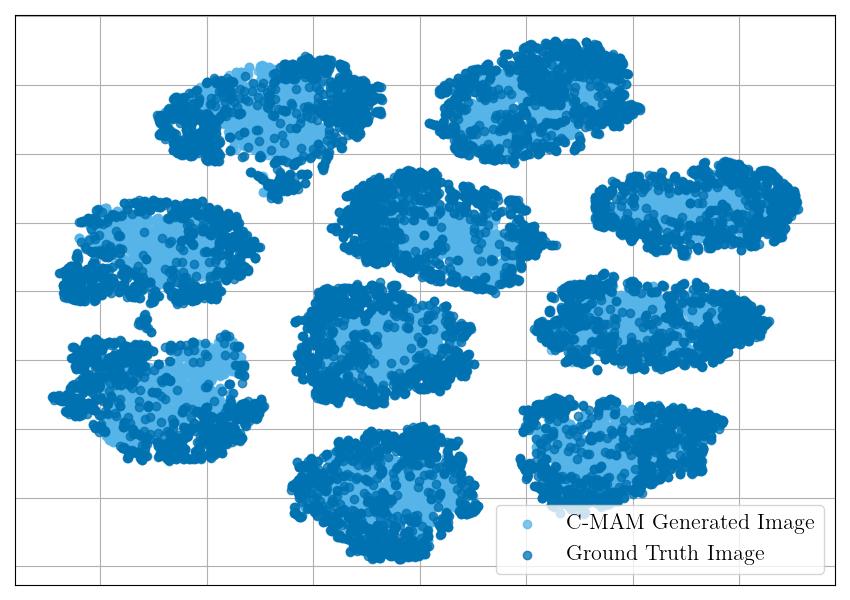
\includegraphics[width=\textwidth]{imgs/tsne/avmnist_video_cmam_1.png}
        \caption*{AVMNIST (A $\rightarrow$ I)}
    \end{subfigure}
    \centering
    \begin{subfigure}[b]{0.24\textwidth}
        \centering
        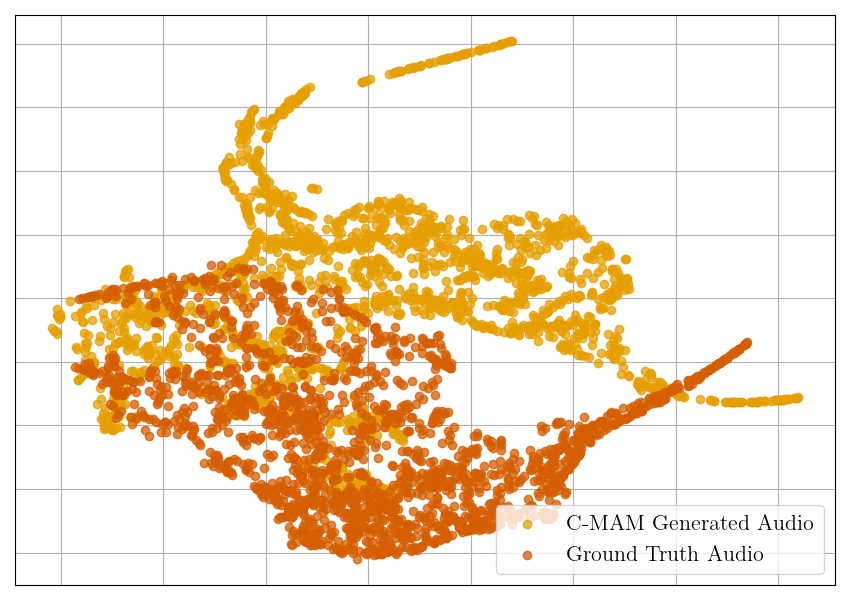
\includegraphics[width=\textwidth]{imgs/tsne/ks_audio_cmam_1.png}
        \caption*{Kinetics-Sounds (V $\rightarrow$ A)}
    \end{subfigure}
    \begin{subfigure}[b]{0.24\textwidth}
        \centering
        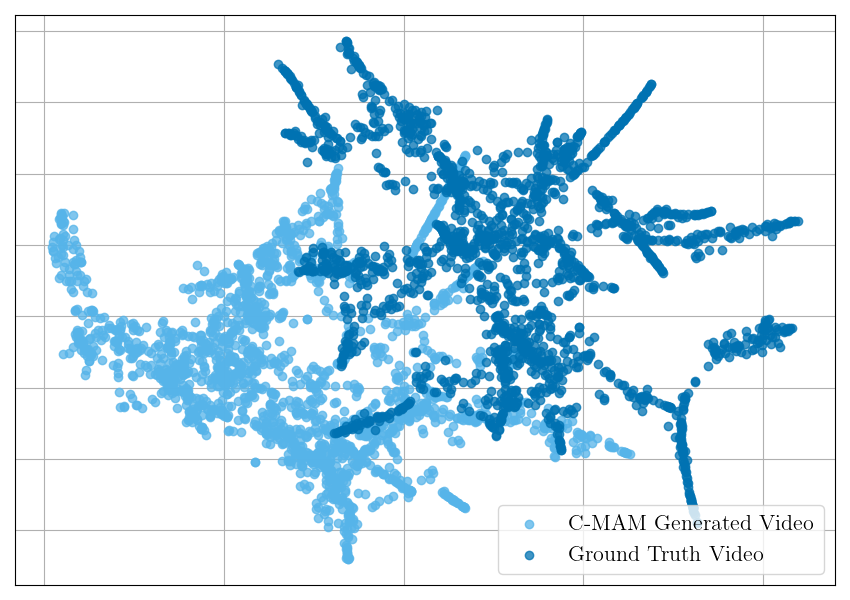
\includegraphics[width=\textwidth]{imgs/tsne/ks_video_cmam_1.png}
        \caption*{Kinetics-Sounds (A $\rightarrow$ V)}
    \end{subfigure}
    \begin{subfigure}[b]{0.24\textwidth}
        \centering
        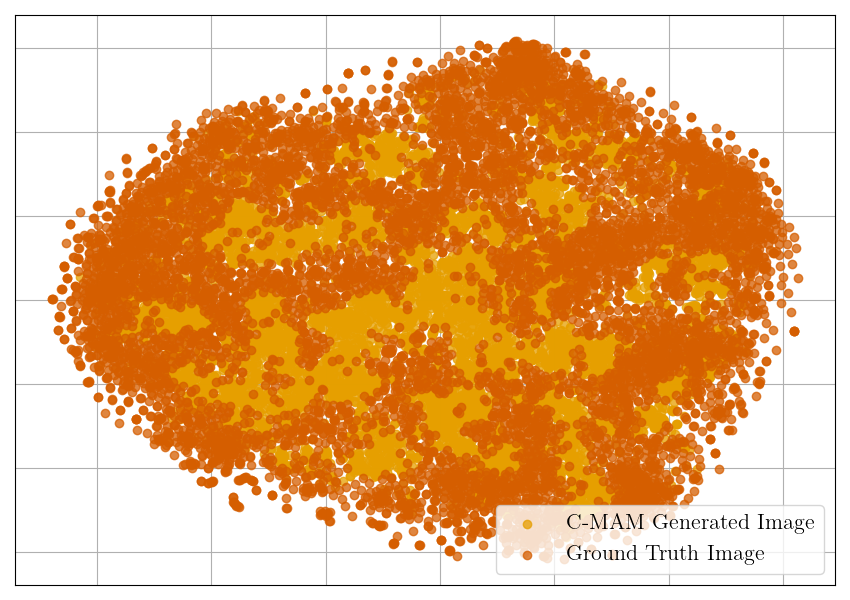
\includegraphics[width=\textwidth]{imgs/tsne/mmimdb_image_cmam_1.png}
        \caption*{MM-IMDb (T $\rightarrow$ I)}
    \end{subfigure}
    \begin{subfigure}[b]{0.24\textwidth}
        \centering
        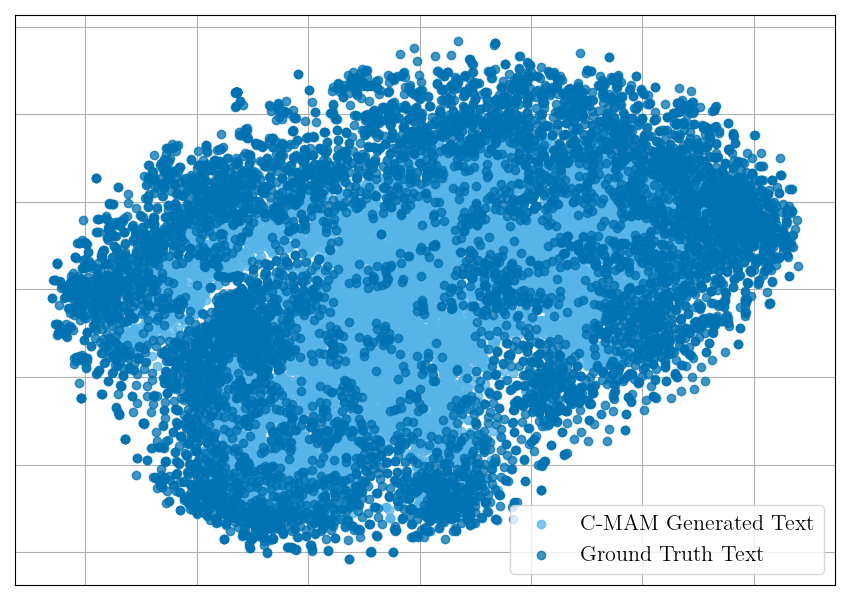
\includegraphics[width=\textwidth]{imgs/tsne/mmimdb_text_cmam_1.png}
        \caption*{MM-IMDb (I $\rightarrow$ T)}
    \end{subfigure}

    \centering

    \begin{subfigure}[b]{0.24\textwidth}
        \centering
        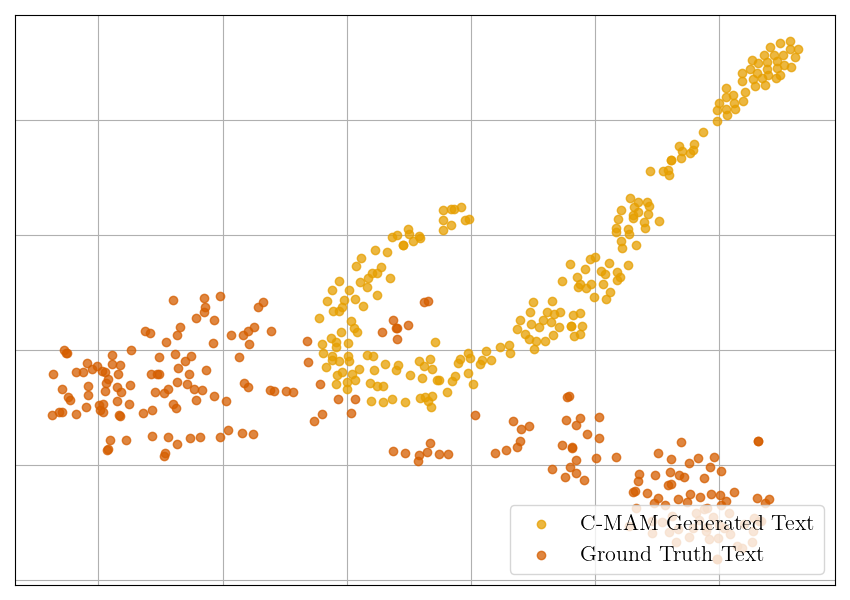
\includegraphics[width=\textwidth]{imgs/tsne/emt_dlfr_baseline_mosi_tsne.png}
        \caption*{EMT-DLFR MOSI (AV $\rightarrow$ T)}
    \end{subfigure}
    \begin{subfigure}[b]{0.24\textwidth}
        \centering
        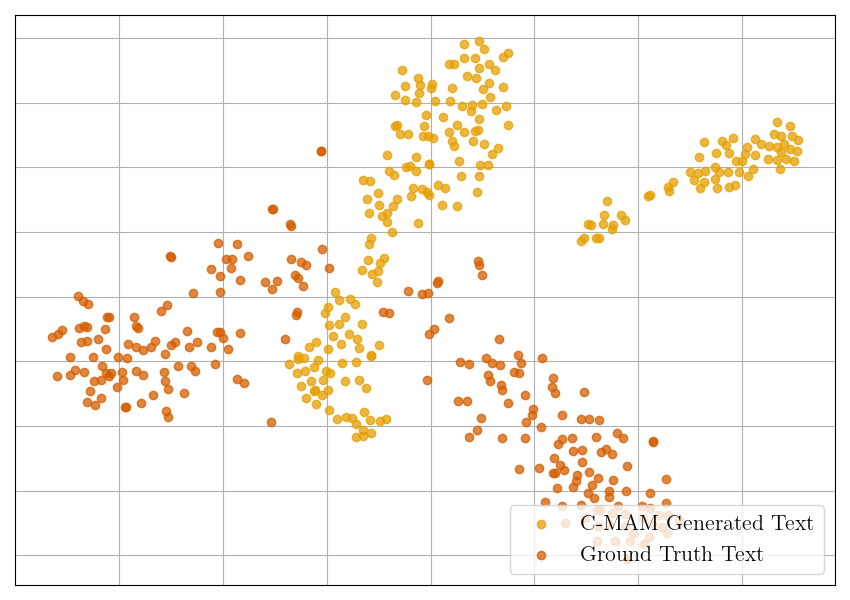
\includegraphics[width=\textwidth]{imgs/tsne/emt_dlfr_robust_baseline_mosi_tsne.png}
        \caption*{R. EMT-DLFR MOSI (AV $\rightarrow$ T)}
    \end{subfigure}
    \begin{subfigure}[b]{0.24\textwidth}
        \centering
        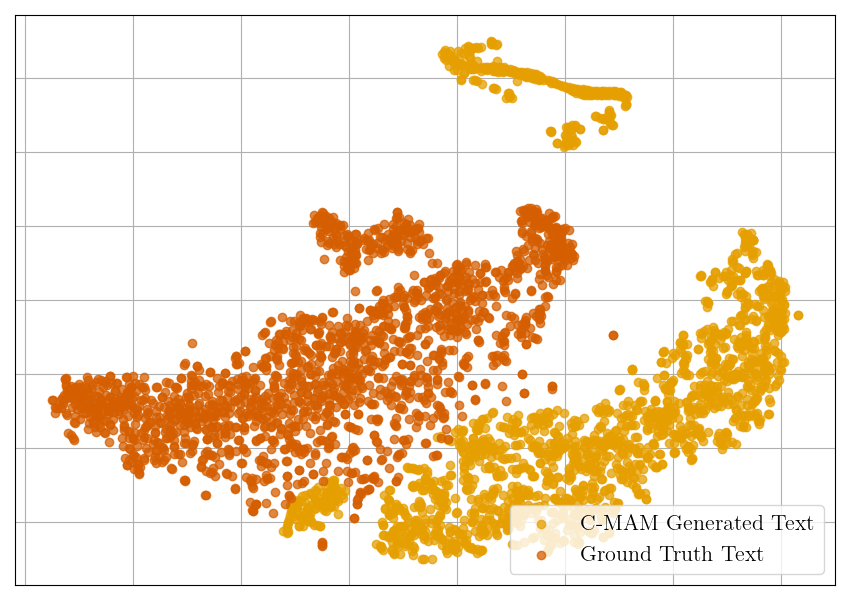
\includegraphics[width=\textwidth]{imgs/tsne/emt_dlfr_baseline_mosei_tsne.png}
        \caption*{EMT-DLFR MOSEI (AV $\rightarrow$ T)}
    \end{subfigure}
    \begin{subfigure}[b]{0.24\textwidth}
        \centering
        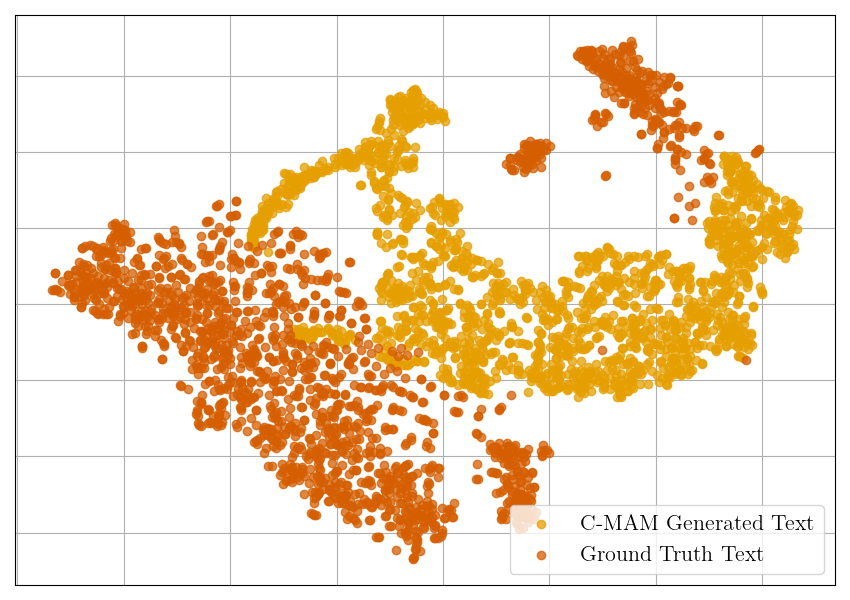
\includegraphics[width=\textwidth]{imgs/tsne/emt_dlfr_robust_baseline_mosei_tsne.png}
        \caption*{R. EMT-DLFR MOSEI (AV $\rightarrow$ T)}
    \end{subfigure}
\\
    \centering
    \begin{subfigure}[b]{0.24\textwidth}
        \centering
        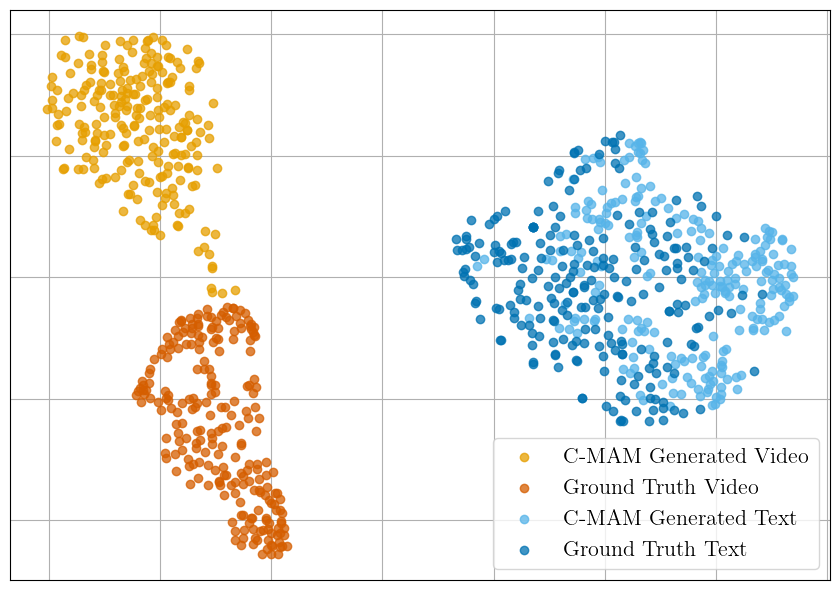
\includegraphics[width=\textwidth]{imgs/tsne/mmin/msp_improv/cmam_audio_tsne.png}
        \caption*{MSP-IMPROV (A $\rightarrow$ V+T)}
    \end{subfigure}
    \begin{subfigure}[b]{0.24\textwidth}
        \centering
        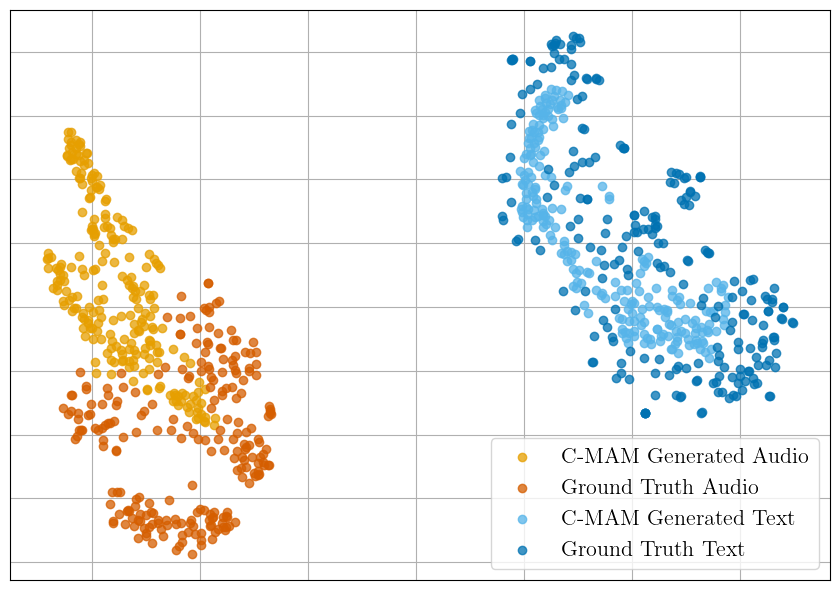
\includegraphics[width=\textwidth]{imgs/tsne/mmin/msp_improv/cmam_video_tsne.png}
        \caption*{MSP-IMPROV (V $\rightarrow$ A+T)}
    \end{subfigure}
    \begin{subfigure}[b]{0.24\textwidth}
        \centering
        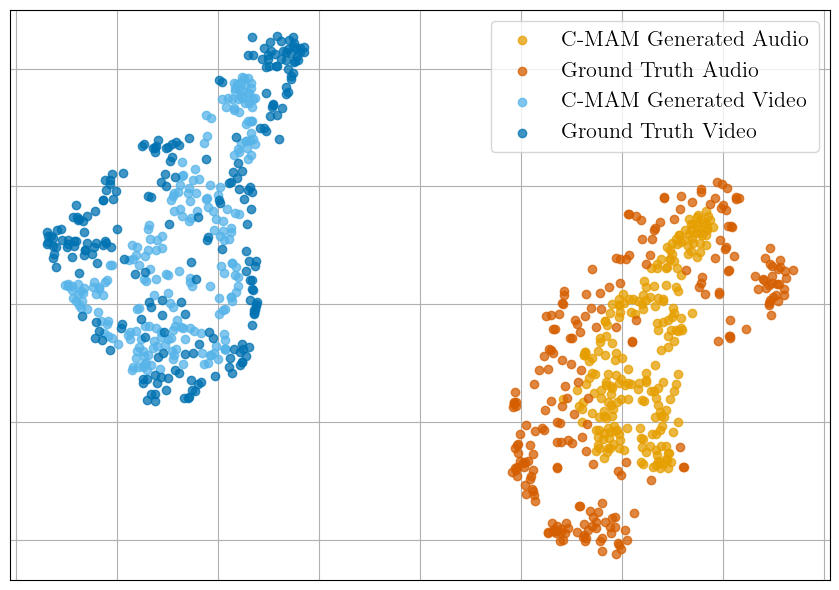
\includegraphics[width=\textwidth]{imgs/tsne/mmin/msp_improv/cmam_text_tsne.png}
        \caption*{MSP-IMPROV (T $\rightarrow$ A+L)}
    \end{subfigure}
    \begin{subfigure}[b]{0.24\textwidth}
        \centering
        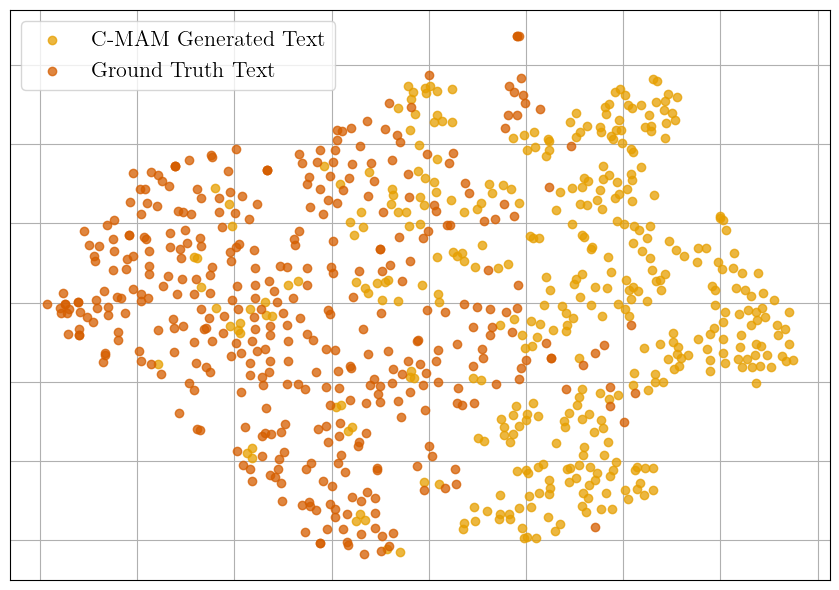
\includegraphics[width=\textwidth]{imgs/tsne/mmin/msp_improv/cmam_text_tsne_av.png}
        \caption*{MSP-IMPROV (AV $\rightarrow$ T)}
    \end{subfigure}
    \\
    \centering

    \begin{subfigure}[b]{0.24\textwidth}
        \centering
        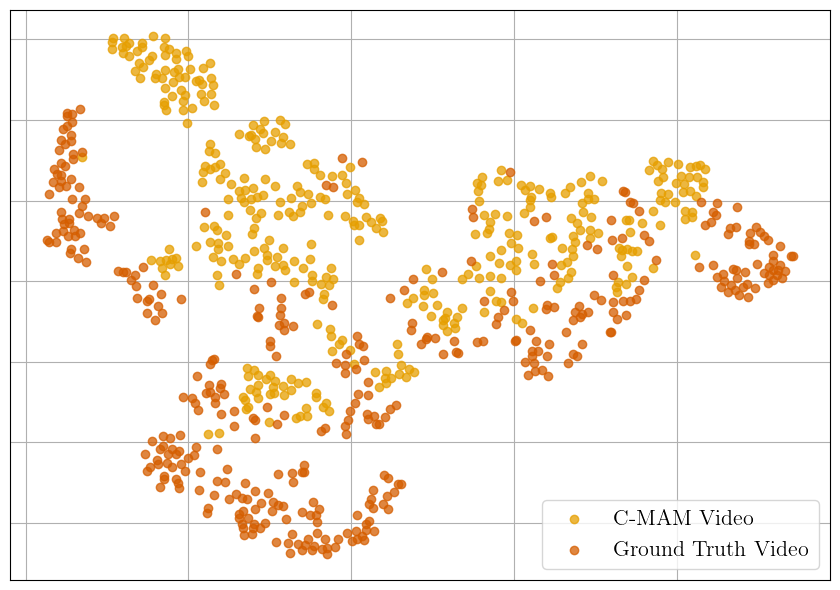
\includegraphics[width=\textwidth]{imgs/tsne/mmin/msp_improv/cmam_video_tsne_at.png}
        \caption*{MSP-IMPROV (AT $\rightarrow$ V)}
    \end{subfigure}
    \begin{subfigure}[b]{0.24\textwidth}
        \centering
        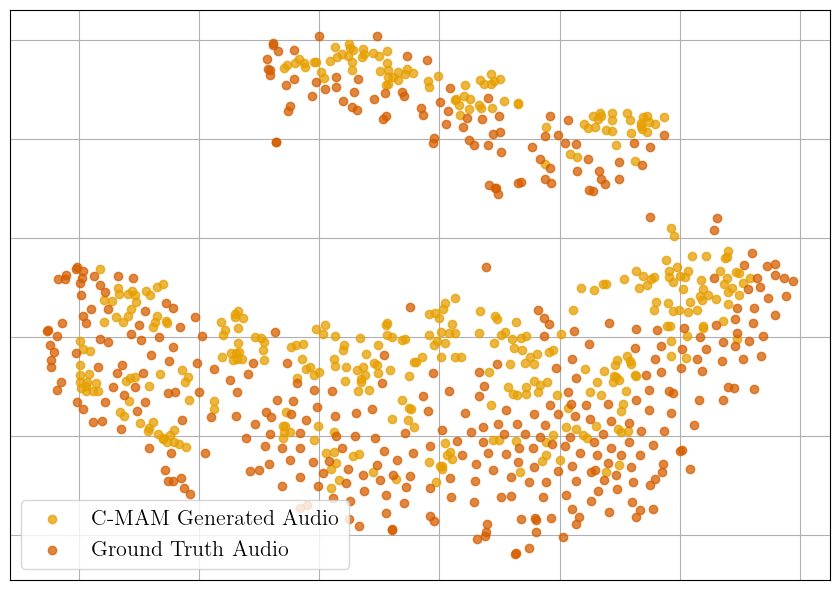
\includegraphics[width=\textwidth]{imgs/tsne/mmin/msp_improv/cmam_audio_tsne_vt.png}
        \caption*{MSP-IMPROV (VL $\rightarrow$ A)}
    \end{subfigure}
    \begin{subfigure}[b]{0.24\textwidth}
        \centering
        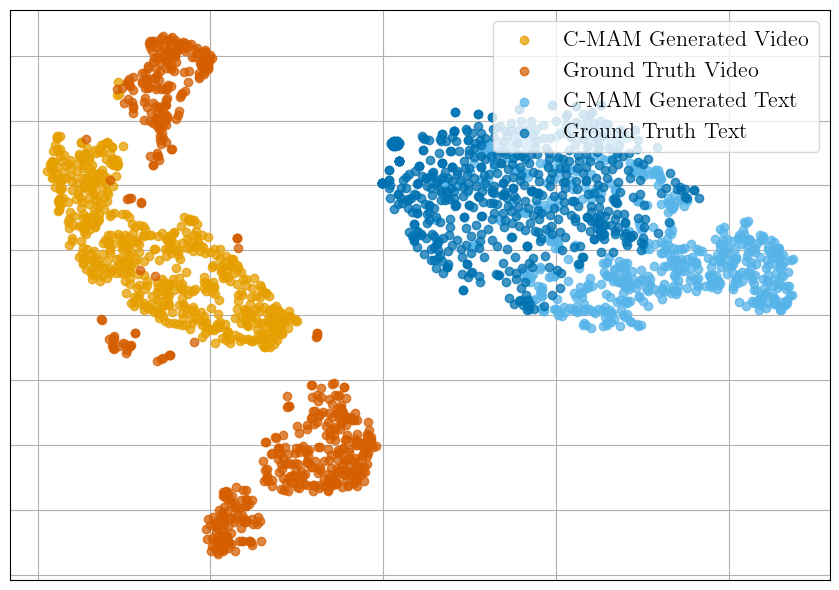
\includegraphics[width=\textwidth]{imgs/tsne/mmin/iemocap/cmam_audio_tsne.png}
        \caption*{IEMOCAP (A $\rightarrow$ V+T)}
    \end{subfigure}
    \begin{subfigure}[b]{0.24\textwidth}
        \centering
        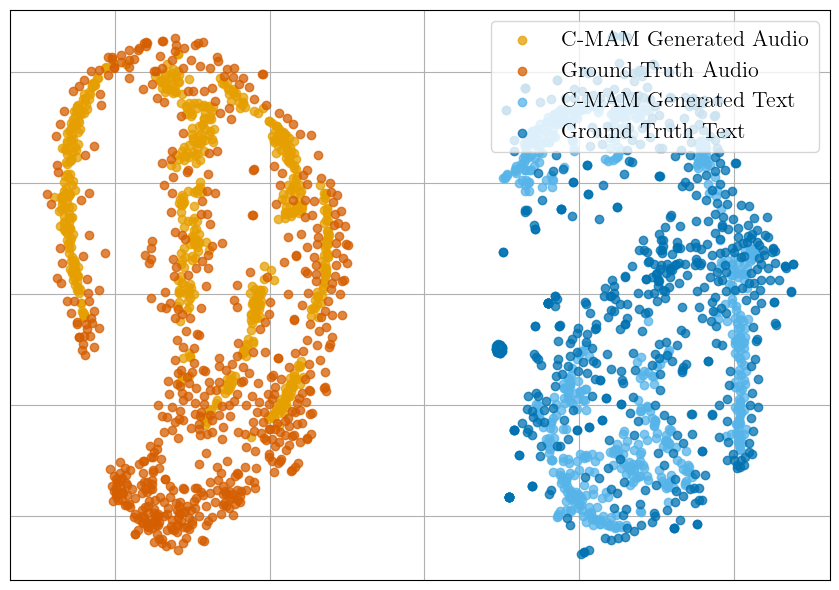
\includegraphics[width=\textwidth]{imgs/tsne/mmin/iemocap/cmam_video_tsne.png}
        \caption*{IEMOCAP (V $\rightarrow$ A+T)}
    \end{subfigure}
    \\
    \begin{subfigure}[b]{0.24\textwidth}
        \centering
        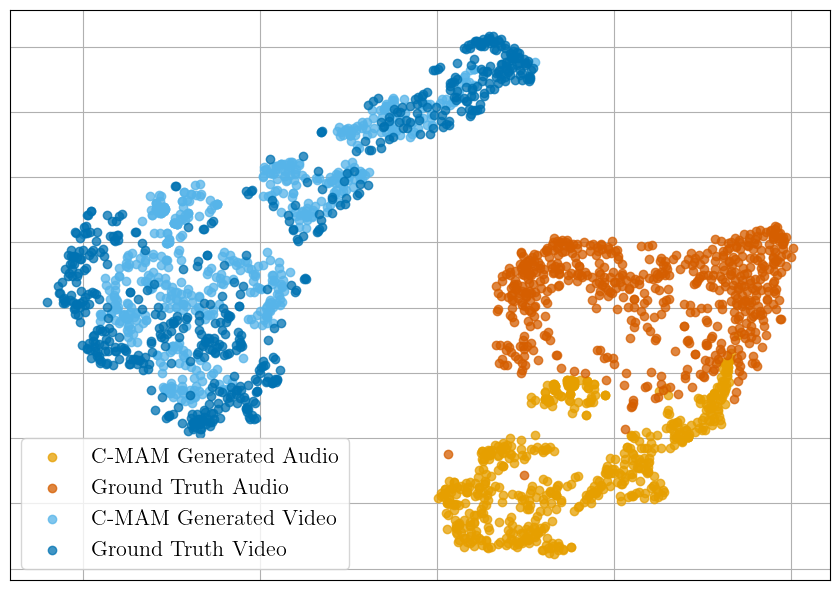
\includegraphics[width=\textwidth]{imgs/tsne/mmin/iemocap/cmam_text_tsne.png}
        \caption*{IEMOCAP (T $\rightarrow$ A+L)}
    \end{subfigure}
    \begin{subfigure}[b]{0.24\textwidth}
        \centering
        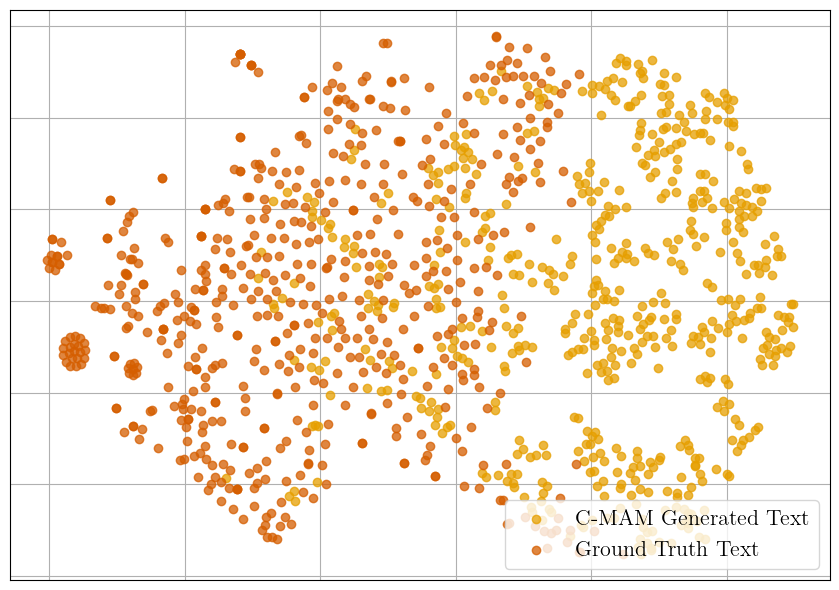
\includegraphics[width=\textwidth]{imgs/tsne/mmin/iemocap/cmam_gen_text_with_av.png}
        \caption*{IEMOCAP (AV $\rightarrow$ T)}
    \end{subfigure}
    \begin{subfigure}[b]{0.24\textwidth}
        \centering
        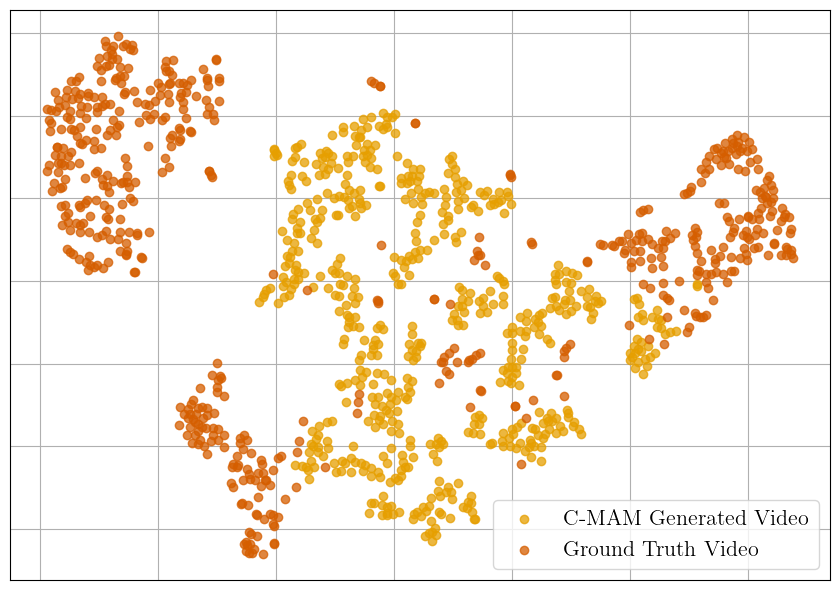
\includegraphics[width=\textwidth]{imgs/tsne/mmin/iemocap/cmam_gen_video_with_at.png}
        \caption*{IEMOCAP (AT $\rightarrow$ V)}
    \end{subfigure}
    \begin{subfigure}[b]{0.24\textwidth}
        \centering
        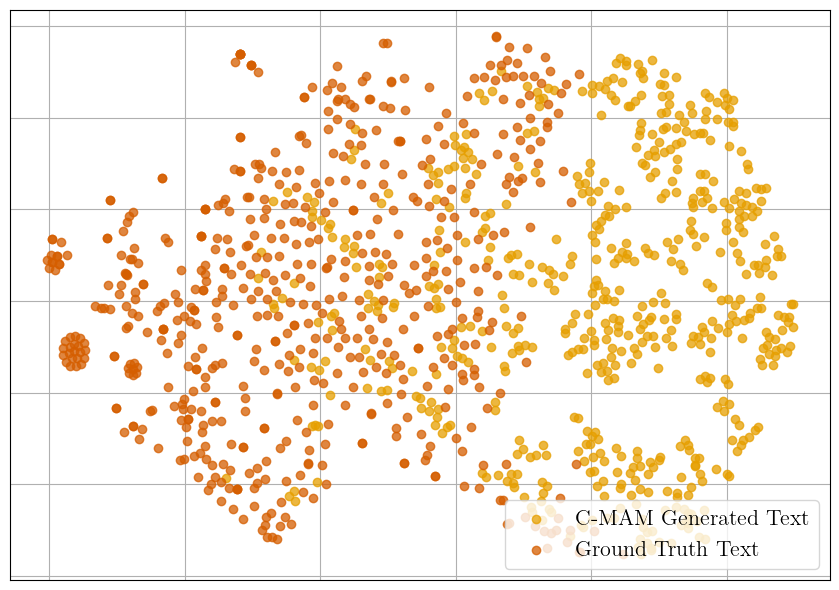
\includegraphics[width=\textwidth]{imgs/tsne/mmin/iemocap/cmam_gen_text_with_av.png}
        \caption*{IEMOCAP (VL $\rightarrow$ A)}
    \end{subfigure}
    \caption{T-SNE visualisations of the reconstructed embeddings vs. the ground truth features for each C-MAM trained.}
    \label{fig:tsne}

\end{figure}

% \end{landscape}

\textbf{C-MAM Reconstruction Error Metrics:} Table~\ref{tab:errors} presents reconstruction errors in terms of MAE and MSE for all the models tested in Section~\ref{sec:results}. Importantly, high reconstruction errors did not always correspond to poor performance recovery. This was particularly evident in the Kinetics-Sounds dataset, where despite significant reconstruction errors in the audio-to-video setting, C-MAMs still improved performance by 20\%-25\%. This suggests that the base multimodal model does not fully exploit all available modality information. C-MAMs can recover essential features even when the reconstructed embeddings are not exact replications of the ground truth. It also indicates how robust a multimodal model is to variances in the input data, as significant performance improvements were observed even when the reconstruction errors were high. The low error metrics demonstrate that C-MAMs effectively reconstruct missing modality embeddings.

\begin{table}[t!]
    \centering
    \caption{Error metrics between the ground truth feature embeddings produced by the trained modality-specific encoders and the C-MAM generated embeddings. Each row is organised as model - input modalities - output modality.}
    \label{tab:errors}
    \resizebox{\textwidth}{!}{%
    \begin{tabular}{l|cc|cc|l|cc}
    \hline
    \multirow{2}{*}{\textbf{Model \& C-MAM}}      & \multicolumn{2}{c|}{\textbf{IEMOCAP}} & \multicolumn{2}{c|}{\textbf{MSP-IMPROV}} & \multirow{2}{*}{\textbf{Model \& C-MAM}} & \multirow{2}{*}{\textbf{MAE}} & \multirow{2}{*}{\textbf{MSE}} \\ \cline{2-5}
                                                  & \textbf{MSE}      & \textbf{MSE}      & \textbf{MAE}        & \textbf{MSE}       &                                          &                               &                               \\ \hline
    \textbf{MMIN - Audio - Video}                 & 0.2205            & 0.1073            & 0.2106              & 0.0740             & \textbf{Audioset - Audio - Video}        & 0.3297                        & 0.1849                        \\
    \textbf{MMIN - Audio - Text}                  & 0.2272            & 0.1915            & 0.2691              & 0.3321             & \textbf{AudioSet - Video - Audio}        & 0.3804                        & 0.2190                        \\ \cline{6-8} 
    \textbf{MMIN - Audio/Video - Text}            & 0.2553            & 0.2387            & 0.2727              & 0.4158             & \textbf{AVMNIST - Audio - Image}         & 1.1611                        & 2.7552                        \\
    \textbf{MMIN - Audio/Text - Video}            & 0.0673            & 0.0089            & 0.0899              & 0.1413             & \textbf{AVMNIST - Image - Audio}         & 0.6106                        & 0.6121                        \\ \cline{6-8} 
    \textbf{MMIN - Video - Audio}                 & 0.0399            & 0.1558            & 0.2601              & 0.1158             & \textbf{Kinetics-Sounds - Audio - Video} & 3.8226                        & 32.7867                       \\
    \textbf{MMIN - Video - Text}                  & 0.2127            & 0.1955            & 0.1272              & 0.1825             & \textbf{Kinetics-Sounds - Video - Audio} & 0.6905                        & 1.3158                        \\ \cline{6-8} 
    \textbf{MMIN - Video/Text - Audio}            & 0.1044            & 0.0179            & 0.1282              & 0.0271             & \textbf{MM-IMDb - Image - Text}          & 0.2962                        & 0.1627                        \\
    \textbf{MMIN - Text - Audio}                  & 0.1917            & 0.0658            & 0.1547              & 0.0382             & \textbf{MM-IMDb - Text - Image}          & 0.2901                        & 0.1417                        \\
    \textbf{MMIN - Text - Video}                  & 0.0534            & 0.0071            & 0.0806              & 0.0133             &                                          &                               &                               \\ \cline{1-5}
    \textbf{}                                     & \multicolumn{2}{c|}{\textbf{MOSI}}    & \multicolumn{2}{c|}{\textbf{MOSEI}}      &                                          &                               &                               \\ \cline{1-5}
    \textbf{EMT-DLFR - Audio/Video - Text}        & 0.3461            & 0.2014            & 0.2690              & 0.1347             &                                          &                               &                               \\
    \textbf{Robust EMT-DLFR - Audio/Video - Text} & 0.3162            & 0.1886            & 0.3092              & 0.1657             &                                          & \multicolumn{1}{l}{}          & \multicolumn{1}{l}{}          \\ \hline
    \end{tabular}%
    }
\end{table}

\textbf{Statistical Analysis:} A detailed statistical analysis was conducted to quantify the alignment between reconstructed and ground-truth embeddings for the MM-IMDb, and MOSEI datasets. This analysis employed three complementary approaches: cosine similarity distributions to assess directional alignment, dimension-wise effect sizes to measure the magnitude of differences, and statistical significance tests to evaluate the reliability of these differences. Each dataset revealed distinct patterns in how C-MAMs preserve structural relationships in the latent space.

\begin{figure}[b!]
    \centering
    \includegraphics[width=0.875\textwidth]{imgs/MMIMDB/image_to_text/statstical_analysis.pdf}
    \includegraphics[width=0.875\textwidth]{imgs/MMIMDB/text_to_image/statstical_analysis.pdf}
    \caption{Statistical analysis of C-MAMs' reconstruction quality for the MM-IMDb dataset. The analysis includes a cosine similarity distribution, dimension-wise effect size analysis, and a volcano plot for mean difference significance.}
    \label{fig:mmimdb_stats}
\end{figure}

The \textbf{MM-IMDb} dataset and model presented a more nuanced picture of reconstruction effectiveness (see \Cref{fig:mmimdb_stats}). Despite showing relatively low directional alignment, with the Text-to-Image case exhibiting a mean cosine similarity of 0.051, C-MAMs enabled near-baseline performance recovery. This apparent contradiction prompted a dedicated sub-ablation study investigating whether explicitly optimising for directional alignment via cosine similarity loss would improve performance. The results, presented in Table~\ref{tab:mmimdb_sub_ablation}, revealed that neither pure cosine similarity loss nor a combined MSE and cosine similarity loss significantly improved reconstruction quality or performance metrics. This finding suggests that the multimodal model exhibits robustness to deviations in latent space alignment, with perfect cosine similarity not being a prerequisite for effective downstream classification.

\begin{table}[tb]
    \centering
    \caption{analysis of how varying the cosine loss term influences model performance metrics and embedding reconstruction in the MM-IMDb multimodal dataset.}
    \label{tab:mmimdb_sub_ablation}
    \resizebox{\textwidth}{!}{%
    \begin{tabular}{l|ccccc|ccccc}
    \hline
                            & \multicolumn{5}{c|}{\textbf{Image $\mapsto$ Text}}                                                      & \multicolumn{5}{c}{\textbf{Text $\mapsto$ Image}}                                                       \\ \cline{2-11} 
                            & \textbf{F1-Weighted} & \textbf{F1-Samples} & \textbf{F1-Micro} & \textbf{F1-Macro} & \textbf{Cos. Sim.} & \textbf{F1-Weighted} & \textbf{F1-Samples} & \textbf{F1-Micro} & \textbf{F1-Macro} & \textbf{Cos. Sim.} \\ \hline
    \textbf{MSE}            & 0.4019               & 0.4489              & 0.4577            & 0.2282            & 0.0974             & 0.5743               & 0.5986              & 0.6015            & 0.4232            & 0.0512             \\
    \textbf{Cos. Sim.}      & 0.4266               & 0.4302              & 0.4362            & 0.2695            & 0.1704             & 0.5148               & 0.5076              & 0.5128            & 0.3871            & 0.1430             \\
    \textbf{MSE + Cos. Sim} & 0.43088              & 0.4570              & 0.4658            & 0.2608            & 0.1556             & 0.5715               & 0.5877              & 0.5904            & 0.236             & 0.1253             \\ \hline
    \end{tabular}%
    }
\end{table}

\begin{figure}[pb!]
    \centering
    \includegraphics[width=0.875\textwidth]{imgs/MOSEI/audio_to_text/statstical_analysis.pdf}
    \includegraphics[width=0.875\textwidth]{imgs/MOSEI/audio_text_to_video/statstical_analysis.pdf}
    \caption{Statistical analysis of C-MAMs' reconstruction quality across a selection of missing conditions for the MOSEI dataset. Each includes a cosine similarity distribution, dimension-wise effect size analysis, and a volcano plot for mean difference significance. The remaining missing modality conditions are presented in the appendices.}
    \label{fig:mosei_stats}
\end{figure}

The \textbf{MOSEI} dataset analysis\footnote{See Section~\ref{sec:MOSEI} of the appendices for the analysis on all missing modality conditions trained the Utterance Fusion model \cite{zhao-etal-2021-missing} using the MOSEI dataset.} (see Figure~\ref{fig:mosei_stats}) revealed varying patterns across different modality combinations, providing insights into the relationship between reconstruction quality and model performance. The Audio-to-Text condition demonstrated strong directional alignment with right-skewed cosine similarity distributions. However, the volcano plot analysis revealed that many dimensions still exhibited statistically significant differences, despite effect sizes being near zero. The Audio and Text-to-Video condition showed moderately strong alignment with a mean cosine similarity of 0.78 and median of 0.80. However, effect size analysis indicated the presence of small but statistically significant deviations. These patterns suggest that while C-MAMs achieve strong overall latent space alignment, the presence of small dimensional deviations does not impact downstream performance significantly.

The collective findings from this statistical analysis reveal three key insights about C-MAM behaviour. First, the degree of embedding alignment achieved by C-MAMs varies across datasets and modality combinations, suggesting that different modality pairs may require different levels of reconstruction precision. Second, strong performance improvements can be achieved even with imperfect reconstruction, indicating that multimodal models are robust to certain embedding deviations. Third, statistically significant dimensional differences do not necessarily correspond to degraded performance, suggesting that some embedding dimensions may be redundant or non-critical for the downstream task. These insights validate the effectiveness of C-MAMs and guide future optimisation of missing modality reconstruction techniques.

\textbf{Contrastive Information in Learned Embeddings: } Multimodal learning is often assumed to benefit from mutual and complementary information across modalities. However, our analysis reveals that modality-specific encoders do not always preserve these relationships, as \textit{contrastive embeddings} can emerge during training. In such cases, embeddings from different modalities become misaligned in feature space, which can reduce their informativeness when combined. The impact on downstream performance depends on the extent of contrastiveness, the nature of the task, and whether the fusion and classification layers compensate for misaligned features.

To better understand this, we analysed learned modality embeddings across AVMNIST, Kinetics-Sounds, and MOSEI. Kinetics-Sounds exhibited the strongest contrastive behaviour, with high KL divergence and near-zero cosine similarity between audio and video embeddings, indicating that the model disregarded audio features entirely. MOSEI showed moderate contrastiveness, where the dominance of text led to weaker reliance on audio and video. In AVMNIST, contrastive embeddings were present, yet performance remained unaffected. This demonstrates that contrastiveness does not always degrade results. Even misaligned embeddings can still support accurate reconstruction when a task is highly redundant, as in digit classification.

Contrastive embeddings are not necessarily an inherent dataset property but can emerge due to the training dynamics of modality-specific encoders. While contrastiveness can impact missing modality reconstruction, its effect depends on whether the fusion mechanism and classifier can compensate for the misalignment. In AVMNIST, the classifier extracted class-relevant features despite embeddings being nearly orthogonal, allowing C-MAMs to achieve full performance recovery. In contrast, Kinetics-Sounds showed that when contrastiveness is severe and fusion cannot realign features, one modality may be ignored, leading to degraded performance when it is missing.

Despite evidence of contrastive embeddings across all datasets, \textbf{C-MAMs remained highly effective in recovering missing modality performance}. Their ability to restore meaningful information, even in contrastive settings, suggests that contrastive embeddings do not always prevent reconstruction but may introduce additional challenges depending on how well learned features align. Further details and statistical analyses are provided in Appendix~\ref{sec:contrastive_info}.

\textbf{C-MAM Data Requirements:} A key consideration in the post-training C-MAM approach is the requirement to train new C-MAMs on the full dataset, which can be computationally expensive. We conduct experiments using progressively larger balanced subsets (10\%-100\%) of AVMNIST, MM-IMDb, and MOSEI to assess the minimum training data necessary, evaluating C-MAMs on the full test set. The results show that \textbf{C-MAMs trained with as little as 10\% of the data achieve strong performance}, with only minor differences from full dataset training. Larger datasets lead to faster convergence but not necessarily better final performance, suggesting that \textit{learnt latent spaces remain robust} even with limited training. In MM-IMDb, stronger modality dependence causes greater instability at lower data availability, though test performance remains stable. In MOSEI, text-based conditions are largely unaffected by training size, reinforcing the \textit{importance of modality-specific learning dynamics}.

These findings highlight the \textit{efficiency of learning a static latent space post-training}, which remains transferable across different training conditions. Full experimental results are provided in the appendix.

\textbf{Observability into Multimodal Model Performance:} This work emphasises detailed evaluation of missing modality conditions, an often-overlooked aspect of multimodal learning. Many studies assess robustness in aggregate, neglecting how missing modalities impact latent space structure and performance. Our experiments show that even with low cosine similarity between reconstructed and ground-truth embeddings, C-MAMs can still recover task performance. This is especially evident in MM-IMDb, where Text-to-Image reconstruction yielded low similarity yet restored F1 scores to the baselines. These findings highlight the need for task-aware evaluations over standard embedding similarity metrics. Beyond performance reporting, we provide embedding visualisations, statistical significance tests, and effect size analyses, revealing that statistically significant deviations in individual dimensions do not necessarily harm inference. Future work should explore whether these insights generalise across architectures and whether tools like SHAP or saliency maps could enhance interpretability. As multimodal models see real-world deployment, a standardised missing modality evaluation framework is crucial. Our results suggest comprehensive error analysis, visualisation techniques, and task-aware evaluations are essential for assessing robustness to missing data.


\textbf{Limitations and Future Directions:} While C-MAMs offer a modular solution for missing modality reconstruction, their effectiveness \textbf{depends on the base multimodal model's learned representations}. Reconstruction may have limited impact if a modality is underutilised during training, making C-MAMs ineffective in addressing inherent modality imbalances. \textbf{Scalability} remains a challenge, as the number of required C-MAMs grows exponentially (the total can be expressed as $2^K - 2$) with the number of modalities. Training separate models for each missing modality scenario increases computational overhead. Research into multimodal reconstruction strategies that generalise across missing conditions without sacrificing specificity could improve efficiency. However, given the strong performance of the current approach, additional complexity should be introduced only where meaningful gains are observed. C-MAMs also require \textbf{access to the original dataset} for training, which may pose challenges in privacy-sensitive applications and requires an investigation into training C-MAMs using privacy-preserving techniques and minimal amounts of data. Furthermore, while MSE has proven effective, it does not explicitly enforce semantic consistency. Future work could explore alternative loss functions, such as contrastive learning, to improve reconstruction alignment. 

Beyond these technical improvements, future work should also establish standardised evaluation frameworks for missing modality reconstruction, considering both reconstruction quality and downstream task performance. Addressing these limitations while preserving simplicity and flexibility will be key to ensuring broader applicability as multimodal systems expand.



\section{Conclusion}\label{sec:conc}
Missing modality data presents a fundamental challenge in deploying multimodal machine learning systems, particularly in real-world applications where sensor failures, resource constraints, or privacy restrictions can lead to incomplete modality information. This paper introduced \textit{Cross-Modal Association Models} (C-MAMs), demonstrating that a simple, modular approach to post-hoc missing modality reconstruction can effectively maintain multimodal model performance without requiring modifications to the base architecture or training process.

We validated three key contributions through comprehensive empirical evaluation across six multimodal models, eight datasets, and four distinct modalities. First, C-MAMs significantly improved inference-time performance, achieving up to 39\%, 30\%, and 28\% improvements in AVMNIST, MM-IMDb, and IEMOCAP respectively, compared to missing modality baselines. Second, detailed statistical analysis revealed that C-MAMs can effectively reconstruct missing modality embeddings even when perfect latent space alignment is not achieved, demonstrating the robustness of multimodal models to embedding deviations. Third, we showed that a straightforward architecture using MSE loss and minimal data can produce effective reconstructions, challenging the assumption that complex generative models or contrastive learning frameworks are necessary for handling missing modalities.

\textbf{Limitations and Future Work:} While C-MAMs provide an effective solution for missing modality reconstruction, several important limitations warrant further investigation. The exponential growth in required C-MAMs with increasing modality count presents scalability challenges in high-dimensional settings. Future work should explore techniques for reducing model redundancy while maintaining reconstruction effectiveness. Additionally, the dependence on base model representations means that C-MAMs cannot overcome inherent modality imbalances in the original training. Research into more sophisticated reconstruction architectures and loss functions could address these limitations while maintaining the core benefits of simplicity and modularity.

\textbf{Broader Implications:} The success of C-MAMs in post-hoc missing modality reconstruction has significant implications for real-world multimodal systems. Their modular design and deployment flexibility make them particularly suitable for distributed learning environments such as federated learning and Internet of Things applications, where different nodes may have access to varying subsets of modalities. In healthcare settings, for instance, C-MAMs could enable robust diagnosis across hospitals with varying sensor capabilities without requiring centralized data collection or model retraining. The demonstrated effectiveness of simple reconstruction approaches also suggests that complex architectural solutions may not always be necessary for practical multimodal problems, encouraging future research to evaluate the trade-offs between model complexity and performance gains carefully.

In conclusion, this work establishes C-MAMs as a practical and effective solution for handling missing modality data in multimodal learning. By enabling flexible, post-hoc reconstruction without compromising base model integrity, C-MAMs address a critical gap in existing approaches to missing modality handling. The comprehensive empirical evaluation and statistical analysis presented in this study validate the effectiveness of C-MAMs and provide valuable insights into the relationship between embedding reconstruction quality and downstream task performance. These findings lay the groundwork for more robust and adaptable multimodal systems while highlighting important directions for future research in this critical area of machine learning.

\section*{Acknowledgements}
This work was conducted with the financial support of the Science Foundation Ireland Centre for Research Training in Digitally-Enhanced Reality (d-real) under Grant No. 18/CRT/6224. For the purpose of Open Access, the author has applied a CC BY public copyright licence to any Author Accepted Manuscript version arising from this submission

\bibliographystyle{ACM-Reference-Format}
\bibliography{refs}
% \
\section{Appendix}
\label{sec:appendix}
The following sections provide supplementary material for the main paper. \Cref{sec:reproducibility,sec:hyperparameters} discusses the reproducibility of the experiments conducted in the main paper and provides the hyperparameters used. \Cref{sec:reproducibility_exp3} includes further information on the models and C-MAMs trained in experiment three. \Cref{sec:contrib} presents and discusses experimental results investigating the contribution of each modality to C-MAM performance for the models tested in experiment 3. \Cref{sec:MOSEI} then provides the results of evaluating C-MAMs on the MOSEI dataset using the Utterance Fusion baseline model. Alongside the performance metrics, we also present the reconstruction errors, T-SNE Visualisations and the complete statistical analysis of the C-MAMs' reconstruction quality across the missing conditions. \Cref{sec:additional_results} provides additional performance results of the models evaluated in the experiments. Finally, \Cref{sec:hyperparameters} provides the hyperparameters used for the models trained on the AudioSet, AV-MNIST, Kinetics-Sounds, and MMIMDB datasets.

\subsection{Reproducibility}\label{sec:reproducibility}
The code used for implementing and evaluating C-MAMs will be made publicly available on GitHub upon publication, with a link in this paper's final version. 
Experiments were conducted on a desktop system with an Intel i7-13700K processor, 32GB RAM, and an Nvidia RTX 3070 GPU.
To ensure reproducibility, the main text and appendix describe all relevant experimental details, including dataset preprocessing, hyperparameter choices, and evaluation procedures. The provided code will include all necessary components to replicate the reported results.

\subsection{Experiment 3: C-MAMs}
\label{sec:reproducibility_exp3}
We used the official repositories and the hyperparameters provided for all baseline models trained in experiment three. For both models, we recreated the results to within approximately 2\%, which can be attributed to the random seeds used. 

The C-MAMs used for experiment three comprise the modality-specific encoders from the baseline models. The association networks were composed of three linear layers with batch normalisation, dropout and ReLU activations for the EMT-DLFR model, and for MMIN, three variations were used; two linear layers with batch normalisation, dropout and ReLU activations, ReLU and dropout for the output of the encoder, followed by two linear layers with batch normalisation, dropout and ReLU activations and finally the bimodal variation which includes two linear layers (the input layer is wider) with batch normalisation, dropout and ReLU activations. The C-MAMs were trained using Adam optimisation, a $1e^{-3}$ learning rate, batch size of $128$ and MSE loss. They were trained over 100 epochs during which the best-performing models were saved for evaluation.

\FloatBarrier

\subsection{Minimum Training Requirements}\label{sec:min_training}
A key consideration in the post-training C-MAM approach is the requirement to train new C-MAMs on the full dataset. Since each C-MAM is trained independently, this process can be computationally expensive. To assess the minimum training data necessary for effective performance, we conduct experiments using progressively larger balanced subsets (10\%–100\%) of AVMNIST, MM-IMDb, and MOSEI, evaluating C-MAMs on the full test set after training.

\textbf{AVMNIST:} The results in \Cref{fig:avmnist_min_training} indicate that C-MAMs trained with as little as 10\% of the data still achieve strong performance, with differences of approximately 5\% (Audio to Image) and 2\% (Image to Audio) when compared to full dataset training. The validation loss curves demonstrate a common trend across all data percentages, showing that while larger datasets lead to faster and more stable convergence, even small training subsets enable effective learning. This suggests that the \textbf{latent space learnt during training remains robust}, allowing smaller training samples to reconstruct missing modalities effectively. Notably, the Image to Audio C-MAM exhibits greater instability at lower data availability, likely due to \textbf{asymmetry in information redundancy between modalities}.

\begin{figure}[h!]
    \centering
    \includegraphics[width=0.475\linewidth]{imgs/min_training/avmnist_audio_to_image.pdf}
    \includegraphics[width=0.475\linewidth]{imgs/min_training/avmnist_image_to_audio.pdf}
    \includegraphics[width=0.475\linewidth]{imgs/min_training/avmnist_audio_to_image_val_loss.pdf}
    \includegraphics[width=0.475\linewidth]{imgs/min_training/avmnist_image_to_audio_val_loss.pdf}
    \caption{\textbf{AVMNIST: }\textbf{Top}: C-MAM classification performance versus percentage of training data available. \textbf{Bottom}: Validation loss during C-MAM training performance versus percentage of training data available.}
    \label{fig:avmnist_min_training}
\end{figure}

\textbf{MM-IMDb:} \Cref{fig:mmimdb_min_training} presents similar trends but highlights dataset-specific challenges. While performance differences remain small (4\%–10\% for Image to Text, 2\%–5\% for Text to Image), the loss curves reveal that \textbf{low training availability leads to increased instability}, particularly in early training epochs. The \textbf{modality dependence in MM-IMDb is more pronounced}, as text provides stronger supervision for genre classification. However, the Text to Image and Image to Text C-MAMs exhibit similar stability trends, with fluctuations primarily occurring at lower training data availability and reinforcing the idea that \textbf{latent space alignment is more challenging when the source modality carries weaker supervisory signals}. Despite this, test performance remains stable across all training subsets, suggesting that the \textbf{learnt latent spaces generalize well} to unseen data, even when trained with limited samples.

\begin{figure}[h!]
    \centering
    \includegraphics[width=0.475\linewidth]{imgs/min_training/mmimdb_image_to_text.pdf}
    \includegraphics[width=0.475\linewidth]{imgs/min_training/mmimdb_text_to_image.pdf}
    \includegraphics[width=0.475\linewidth]{imgs/min_training/mmimdb_image_to_text_val.pdf_loss.pdf}
    \includegraphics[width=0.475\linewidth]{imgs/min_training/mmimdb_text_to_image_val.pdf_loss.pdf}
    \caption{\textbf{MM-IMDb: } \textbf{Top:} C-MAM classification performance versus percentage of training data available. \textbf{Bottom:} Validation loss during C-MAM training performance versus percentage of training data available.}
    \label{fig:mmimdb_min_training}
\end{figure}

\textbf{MOSEI:} The results in \Cref{fig:mosei_min_training_two,fig:mosei_min_training_three,fig:mosei_min_training_four,fig:mosei_min_training_five,fig:mosei_min_training_six} further support these conclusions. The Audio to Text, Video to Text, and Audio and Video to Text C-MAMs exhibit clear performance gains with increasing training data, aligning with prior observations in \Cref{tab:mosei_results}. However, for cases where text is available, performance remains largely unaffected by training size, reinforcing the \textbf{dominance of text as a supervisory modality} in multimodal tasks. Across all conditions, validation loss curves follow similar patterns, with larger training subsets enabling faster convergence. The slower learning curves for smaller training sizes, despite ultimately reaching comparable performance, highlight the \textbf{efficiency of the learnt latent spaces in adapting to missing modalities with minimal data}.


Overall, these findings emphasize the \textbf{robustness of the learnt latent spaces in the C-MAM framework}. Even with limited training data, the representations enable effective reconstruction and generalization. The results further support the conclusion that \textbf{learning a learnt, static latent space post-training offers significant advantages over working directly with the original model and data}, as they remain transferable and stable across different training conditions. Additionally, the interplay between modality dominance and training efficiency suggests that future research could explore \textbf{adaptive training strategies}, selectively allocating training resources based on modality importance to optimise computational efficiency further.

\begin{figure}[h!]
    \centering
    \includegraphics[width=0.475\linewidth]{imgs/min_training/mosei_audio_to_video.pdf}
    \includegraphics[width=0.475\linewidth]{imgs/min_training/mosei_audio_to_text.pdf}
    \includegraphics[width=0.475\linewidth]{imgs/min_training/mosei_audio_to_video_loss.pdf}
    \includegraphics[width=0.475\linewidth]{imgs/min_training/mosei_audio_to_text_loss.pdf}


    \caption{\textbf{MOSEI:} \textbf{Top:} Audio C-MAM classification performance versus percentage of training data available. \textbf{Bottom: } Validation loss during C-MAM training performance versus percentage of training data available.}
    \label{fig:mosei_min_training_two}
\end{figure}


\begin{figure}[h!]
    \includegraphics[width=0.475\linewidth]{imgs/min_training/mosei_video_to_audio.pdf}
    \includegraphics[width=0.475\linewidth]{imgs/min_training/mosei_video_to_text.pdf}
    \includegraphics[width=0.475\linewidth]{imgs/min_training/mosei_video_to_audio_loss.pdf}
    \includegraphics[width=0.475\linewidth]{imgs/min_training/mosei_video_to_text_loss.pdf}
    \caption{\textbf{MOSEI:} \textbf{Top:} Video C-MAM classification performance versus percentage of training data available. \textbf{Bottom:} Validation loss during C-MAM training performance versus percentage of training data available.}
    \label{fig:mosei_min_training_three}
\end{figure}

\begin{figure}[h!]
    \includegraphics[width=0.475\linewidth]{imgs/min_training/mosei_text_to_audio.pdf}
    \includegraphics[width=0.475\linewidth]{imgs/min_training/mosei_text_to_video.pdf}
    \includegraphics[width=0.475\linewidth]{imgs/min_training/mosei_text_to_audio_loss.pdf}
    \includegraphics[width=0.475\linewidth]{imgs/min_training/mosei_text_to_video_loss.pdf}
    \caption{\textbf{MOSEI:} \textbf{Top:} Text C-MAM classification performance versus percentage of training data available. \textbf{Bottom:} Validation loss during C-MAM training performance versus percentage of training data available.}
    \label{fig:mosei_min_training_four}
\end{figure}

\begin{figure}[h!]

    \includegraphics[width=0.475\linewidth]{imgs/min_training/mosei_audio_video_to_text.pdf}
    \includegraphics[width=0.475\linewidth]{imgs/min_training/mosei_audio_text_to_video.pdf} 
    \includegraphics[width=0.475\linewidth]{imgs/min_training/mosei_audio_video_to_text_loss.pdf}
    \includegraphics[width=0.475\linewidth]{imgs/min_training/mosei_audio_text_to_video_loss.pdf} 
    \caption{\textbf{MOSEI:} \textbf{Top:} Audio-Video and Audio-Text C-MAM classification performance versus percentage of training data available. \textbf{Bottom:} Validation loss during C-MAM training performance versus percentage of training data available.}
    \label{fig:mosei_min_training_five}

\end{figure}


\begin{figure}[b!]
    \includegraphics[width=0.475\linewidth]{imgs/min_training/mosei_video_text_to_audio.pdf}
    \includegraphics[width=0.475\linewidth]{imgs/min_training/mosei_video_text_to_audio_loss.pdf}
    \caption{\textbf{MOSEI:} \textbf{Top:} Video-Audio and Video-Text C-MAM classification performance versus percentage of training data available. \textbf{Bottom:} Validation loss during C-MAM training performance versus pe                                              rcentage of training data available.}
    \label{fig:mosei_min_training_six}
\end{figure}


\FloatBarrier

\subsection{Bi-modal C-MAM Contributions}\label{sec:contrib}
Table~\ref{tab:contributions} evaluates C-MAMs in bimodal settings where a single modality is missing. The results confirm that the generated features consistently improved performance, though the extent of improvement depended on the base model's reliance on the missing modality. If a model inherently underutilises a particular modality, the C-MAM's ability to recover performance is limited by the degree to which the missing modality initially contributed to inference. The results also demonstrate that the C-MAMs, like any other multimodal model, are susceptible to using modality data in an imbalanced manner. For example, in MOSEI, removing the text modality caused a substantial drop in accuracy, indicating its dominant role in the model's decision-making. In contrast, missing audio or video led to minimal performance degradation, suggesting that the model already relied predominantly on textual information. This highlights a fundamental limitation: if a modality is not critical to the base model's predictions, its reconstruction via C-MAMs will not substantially improve performance.

\subsection{Analysis of Contrastive Information Across Datasets}\label{sec:contrastive_info}

Multimodal learning is typically assumed to leverage mutual and complementary information between modalities. However, this is not always the case in practice, as \textit{contrastive information}, where modality embeddings interfere with rather than enhance each other, can emerge due to training dynamics. To investigate this phenomenon, we analyze the \textit{learned modality-specific embeddings} in three datasets (AVMNIST, Kinetics-Sounds, and MOSEI) using a combination of statistical dependency tests. Our objective is to determine whether contrastive information exists in the model’s learned embeddings and how it affects missing modality reconstruction.

For each dataset, we compute \textit{mutual information} (MI), \textit{conditional entropy} (H), \textit{pointwise mutual information} (PMI), \textit{cosine similarity}, and \textit{KL divergence} to assess the alignment between learned modality embeddings. We summarise our findings in Table~\ref{tab:contrastive_summary} and present the detailed numerical results below.
\begin{table}[h!]
    \footnotesize
    \centering
    \caption{Summary of contrastive information analysis across datasets. Mutual information (MI) and conditional entropy (H) values indicate whether combining modalities improves informativeness. Pointwise mutual information (PMI) measures dataset-level co-occurrence. Cosine similarity quantifies embedding alignment, and KL divergence reflects contrastive decision boundaries. Higher KL divergence and lower cosine similarity indicate stronger contrastive behaviour.}
    \label{tab:contrastive_summary}
    \resizebox{\textwidth}{!}{%
    \begin{tabular}{l|ccc|c|c|c}
    \hline
    \textbf{Dataset} &
      \textbf{\begin{tabular}[c]{@{}c@{}}MI(X1, X2; Y) \\ Reduction\end{tabular}} &
      \textbf{\begin{tabular}[c]{@{}c@{}}H(Y | X1, X2) \\ Compared to H(Y | X2)\end{tabular}} &
      \textbf{\begin{tabular}[c]{@{}c@{}}Modality \\ Dominance\end{tabular}} &
      \textbf{\begin{tabular}[c]{@{}c@{}}PMI \\ (Co-occurrence)\end{tabular}} &
      \textbf{\begin{tabular}[c]{@{}c@{}}Cosine \\ Similarity\end{tabular}} &
      \textbf{\begin{tabular}[c]{@{}c@{}}KL Divergence \\ (Contrastive Boundaries)\end{tabular}} \\ \hline
    \textbf{AVMNIST}         & Weak  & Reduced (0.1444 vs. 0.1656)  & Image  & High (6.8939)  & Near orthogonal (0.0057)  & Moderate (0.8522)  \\ \hline
    \textbf{Kinetics-Sounds} & Strong  & Similar (0.5212 vs. 0.5013) & Video  & Moderate (0.0059)  & Near orthogonal (-0.0399)  & High (2.9541)  \\ \hline
    \textbf{MOSEI}           & Moderate  & Reduced (0.4741 vs. 0.4650) & Text   & Low (0.0959)  & Moderate (0.28 - 0.38)  & Moderate (0.3379)  \\ \hline
    \end{tabular}%
    }
    \end{table}
    
\textbf{AVMNIST} presents an interesting case where contrastive information is present but does not hinder reconstruction. The classification task is inherently simple, and audio and image data are highly redundant. Despite nearly orthogonal embeddings, reconstruction is highly effective, restoring performance to baseline levels. The key insight is that contrastive embeddings make multimodal fusion challenging but do not necessarily prevent useful reconstruction when the task itself is robust to noise or missing features.

\begin{table}[h!]
    \centering
    \caption{Contrastive information analysis for AVMNIST. MI and H values are ordered as (X1; Y), (X2; Y), (X1, X2; Y) and (H(Y | X1), H(Y | X2), H(Y | X1, X2)), respectively. Despite high KL divergence, task redundancy allows full performance recovery.}
    \label{tab:avmnist_contrastive}
    \begin{tabular}{l|c}
    \hline
    \textbf{Metric} & \textbf{Audio-Image} \\ \hline
    \textbf{Mutual Information (MI)} & 0.6841, 0.7444, 0.7243 \\
    \textbf{Conditional Entropy (H)} & 0.2501, 0.1656, 0.1444 \\
    \textbf{Pointwise Mutual Information (PMI)} & 6.8939 \\
    \textbf{Cosine Similarity} & 0.0057 \\
    \textbf{KL Divergence (X1 || X2)} & 1.0775 \\
    \textbf{KL Divergence (X2 || X1)} & 0.6268 \\
    \textbf{Symmetrized KL Divergence} & 0.8522 \\ \hline
    \end{tabular}%
\end{table}

\textbf{Kinetics-Sounds} demonstrates the strongest contrastive behaviour among the datasets. The model relies heavily on video, with audio providing no additional information, as evidenced by MI(X1, X2; Y) < MI(X2; Y). KL divergence is high, showing that audio and video produce very different decision boundaries, while cosine similarity is nearly zero, confirming that their learned representations are nearly orthogonal. The failure of audio to contribute useful information is reflected in the lack of performance drop when audio is removed. However, C-MAMs still partially reconstruct missing video embeddings, suggesting that some useful signal remains.

\begin{table}[h!]
    \centering
    \caption{Contrastive information analysis for Kinetics-Sounds. MI and H values are ordered as (X1; Y), (X2; Y), (X1, X2; Y) and (H(Y | X1), H(Y | X2), H(Y | X1, X2)), respectively. Strong contrastive behaviour is indicated by high KL divergence and near-zero cosine similarity.}
    \label{tab:ks_contrastive}
    \begin{tabular}{l|c}
    \hline
    \textbf{Metric} & \textbf{Audio-Video} \\ \hline
    \textbf{Mutual Information (MI)} & 0.3397, 0.5283, 0.4656 \\
    \textbf{Conditional Entropy (H)} & 1.3136, 0.5013, 0.5212 \\
    \textbf{Pointwise Mutual Information (PMI)} & 0.0059 \\
    \textbf{Cosine Similarity} & -0.0399 \\
    \textbf{KL Divergence (X1 || X2)} & 4.5299 \\
    \textbf{KL Divergence (X2 || X1)} & 1.3783 \\
    \textbf{Symmetrized KL Divergence} & 2.9541 \\ \hline
    \end{tabular}%
\end{table}

\textbf{MOSEI} exhibits weaker contrastive behaviour compared to Kinetics-Sounds but still shows modality dominance, with text being the primary predictive modality. Audio and video have low MI and moderate KL divergence, indicating that they are not strongly contrastive but are also not complementary. Cosine similarity values are higher than in Kinetics-Sounds, suggesting that modality embeddings have some degree of alignment, yet contrastive elements still exist, especially in audio-text and video-text pairs.

\begin{table}[h!]
    \centering
    \caption{Contrastive information analysis for MOSEI across different modality pairs. MI and H values are ordered as (X1; Y), (X2; Y), (X1, X2; Y) and (H(Y | X1), H(Y | X2), H(Y | X1, X2)), respectively. Moderate contrastive behaviour is observed.}
    \label{tab:mosei_contrastive}
    \begin{tabular}{l|c|c|c}
    \hline
    \textbf{Metric} & \textbf{Audio-Video} & \textbf{Audio-Text} & \textbf{Video-Text} \\ \hline
    \textbf{Mutual Information (MI)} & 0.0084, 0.0098, 0.0089 & 0.0078, 0.0823, 0.0459 & 0.0089, 0.0831, 0.0459 \\
    \textbf{Conditional Entropy (H)} & 0.6554, 0.6562, 0.6459 & 0.6549, 0.4662, 0.4760 & 0.6557, 0.4650, 0.4741 \\
    \textbf{Pointwise Mutual Information (PMI)} & 0.0059 & 0.0079 & 0.0959 \\
    \textbf{Cosine Similarity} & 0.3816 & 0.2796 & 0.3005 \\
    \textbf{KL Divergence (X1 || X2)} & 0.0647 & 0.5625 & 0.5555 \\
    \textbf{KL Divergence (X2 || X1)} & 0.0612 & 0.1069 & 0.1203 \\
    \textbf{Symmetrized KL Divergence} & 0.0629 & 0.3347 & 0.3379 \\ \hline
    \end{tabular}%
\end{table}

\subsubsection{Conclusion}

Contrastive embeddings are a learned phenomenon rather than an inherent property of the dataset. In all three cases, modality co-occurrence (PMI) was high, yet learned embeddings often became contrastive, particularly when one modality dominated predictions. Kinetics-Sounds exhibited the strongest contrastive behaviour, while MOSEI showed moderate contrastiveness. AVMNIST, despite having contrastive embeddings, still enabled near-perfect reconstruction, suggesting that contrastiveness does not always prevent reconstruction success when the classification task is sufficiently simple. The effectiveness of C-MAMs is highly dependent on the severity of contrastive behaviour, highlighting the need for training strategies that enforce better modality alignment.


\begin{table}[!phtb]
    \footnotesize
    \centering
    \caption{Bi-modal C-MAM performance metrics with missing modality data.}
    \label{tab:contributions}
    \begin{tabular}{l|c|l|cc|cc}
    \hline
    \textbf{Model} &
      \textbf{\begin{tabular}[c]{@{}c@{}}Input\\ Modalities\end{tabular}} &
      \multicolumn{1}{c|}{\textbf{Condition}} &
      \multicolumn{2}{c|}{\textbf{MOSI}} &
      \multicolumn{2}{c}{\textbf{MOSEI}} \\ \hline
    \textbf{}                & \textbf{}         &                        & \textbf{Has0 Acc}   & \textbf{Has0 F1}   & \textbf{Has0 Acc} & \textbf{Has0 F1} \\ \hline
    \textbf{EMT-DLFR}        & \textbf{AV} & \textbf{No Missing}    & 0.6070              & 0.4746             & 0.6120            & 0.6459           \\
    \textbf{}                & \textbf{}         & \textbf{Missing Audio} & 0.5983              & 0.4479             & 0.6283            & 0.4983           \\
    \textbf{}                & \textbf{}         & \textbf{Missing Video} & 0.6070              & 0.4745             & 0.6219            & 0.5066           \\ \hline
    \textbf{Robust EMT-DLFR} & \textbf{AV} & \textbf{No Missing}    & 0.6579              & 0.5672             & 0.6713            & 0.6633           \\
    \textbf{}                & \textbf{}         & \textbf{Missing Audio} & 0.6623              & 0.5629             & 0.6787            & 0.5803           \\
    \textbf{}                & \textbf{}         & \textbf{Missing Video} & 0.6565              & 0.5583             & 0.6731            & 0.5772           \\ \hline
    \textbf{}                & \textbf{}         &                        & \multicolumn{2}{c|}{\textbf{MSP-IMPROV}} & \multicolumn{2}{c}{\textbf{IEMOCAP}} \\ \cline{4-7} 
    \textbf{}                & \textbf{}         &                        & \multicolumn{2}{c|}{\textbf{F1}}         & \textbf{UA}       & \textbf{WA}      \\ \hline
    \textbf{Baseline MMIN}   & \textbf{AV} & \textbf{No Missing}    & \multicolumn{2}{c|}{0.5926}              & 0.7304            & 0.7343           \\
    \textbf{}                & \textbf{}         & \textbf{Missing Audio} & \multicolumn{2}{c|}{0.3073}              & 0.4185            & 0.3819           \\
                             & \textbf{}         & \textbf{Missing Video} & \multicolumn{2}{c|}{0.3319}              & 0.3764            & 0.4035           \\ \cline{2-7} 
                             & \textbf{AT} & \textbf{No Missing}    & \multicolumn{2}{c|}{0.6465}              & 0.7587            & 0.7765           \\
                             & \textbf{}         & \textbf{Missing Audio} & \multicolumn{2}{c|}{0.4990}              & 0.5456            & 0.5527           \\
                             & \textbf{}         & \textbf{Missing Text}  & \multicolumn{2}{c|}{0.3906}              & 0.4709            & 0.5176           \\ \cline{2-7} 
                             & \textbf{VT} & \textbf{No Missing}    & \multicolumn{2}{c|}{0.6624}              & 0.7492            & 0.7607           \\
                             & \textbf{}         & \textbf{Missing Video} & \multicolumn{2}{c|}{0.6448}              & 0.6531            & 0.6633           \\
                             &                   & \textbf{Missing Text}  & \multicolumn{2}{c|}{0.4159}              & 0.4710            & 0.4859           \\ \hline
    \end{tabular}%
\end{table}

\subsection{MOSEI}\label{sec:mosei}
\label{sec:MOSEI}
The following sections provide additional results (performance metrics, statistical analysis, and T-SNE visualisations) for the MOSEI dataset using the Utterance Fusion model from \cite{zhao-etal-2021-missing}. These results are an extension of those presented in \Cref{sec:disc}.

\begin{table}[h!]
\centering
\caption{Performance metrics for each missing modality condition, with and without a C-MAM, on the MOSEI dataset using the Utterance-Fusion model from \cite{zhao-etal-2021-missing}. \textbf{\textit{**Note: The results in this table are rounded to two decimal places, which eads to some reconstructed metrics being equal to the baseline metrics. The reconstruction errors are very low and performance is very close to the baselines, see \Cref{tab:mosei_error_results} for the reconstruction errors.}}}
\label{tab:mosei_results}
\begin{tabular}{ll|ccccccc}
\hline
\multicolumn{1}{c}{\textbf{Metric}} & \multicolumn{1}{c|}{\textbf{Model}} & \textbf{A} & \textbf{V} & \textbf{T} & \textbf{AV} & \textbf{AT} & \textbf{VT} & \textbf{AVT} \\ \hline
\textbf{Has0 Accuracy}    & \textbf{Baseline}          & 0.22          & 0.45          & 0.71          & 0.38          & 0.73          & 0.75          & 0.77 \\
\textbf{}                 & \textbf{Baseline w/ C-MAM} & \textbf{0.62} & \textbf{0.68} & \textbf{0.77} & \textbf{0.74} & \textbf{0.77} & \textbf{0.76} & -    \\ \hline
\textbf{Has0 F1 Weighted} & \textbf{Baseline}          & 0.08          & 0.39          & 0.72          & 0.37          & 0.74          & 0.74          & 0.75 \\
\textbf{}                 & \textbf{Baseline w/ C-MAM} & \textbf{0.64} & \textbf{0.65} & \textbf{0.75} & \textbf{0.70} & \textbf{0.76} & \textbf{0.75} & -    \\ \hline
\textbf{Non0 Accuracy}    & \textbf{Baseline}          & 0.37          & 0.49          & 0.76          & 0.50          & 0.77          & 0.81          & 0.81 \\
\textbf{}                 & \textbf{Baseline w/ C-MAM} & \textbf{0.58} & \textbf{0.60} & \textbf{0.82} & \textbf{0.63} & \textbf{0.82} & 0.81          & -    \\ \hline
\textbf{Non0 F1 Weighted} & \textbf{Baseline}          & 0.20          & 0.39          & 0.76          & 0.45          & 0.77          & 0.81          & 0.82 \\
\textbf{}                 & \textbf{Baseline w/ C-MAM} & \textbf{0.58} & \textbf{0.57} & \textbf{0.82} & \textbf{0.62} & \textbf{0.82} & 0.81          & -    \\ \hline
\end{tabular}
\end{table}

\begin{figure}[hb!]
    \centering
    \begin{tabular}{ccc} 
      % First row
      \includegraphics[width=0.33\textwidth]{imgs/MOSEI/audio_to_video/plots/tsne_embeddings_with_reconstructions.png} & 
      \includegraphics[width=0.33\textwidth]{imgs/MOSEI/audio_to_text/plots/tsne_embeddings_with_reconstructions.png} & 
      \includegraphics[width=0.33\textwidth]{imgs/MOSEI/video_to_audio/plots/tsne_embeddings_with_reconstructions.png}  \\
      
      \includegraphics[width=0.33\textwidth]{imgs/MOSEI/video_to_text/plots/tsne_embeddings_with_reconstructions.png} & 
      \includegraphics[width=0.33\textwidth]{imgs/MOSEI/text_to_audio/plots/tsne_embeddings_with_reconstructions.png} & 
      \includegraphics[width=0.33\textwidth]{imgs/MOSEI/text_to_video/plots/tsne_embeddings_with_reconstructions.png}  \\ 
      
      \includegraphics[width=0.33\textwidth]{imgs/MOSEI/audio_video_to_text/plots/tsne_embeddings_with_reconstructions.png} & 
      \includegraphics[width=0.33\textwidth]{imgs/MOSEI/audio_text_to_video/plots/tsne_embeddings_with_reconstructions.png}  & 
      \includegraphics[width=0.33\textwidth]{imgs/MOSEI/text_video_to_audio/plots/tsne_embeddings_with_reconstructions.png} \\ 
      
    \end{tabular}
    \caption{T-SNE visualisation of the C-MAM reconstructed embeddings versus the ground truth embeddings produced by the trained modality-specific encoders for the MOSEI dataset.}
  \end{figure}


  \begin{figure}[ht!]
    \centering
    \includegraphics[width=0.99\textwidth]{imgs/MOSEI/audio_to_video/statstical_analysis.pdf}
    \includegraphics[width=0.99\textwidth]{imgs/MOSEI/audio_to_text/statstical_analysis.pdf}
    \includegraphics[width=0.99\textwidth]{imgs/MOSEI/video_to_audio/statstical_analysis.pdf}
    \end{figure}
  \begin{figure}[ht!]
    \ContinuedFloat
    \includegraphics[width=0.99\textwidth]{imgs/MOSEI/video_to_text/statstical_analysis.pdf}
    \includegraphics[width=0.99\textwidth]{imgs/MOSEI/text_to_audio/statstical_analysis.pdf}
    \includegraphics[width=0.99\textwidth]{imgs/MOSEI/text_to_video/statstical_analysis.pdf}
  \end{figure}
    \begin{figure}[ht!]
    \ContinuedFloat
    \includegraphics[width=0.99\textwidth]{imgs/MOSEI/audio_video_to_text/statstical_analysis.pdf}
    \includegraphics[width=0.99\textwidth]{imgs/MOSEI/audio_text_to_video/statstical_analysis.pdf}
    \includegraphics[width=0.99\textwidth]{imgs/MOSEI/text_video_to_audio/statstical_analysis.pdf}
    \caption{Statistical analysis of C-MAMs' reconstruction quality across the missing conditions for the MOSEI dataset. Each includes a cosine similarity distribution, dimension-wise effect size analysis, and a volcano plot for mean difference significance.}
\end{figure}

\begin{table}[hb!]
  \centering
  \caption{Reconstruction error metrics for the C-MAMs trained on the MOSEI dataset and Utterance Fusion model from \cite{zhao-etal-2021-missing}.}
  \label{tab:mosei_error_results}
  \begin{tabular}{c|cccccc}
  \hline
  \multirow{2}{*}{\textbf{Metric}} & \multicolumn{6}{c}{\textbf{MOSEI}}                                                                                                           \\ \cline{2-7} 
                                   & \textbf{A} & \textbf{V} & \textbf{T} & \textbf{AV} & \textbf{AT} & \multicolumn{1}{l}{\textbf{VT}} \\ \hline
  \textbf{MAE}                     & 0.2146           & 0.2165           & 0.1532           & 0.2135              & 0.1513              & 0.0370                                  \\
  \textbf{MSE}                     & 0.2338           & 0.2326           & 0.0415           & 0.2296              & 0.0403              & 0.0049                                  \\ \hline
  \end{tabular}%
\end{table}

\FloatBarrier

\subsection{The Role of Modality-Specific Encoders in C-MAMs}
\label{sec:encoders}
In this ablation study, we examine the impact of training modality-specific encoders within Cross-modal Association Models (C-MAMs). Specifically, we investigate whether initializing the C-MAM encoders with the weights of their corresponding modality encoders from the base multimodal model provides benefits for reconstructing missing modality embeddings, or if the association network alone is sufficient. This analysis has significant implications for training efficiency, model size, and inference performance.

To assess this, we conduct experiments using the Utterance Fusion model on the MOSEI dataset. We compare three configurations: (1) training only the association network while keeping the modality-specific encoders frozen, (2) training both the association network and encoders from randomly initialized weights, and (3) training the encoders after initializing them with their weights from the base multimodal model. The results, presented in Tables~\ref{tab:no_encoder_results} and~\ref{tab:no_encoders_mean}, highlight key trade-offs between reconstruction performance and computational cost.

\subsubsection{Performance Trade-offs}
The results demonstrate that \textbf{training encoders from scratch does not improve performance and, in many cases, degrades it} (Table~\ref{tab:no_encoders_mean}). This is particularly evident for unimodal conditions, where randomly initialised encoders perform worse than their frozen counterparts. This suggests that the association network alone is often sufficient when used in conjunction with pre-trained modality-specific embeddings.

Conversely, \textbf{initializing C-MAM encoders with their weights from the base model yields performance improvements in some cases}, particularly for \textbf{A (+0.0400) and V (+0.0451)}. However, gains are inconsistent across modalities, with negligible or negative effects observed for \textbf{T (-0.0019) and AT (-0.0050)}. These findings indicate that while weight initialisation can enhance reconstruction quality, it is not universally beneficial across all modality configurations.

\subsubsection{Computational and Storage Considerations}
A crucial consideration when training modality-specific encoders is the \textbf{increase in training time and storage requirements}. Unlike the association networks, which are inherently lightweight in this work, incorporating additional encoders would significantly increase the overall model size and computational cost. Table~\ref{tab:param_counts} provides resource measurements for the association model alone, illustrating its efficiency. Since training encoders introduces additional parameters and storage overhead, their inclusion would result in a model that is substantially larger and computationally more demanding compared to using the association network alone. Training just the association network also leads to decreased inference times as the embeddings produced by the base model are used for both classification and reconstruction, whereas if the C-MAM encoders are trained in any way, then they must be used at inference time, increasing the time taken to make a prediction.

\subsubsection{Flexible Training Strategies}
A key advantage of the C-MAM framework is its \textbf{flexibility in training strategies}. Since reconstruction is fully decoupled from the classification task, different configurations can be tailored to specific requirements. For example, in practical deployments, one could \textbf{train C-MAM encoders using their initialized weights only for critical modalities while training the remaining association models without them}. This selective training approach enables a balance between performance and efficiency, ensuring that C-MAMs can be adapted to varying computational constraints.

\subsubsection{Conclusion}
These results indicate that \textbf{the association network alone is often sufficient}, with C-MAM encoders initialized with their weights from the base multimodal model offering improvements only in select cases. Moreover, while training these encoders can enhance reconstruction quality, it comes at the cost of increased training time and storage requirements. The modular nature of C-MAMs enables \textbf{task-specific optimization}, allowing practitioners to selectively train encoders based on the demands of the application. Future work will extend this analysis to more models and datasets. 



\begin{table}[]
\centering
\caption{Performance comparison between training the association model only, training the association model with the modality-specific encoders from randomly initialised weights (from scratch) and training the association model with the modality-specific encoders initialised with the weight of the corresponding encoder in the base multimodal model. }
\label{tab:no_encoder_results}
\resizebox{\textwidth}{!}{%
\begin{tabular}{cl|ccccc}
\hline
\textbf{\begin{tabular}[c]{@{}c@{}}Modalities\\ Available\end{tabular}} &
  \multicolumn{1}{c|}{\textbf{Metric}} &
  \textbf{\begin{tabular}[c]{@{}c@{}}Association\\ Only\end{tabular}} &
  \textbf{\begin{tabular}[c]{@{}c@{}}Randomly \\ Initialised Encoders\end{tabular}} &
  \textbf{\begin{tabular}[c]{@{}c@{}}Random \\ Initialisation Difference\end{tabular}} &
  \textbf{\begin{tabular}[c]{@{}c@{}}Fine-tuned\\ Encoders\end{tabular}} &
  \textbf{\begin{tabular}[c]{@{}c@{}}Fine-tuned \\ Difference\end{tabular}} \\ \hline
\multirow{4}{*}{\textbf{A}}  & \textbf{Non0 Accuracy}    & 0.5802 & 0.5808 & \textbf{0.0006}  & 0.6265 & \textbf{0.0463} \\
                             & \textbf{Has0 Accuracy}    & 0.6154 & 0.5754 & \textbf{-0.0400} & 0.6613 & \textbf{0.0459} \\
                             & \textbf{Non0 F1 Weighted} & 0.5809 & 0.5665 & \textbf{-0.0144} & 0.6201 & \textbf{0.0392} \\
                             & \textbf{Has0 F1 Weighted} & 0.6357 & 0.5814 & \textbf{-0.0543} & 0.6641 & \textbf{0.0284} \\ \hline
\multirow{4}{*}{\textbf{V}}  & \textbf{Non0 Accuracy}    & 0.6036 & 0.6179 & \textbf{0.0143}  & 0.6214 & \textbf{0.0178} \\
                             & \textbf{Has0 Accuracy}    & 0.6779 & 0.6844 & \textbf{0.0065}  & 0.7421 & \textbf{0.0642} \\
                             & \textbf{Non0 F1 Weighted} & 0.5739 & 0.5908 & \textbf{0.0169}  & 0.6178 & \textbf{0.0439} \\
                             & \textbf{Has0 F1 Weighted} & 0.6492 & 0.6539 & \textbf{0.0047}  & 0.7037 & \textbf{0.0545} \\ \hline
\multirow{4}{*}{\textbf{T}}  & \textbf{Non0 Accuracy}    & 0.8181 & 0.8035 & -0.0146          & 0.8139 & -0.0042         \\
                             & \textbf{Has0 Accuracy}    & 0.7690 & 0.7496 & -0.0194          & 0.7678 & -0.0012         \\
                             & \textbf{Non0 F1 Weighted} & 0.8202 & 0.8056 & -0.0146          & 0.8162 & -0.0040         \\
                             & \textbf{Has0 F1 Weighted} & 0.7482 & 0.7401 & -0.0081          & 0.7502 & 0.0020          \\ \hline
\multirow{4}{*}{\textbf{AV}} & \textbf{Non0 Accuracy}    & 0.6279 & 0.6504 & 0.0225           & 0.6439 & 0.0160          \\
                             & \textbf{Has0 Accuracy}    & 0.7434 & 0.7419 & -0.0015          & 0.7345 & -0.0089         \\
                             & \textbf{Non0 F1 Weighted} & 0.6241 & 0.6468 & 0.0227           & 0.6434 & 0.0193          \\
                             & \textbf{Has0 F1 Weighted} & 0.7026 & 0.7008 & -0.0018          & 0.6999 & -0.0027         \\ \hline
\multirow{4}{*}{\textbf{AT}} & \textbf{Non0 Accuracy}    & 0.8154 & 0.8059 & -0.0095          & 0.8075 & -0.0079         \\
                             & \textbf{Has0 Accuracy}    & 0.7665 & 0.7621 & -0.0044          & 0.7648 & -0.0017         \\
                             & \textbf{Non0 F1 Weighted} & 0.8181 & 0.8087 & -0.0094          & 0.8102 & -0.0079         \\
                             & \textbf{Has0 F1 Weighted} & 0.7550 & 0.7516 & -0.0034          & 0.7526 & -0.0024         \\ \hline
\multirow{4}{*}{\textbf{VT}} & \textbf{Non0 Accuracy}    & 0.8095 & 0.8149 & \textbf{0.0054}  & 0.8123 & \textbf{0.0028} \\
                             & \textbf{Has0 Accuracy}    & 0.7633 & 0.7668 & \textbf{0.0035}  & 0.7644 & \textbf{0.0011} \\
                             & \textbf{Non0 F1 Weighted} & 0.8122 & 0.8173 & \textbf{0.0051}  & 0.8149 & \textbf{0.0027} \\
                             & \textbf{Has0 F1 Weighted} & 0.7508 & 0.7550 & \textbf{0.0042}  & 0.7510 & \textbf{0.0002} \\ \hline
\end{tabular}%
}
\end{table}

\begin{table}[]
\centering
\caption{Mean difference in performance (relative to not training just the association network) across four metrics, Has0 Accuracy, Non0 Accuracy, Has0 F1-Weighted, and Non0 F1-Weighted, when including modality-specific encoders for six different modality conditions. The “Encoders From Scratch” column shows the performance change when training new encoders from randomly initialized weights, whereas “Encoders Fine-tuned” shows the performance change when starting from pre-trained encoders of the base multimodal model and then further training them for modality reconstruction. Negative values indicate lower performance compared to the baseline (no encoder training), and positive values indicate performance improvements.}
\label{tab:no_encoders_mean}
\begin{tabular}{c|cc}
\hline
 & \textbf{\begin{tabular}[c]{@{}c@{}}Randomly\\ Initialised Encoders\end{tabular}} & \textbf{\begin{tabular}[c]{@{}c@{}}Fine-tuned\\ Encoders\end{tabular}} \\ \hline
\textbf{A}  & -0.0270 & \textbf{0.0400} \\
\textbf{V}  & 0.0106  & \textbf{0.0451} \\
\textbf{T}  & -0.0142 & -0.0019         \\
\textbf{AV} & 0.0105  & \textbf{0.0059} \\
\textbf{AT} & -0.0067 & -0.0050         \\
\textbf{VT} & 0.0046  & \textbf{0.0017} \\ \hline
\end{tabular}
\end{table}
\FloatBarrier

\subsection{C-MAM Parameter Counts and Storage Requirements}
\label{sec:parameter_counts}
This section provides an analysis of the total number of trainable parameters and storage requirements for the C-MAMs used in this work. The parameter count for each model is computed based on Equation~\ref{eq:param_count}, which defines the architecture of the association network in terms of input size ($I$), hidden size ($H$), and output size ($O$), with an optional batch normalization term ($BN$). The equation assumes the architecture of the C-MAMs is the same as those used within the context of this work, a linear network as described in Section \ref{sec:experiments}. Table~\ref{tab:param_counts} presents the total number of parameters for each model along with its corresponding size on disk (in MB). The results demonstrate that C-MAMs are exceptionally lightweight, with the majority of models requiring fewer than 1MB of storage. Despite their small footprint, C-MAMs are able to effectively reconstruct missing modality embeddings while maintaining high performance, as shown in previous sections. These findings reinforce the practical advantages of C-MAMs, particularly in resource-constrained environments where computational efficiency and storage limitations are critical factors. Their compact size allows for efficient deployment, and their modular design enables seamless integration with existing multimodal architectures without introducing excessive overhead.

\begin{equation*}\label{eq:param_count}
    P = ( \text{I} \times \text{H} ) + \text{H} 
    + (\text{H} \times \text{O}) + \text{O} 
    + 2 \times \text{H} \times \text{BN},
\end{equation*}

 
\begin{table}[]
\centering
\caption{Total trainable parameter count for C-MAMs. Calculations are based on Equation \ref{eq:param_count}. }
\label{tab:param_counts}
\resizebox{\textwidth}{!}{%
\begin{tabular}{l|cccccc}
\hline
\multicolumn{1}{c|}{\textbf{Model}}            & \textbf{Input Size} & \textbf{Hidden Size} & \textbf{Output Size} & \textbf{Batch Norm} & \textbf{Total Parameters} & \textbf{Size (Mb)} \\ \hline
\textbf{Audioset - A $\mapsto$ V}              & 16                  & 64                   & 256                  & TRUE                & 17664                     & 0.07               \\
\textbf{Audioset - V $\mapsto$ A}              & 256                 & 64                   & 16                   & TRUE                & 17664                     & 0.07               \\ \hline
\textbf{AVMNIST - A $\mapsto$ I}               & 128                 & 64                   & 128                  & TRUE                & 16640                     & 0.07               \\
\textbf{AVMNIST - I $\mapsto$ A}               & 128                 & 128                  & 64                   & TRUE                & 25088                     & 0.1                \\ \hline
\textbf{Kinetics-Sounds - A $\mapsto$ V}       & 32                  & 64                   & 128                  & TRUE                & 10496                     & 0.04               \\
\textbf{Kinetics-Sounds - V $\mapsto$ A}       & 128                 & 64                   & 32                   & TRUE                & 10496                     & 0.04               \\ \hline
\textbf{MM-IMDb - I $\mapsto$ T}               & 512                 & 256                  & 512                  & TRUE                & 263168                    & 1.05               \\
\textbf{MM-IMDb - I $\mapsto$ T}               & 512                 & 256                  & 512                  & TRUE                & 263168                    & 1.05               \\ \hline
\textbf{EMT-DLFR MOSI- AV $\mapsto$ T}         & 48                  & 64                   & 768                  & TRUE                & 52480                     & 0.21               \\
\textbf{EMT-DLFR MOSI- AV $\mapsto$ T}         & 48                  & 64                   & 768                  & TRUE                & 52480                     & 0.21               \\ \hline
\textbf{UttFusion MOSEI- A $\mapsto$ V}        & 64                  & 32                   & 64                   & TRUE                & 4224                      & 0.02               \\
\textbf{UttFusion MOSEI- A $\mapsto$ T}        & 64                  & 32                   & 64                   & TRUE                & 4224                      & 0.02               \\
\textbf{UttFusion MOSEI- V $\mapsto$ A}        & 64                  & 32                   & 64                   & TRUE                & 4224                      & 0.02               \\
\textbf{UttFusion MOSEI- V $\mapsto$ T}        & 64                  & 32                   & 64                   & TRUE                & 4224                      & 0.02               \\
\textbf{UttFusion MOSEI- T $\mapsto$ A}        & 64                  & 32                   & 64                   & TRUE                & 4224                      & 0.02               \\
\textbf{UttFusion MOSEI- T $\mapsto$ V}        & 64                  & 32                   & 64                   & TRUE                & 4224                      & 0.02               \\
\textbf{UttFusion MOSEI- AV $\mapsto$ T}       & 128                 & 32                   & 64                   & TRUE                & 6272                      & 0.03               \\
\textbf{UttFusion MOSEI- AT $\mapsto$ V}       & 128                 & 32                   & 64                   & TRUE                & 6272                      & 0.03               \\
\textbf{UttFusion MOSEI - VT $\mapsto$ A}      & 128                 & 32                   & 64                   & TRUE                & 6272                      & 0.03               \\
\textbf{UttFusion IEMOCAP- A $\mapsto$ V}      & 128                 & 256                  & 128                  & TRUE                & 66560                     & 0.27               \\
\textbf{UttFusion IEMOCAP- A $\mapsto$ T}      & 128                 & 256                  & 128                  & TRUE                & 66560                     & 0.27               \\
\textbf{UttFusion IEMOCAP- V $\mapsto$ A}      & 128                 & 256                  & 128                  & TRUE                & 66560                     & 0.27               \\
\textbf{UttFusion IEMOCAP- V $\mapsto$ T}      & 128                 & 256                  & 128                  & TRUE                & 66560                     & 0.27               \\
\textbf{UttFusion IEMOCAP- T $\mapsto$ A}      & 128                 & 256                  & 128                  & TRUE                & 66560                     & 0.27               \\
\textbf{UttFusion IEMOCAP- T $\mapsto$ V}      & 128                 & 256                  & 128                  & TRUE                & 66560                     & 0.27               \\
\textbf{UttFusion IEMOCAP- AV $\mapsto$ T}     & 256                 & 512                  & 256                  & TRUE                & 264192                    & 1.06               \\
\textbf{UttFusion IEMOCAP- AT $\mapsto$ V}     & 256                 & 512                  & 256                  & TRUE                & 264192                    & 1.06               \\
\textbf{UttFusion IEMOCAP - VT $\mapsto$ A}    & 256                 & 512                  & 256                  & TRUE                & 264192                    & 1.06               \\
\textbf{UttFusion MSP-IMPROV- A $\mapsto$ V}   & 128                 & 256                  & 128                  & TRUE                & 66560                     & 0.27               \\
\textbf{UttFusion MSP-IMPROV- A $\mapsto$ T}   & 128                 & 256                  & 128                  & TRUE                & 66560                     & 0.27               \\
\textbf{UttFusion MSP-IMPROV- V $\mapsto$ A}   & 128                 & 256                  & 128                  & TRUE                & 66560                     & 0.27               \\
\textbf{UttFusion MSP-IMPROV- V $\mapsto$ T}   & 128                 & 256                  & 128                  & TRUE                & 66560                     & 0.27               \\
\textbf{UttFusion MSP-IMPROV- T $\mapsto$ A}   & 128                 & 256                  & 128                  & TRUE                & 66560                     & 0.27               \\
\textbf{UttFusion MSP-IMPROV- A $\mapsto$ T}   & 128                 & 256                  & 128                  & TRUE                & 66560                     & 0.27               \\
\textbf{UttFusion MSP-IMPROV- AV $\mapsto$ T}  & 256                 & 512                  & 256                  & TRUE                & 264192                    & 1.06               \\
\textbf{UttFusion MSP-IMPROV- AT $\mapsto$ V}  & 256                 & 512                  & 256                  & TRUE                & 264192                    & 1.06               \\
\textbf{UttFusion MSP-IMPROV - VT $\mapsto$ A} & 256                 & 512                  & 256                  & TRUE                & 264192                    & 1.06               \\ \hline
\end{tabular}%
}
\end{table}


\FloatBarrier

\subsection{Additional Results}\label{sec:additional_results}
The following section provides additional performance results for the models evaluated in the primary experiments. Each figure shows how a performance metric changes with respect to increasing amounts of missing data. 
\begin{figure}[h!]
    \centering
    \includegraphics[width=\textwidth]{imgs/full_results-2.pdf}
\end{figure}

\begin{figure}
    \centering
    \includegraphics[width=\textwidth]{imgs/full_results-1.pdf}
\end{figure}

\FloatBarrier
\clearpage
\subsection{Hyperparameters}\label{sec:hyperparameters}
\begin{table}[h!]
    \footnotesize
    \caption{ConvBlock architecture employed in several models.}
    \label{tab:conv_block}
    \centering
    \vspace{0pt} % Align tops
            \begin{tabular}{|cllll|}
            \hline
            \multicolumn{5}{c}{\textbf{ConvBlock - $\{i_1,i_2,o_1,o_2,k_1, k_2,s_1,s_2$\}}} \\ \hline
            \multicolumn{5}{c}{Conv2d - ($i_1,o_1,k_1,s_1$)}             \\ \hline
            \multicolumn{5}{c}{BatchNorm2d - ($o_1$)}        \\ \hline
            \multicolumn{5}{c}{ReLU}               \\ \hline
            \multicolumn{5}{c}{Conv2d - ($i_2,o_2,k_2,s_2$)}             \\ \hline
            \multicolumn{5}{c}{BatchNorm2d - ($o_2$)}        \\ \hline
            \multicolumn{5}{c}{ReLU}               \\ \hline
            \end{tabular}
            \caption{Where $i_n, o_n, k_n$ and $s_n$, refer to the number of input channels, the number of output, the kernel size and the stride for the $n^{th}$ convolutional layer respectively. The kernel size and stride parameters default to 3 and 1 respectively.}
    \end{table}    
\vspace{-1cm}
\FloatBarrier
% Please add the following required packages to your document preamble:
% \usepackage{graphicx}
\begin{table}[h!]
\footnotesize
\centering
\caption{Hyperparameters for each of the various models trained on the AudioSet - Speech Vs. Non-Speech dataset.}
\label{tab:sns_hyp}
\begin{tabular}{lccc}
\hline
\multicolumn{4}{c}{\textbf{AudioSet Hyperparameters}}            \\ \hline
\multicolumn{1}{l|}{\textbf{Parameter}}     & \textbf{MM}        & \textbf{C-MAM Audio} & \textbf{C-MAM Video} \\ \hline
\multicolumn{1}{l|}{\textbf{Epochs}}        & 20   & 50   & 50   \\
\multicolumn{1}{l|}{\textbf{Loss Function}} & BinaryCrossEntropy & MSE                  & MSE                  \\
\multicolumn{1}{l|}{\textbf{Optimizer}}     & Adam & Adam & Adam \\
\multicolumn{1}{l|}{\textbf{Learning Rate}} & 5e-4 & 1e-4 & 1e-4 \\
\multicolumn{1}{l|}{\textbf{Weight Decay}}  & 4e-5 & 4e-5 & 5e-5 \\
\multicolumn{1}{l|}{\textbf{Batch Size}}    & 128  & 128  & 128  \\ \hline
\end{tabular}%
\end{table}


\begin{table}[h!]
    \footnotesize
    \centering
    \caption{Architectures for each model trained on the AudioSet -  Speech Vs. Non-Speech dataset.}
    \label{tab:audioset}
    \begin{minipage}[t]{0.4\textwidth}
        \centering
        \vspace{0pt} % Align tops
        
        \begin{tabular}{clllllllllll}
            \hline
            \multicolumn{12}{c}{\textbf{AudioSet Multimodal Model}}                  \\ \hline
            \multicolumn{6}{c|}{ConvBlock - (1, 16, 16, 32)}   & \multicolumn{6}{l}{\multirow{7}{*}{}} \\ \cline{1-6}
            \multicolumn{6}{c|}{Dropout - (0.55)}     & \multicolumn{6}{l}{}                  \\ \cline{1-6}
            \multicolumn{6}{c|}{AvgPool2d - (4, 4)}   & \multicolumn{6}{l}{}                  \\ \cline{1-6}
            \multicolumn{6}{c|}{Linear - (17472, 64)}      & \multicolumn{6}{l}{}                  \\ \cline{1-6}
            \multicolumn{6}{c|}{BatchNorm1d - (64)} & \multicolumn{6}{l}{}                  \\ \cline{1-6}
            \multicolumn{6}{c|}{ReLU}        & \multicolumn{6}{l}{}                  \\ \cline{1-6}
            \multicolumn{6}{c|}{Linear - (64, 16)}      & \multicolumn{6}{l}{}                  \\ \hline
            \multicolumn{6}{c|}{BatchNorm1d - (64)} & \multicolumn{6}{c}{Linear - (400, 256)}            \\ \hline
            \multicolumn{12}{c}{Linear - (64 + 256, 128)}                                              \\ \hline
            \multicolumn{12}{c}{ReLU}                                                \\ \hline
            \multicolumn{12}{c}{Dropout - (0.5)}                                             \\ \hline
            \multicolumn{12}{c}{Linear - (128, 64)}                                              \\ \hline
            \multicolumn{12}{c}{ReLU}                                                \\ \hline
            \multicolumn{12}{c}{Dropout - (0.5)}                                             \\ \hline
            \multicolumn{12}{c}{Linear - (64, 1)}                                              \\ \hline
            \end{tabular}
    \end{minipage}%
    \hfill
    \begin{minipage}[t]{0.24\textwidth}
        \centering
        \vspace{0pt} % Align tops
        \begin{tabular}{|clllll|}
            \hline
            \multicolumn{6}{c}{\textbf{AudioSet Audio C-MAM}} \\ \hline
            \multicolumn{6}{c}{Linear - (400, 256)}                            \\ \hline
            \multicolumn{6}{c}{Linear - (256, 64)}                            \\ \hline
            \multicolumn{6}{c}{BatchNorm1d - (64)}                       \\ \hline
            \multicolumn{6}{c}{ReLU}                              \\ \hline
            \multicolumn{6}{c}{Dropout - (0.5)}                           \\ \hline
            \multicolumn{6}{c}{Linear - (64, 16)}                            \\ \hline
            \end{tabular}
    \end{minipage}%
    \hfill
    \begin{minipage}[t]{0.24\textwidth}
    \centering
    \vspace{0pt} % Align tops
        \begin{tabular}{|clllll|}
        \hline
        \multicolumn{6}{c}{\textbf{AudioSet Video C-MAM}} \\ \hline
        \multicolumn{6}{c}{ConvBlock - (1, 16, 16, 32)}                     \\ \hline
        \multicolumn{6}{c}{Dropout - (0.55)}                       \\ \hline
        \multicolumn{6}{c}{AvgPool2d - (4, 4)}                     \\ \hline
        \multicolumn{6}{c}{Linear - (17472, 64)}                        \\ \hline
        \multicolumn{6}{c}{BatchNorm1d - (64)}                   \\ \hline
        \multicolumn{6}{c}{ReLU}                          \\ \hline
        \multicolumn{6}{c}{Linear - (64, 16)}                        \\ \hline
        \multicolumn{6}{c}{Linear - (16, 64)}                        \\ \hline
        \multicolumn{6}{c}{BatchNorm1d - (64)}                   \\ \hline
        \multicolumn{6}{c}{ReLU}                          \\ \hline
        \multicolumn{6}{c}{Dropout - (0.5) }                       \\ \hline
        \multicolumn{6}{c}{Linear - (64, 256)}                        \\ \hline
        \end{tabular}
    \end{minipage}
\end{table}


% \subsection{AudioSet - Speech vs Non-Speech All Results}
% \label{sec:app_sns_full_results}
% \begin{figure}[h!]
%     \centering
%     \begin{minipage}{0.45\textwidth}
%         \centering
%         \includegraphics[width=0.9\textwidth]{imgs/sns_results/accuracy.png} % first figure itself
%     \end{minipage}\hfill
%     % Remove or comment out this line
%     \begin{minipage}{0.45\textwidth}
%         \centering
%         \includegraphics[width=0.9\textwidth]{imgs/sns_results/balanced_accuracy.png} % second figure itself
%     \end{minipage}
%         \begin{minipage}{0.45\textwidth}
%         \centering
%         \includegraphics[width=0.9\textwidth]{imgs/sns_results/precision_average.png} % first figure itself
%     \end{minipage}\hfill
%     % Remove or comment out this line
%     \begin{minipage}{0.45\textwidth}
%         \centering
%         \includegraphics[width=0.9\textwidth]{imgs/sns_results/precision_micro.png} % second figure itself
%     \end{minipage}
%             \begin{minipage}{0.45\textwidth}
%         \centering
%         \includegraphics[width=0.9\textwidth]{imgs/sns_results/precision_macro.png} % first figure itself
%     \end{minipage}\hfill
%     % Remove or comment out this line
%     \begin{minipage}{0.45\textwidth}
%         \centering
%         \includegraphics[width=0.9\textwidth]{imgs/sns_results/precision_weighted.png} % second figure itself
%     \end{minipage}

%             \begin{minipage}{0.45\textwidth}
%         \centering
%         \includegraphics[width=0.9\textwidth]{imgs/sns_results/recall_average.png} % first figure itself
%     \end{minipage}\hfill
%     % Remove or comment out this line
%     \begin{minipage}{0.45\textwidth}
%         \centering
%         \includegraphics[width=0.9\textwidth]{imgs/sns_results/recall_micro.png} % second figure itself
%     \end{minipage}
% \end{figure}

% \begin{figure} \ContinuedFloat
%     \begin{minipage}{0.45\textwidth}
%         \centering
%         \includegraphics[width=0.9\textwidth]{imgs/sns_results/recall_macro.png} % first figure itself
%     \end{minipage}  
%     % Remove or comment out this line
%     \begin{minipage}{0.45\textwidth}
%         \centering
%         \includegraphics[width=0.9\textwidth]{imgs/sns_results/recall_weighted.png} % second figure itself
%     \end{minipage} 
%     \begin{minipage}{0.45\textwidth}
%         \centering
%         \includegraphics[width=0.9\textwidth]{imgs/sns_results/f1_micro.png} % second figure itself
%     \end{minipage} \hfill
%     \begin{minipage}{0.45\textwidth}
%         \centering
%         \includegraphics[width=0.9\textwidth]{imgs/sns_results/f1_macro.png} % first figure itself
%     \end{minipage} 
%     % Remove or comment out this line
%     \begin{minipage}{0.45\textwidth}
%         \centering
%         \includegraphics[width=0.9\textwidth]{imgs/sns_results/f1_weighted.png} % second figure itself
%     \end{minipage}
% \end{figure}
% \FloatBarrier
% \newpage

% Please add the following required packages to your document preamble:
% \usepackage{graphicx}
\begin{table}[h!]
\footnotesize
\centering
\caption{Hyperparameters used for the various models trained on the AVMNIST dataset.}
\label{tab:avmnist_hypparams}
\begin{tabular}{lccc}
\hline
\multicolumn{4}{c}{\textbf{AVMNIST Hyperparameters}}                     \\ \hline
\multicolumn{1}{l|}{\textbf{Parameter}} & \textbf{MM} & \textbf{C-MAM Audio} & \textbf{C-MAM Image} \\ \hline
\multicolumn{1}{l|}{\textbf{Epochs}}        & 40           & 20   & 20   \\
\multicolumn{1}{l|}{\textbf{Loss Function}} & CrossEntropy & MSE  & MSE  \\
\multicolumn{1}{l|}{\textbf{Optimizer}}     & Adam         & Adam & Adam \\
\multicolumn{1}{l|}{\textbf{Learning Rate}} & 1e-5         & 1e-3 & 1e-3 \\
\multicolumn{1}{l|}{\textbf{Weight Decay}}  & 1e-4         & 0.0  & 0.0  \\
\multicolumn{1}{l|}{\textbf{Batch Size}}    & 128          & 32   & 128  \\ \hline
\end{tabular}%
\end{table}

\begin{table}[h!]
    \footnotesize
    \caption{Architectures for each model trained on the AVMNIST dataset.}
    \label{tab:avmnist}
    \centering
    \begin{minipage}[t]{0.44\textwidth}
    \centering
    \vspace{0pt} % Align tops
        \begin{tabular}{clllllclllll}
            \hline
            \multicolumn{12}{c}{\textbf{AVMNIST Multimodal Model}}           \\ \hline
            \multicolumn{6}{c|}{\textbf{Audio Subnet}}   & \multicolumn{6}{c}{\textbf{Video Subnet}} \\ \hline
            \multicolumn{6}{c|}{}   & \multicolumn{6}{c}{ConvBlock  - (1, 32, 32, 32)} \\ \cline{7-12}
            \multicolumn{6}{c|}{}   & \multicolumn{6}{c}{MaxPool2d - (2, 2)} \\ \cline{7-12}
            \multicolumn{6}{c|}{}   & \multicolumn{6}{c}{ConvBlock - (32, 64, 64, 64)} \\ \cline{7-12}
            \multicolumn{6}{c|}{}   & \multicolumn{6}{c}{MaxPool2d - (2, 2)} \\ \hline
            \multicolumn{6}{c|}{ConvBlock  - (1, 32, 32, 32)}      & \multicolumn{6}{c}{Linear - (3136, 128)}    \\ \hline
            \multicolumn{6}{c|}{MaxPool2d - (2, 2)} &           \multicolumn{6}{c}{ReLU}      \\ \hline
            \multicolumn{6}{c|}{ConvBlock - (32, 64, 64, 64)}       & \multicolumn{6}{c}{Linear - (3136, 128)}    \\ \hline
            \multicolumn{6}{c|}{MaxPool2d - (3, 3)}     & \multicolumn{6}{c}{ReLU}      \\ \hline
            \multicolumn{6}{c|}{Linear - (4800, 128)}   & \multicolumn{6}{c}{Linear - (128, 64)}    \\ \hline
            \multicolumn{12}{c}{Linear - (128 + 64, 64)}                                      \\ \hline
            \multicolumn{12}{c}{ReLU}                                        \\ \hline
            \multicolumn{12}{c}{Linear - (64, 32)}                                      \\ \hline
            \multicolumn{12}{c}{ReLU}                                        \\ \hline
            \multicolumn{12}{c}{Linear - (32, 10)}                                      \\ \hline
        \end{tabular}
    \end{minipage}%
    \hfill
    \begin{minipage}[t]{0.19\textwidth}
    \centering
    \vspace{0pt} % Align tops
        \begin{tabular}{|clllll|}
        \hline
        \multicolumn{6}{c}{\textbf{AVMNIST Audio C-MAM}} \\ \hline
            \multicolumn{6}{c}{ConvBlock - (1, 32, 32, 32)}                     \\ \hline
            \multicolumn{6}{c}{MaxPool2d - (2, 2)}                       \\ \hline
            \multicolumn{6}{c}{ConvBlock - (32, 64, 64, 64)}                     \\ \hline
            \multicolumn{6}{c}{MaxPool2d - (2, 2)}                        \\ \hline
            \multicolumn{6}{c}{Linear - (3136, 128)}                        \\ \hline
            \multicolumn{6}{c}{ReLU}                        \\ \hline
            \multicolumn{6}{c}{Linear - (128, 64)}                        \\ \hline
            \multicolumn{6}{c}{ReLU}                        \\ \hline
            \multicolumn{6}{c}{Linear - {64, 128}}\\ \hline
        \end{tabular}
    \end{minipage}%
    \hfill
    \begin{minipage}[t]{0.2\textwidth}
    \centering
    \vspace{0pt} % Align tops
        \begin{tabular}{|clllll|}
        \hline
        \multicolumn{6}{c}{\textbf{AVMNIST Image C-MAM}} \\ \hline
        \multicolumn{6}{c}{ConvBlock - (1, 32, 32, 32)}                     \\ \hline
        \multicolumn{6}{c}{MaxPool2d - (2, 2)}                       \\ \hline
        \multicolumn{6}{c}{ConvBlock - (32, 64, 64, 64)}                     \\ \hline
        \multicolumn{6}{c}{MaxPool2d - (3, 3)}                        \\ \hline
        \multicolumn{6}{c}{Linear - (4800, 128)}                   \\ \hline
        \multicolumn{6}{c}{ReLU}                   \\ \hline
        \multicolumn{6}{c}{Linear - (128, 64)}                   \\ \hline
        \end{tabular}
    \end{minipage}%
    \hfill
\end{table}


% Please add the following required packages to your document preamble:
% \usepackage{graphicx}
\begin{table}[h!]
\footnotesize
\centering
\caption{Hyperparameters used for the various models trained on the Kinetics-Sounds dataset.}
\label{tab:ks_hypparams}
\begin{tabular}{lccc}
\hline
\multicolumn{4}{c}{\textbf{Kinetics-Sounds Hyperparameters}}             \\ \hline
\multicolumn{1}{l|}{\textbf{Parameter}} & \textbf{MM} & \textbf{C-MAM Audio} & \textbf{C-MAM Video} \\ \hline
\multicolumn{1}{l|}{\textbf{Epochs}}        & 60           & 50   & 60   \\
\multicolumn{1}{l|}{\textbf{Loss Function}} & CrossEntropy & MSE  & MSE  \\
\multicolumn{1}{l|}{\textbf{Optimizer}}     & Adam         & Adam & Adam \\
\multicolumn{1}{l|}{\textbf{Learning Rate}} & 5e-4         & 1e-3 & 1e-3 \\
\multicolumn{1}{l|}{\textbf{Weight Decay}}  & 4e-5         & 4e-5 & 4e-5 \\
\multicolumn{1}{l|}{\textbf{Batch Size}}    & 128          & 32   & 128  \\ \hline
\end{tabular}%
\end{table}
\begin{table}[h!]
\footnotesize
    \caption{Architectures for each model trained on the Kinetics-Sounds dataset.}    \centering
    \begin{minipage}[t]{0.44\textwidth}
    \centering
    \vspace{0pt} % Align tops
    \begin{tabular}{clllllclllll}
        \hline
        \multicolumn{12}{c}{\textbf{Kinetics-Sounds Multimodal Model}}                                   \\ \hline
        \multicolumn{6}{c|}{\textbf{Audio Subnet}}           & \multicolumn{6}{c}{\textbf{Video Subnet}} \\ \hline
        \multicolumn{6}{c|}{ConvBlock - (1, 32, 32, 64)}     & \multicolumn{6}{c}{\multirow{9}{*}{}}     \\ \cline{1-6}
        \multicolumn{6}{c|}{Dropout - (0.55)}                & \multicolumn{6}{c}{}                      \\ \cline{1-6}
        \multicolumn{6}{c|}{AvgPool2d - (2, 2)}              & \multicolumn{6}{c}{}                      \\ \cline{1-6}
        \multicolumn{6}{c|}{ConvBlock - (64, 64, 64, 64)}    & \multicolumn{6}{c}{}                      \\ \cline{1-6}
        \multicolumn{6}{c|}{Dropout - (0.33)}                & \multicolumn{6}{c}{}                      \\ \cline{1-6}
        \multicolumn{6}{c|}{AvgPool2d - (4, 4)}              & \multicolumn{6}{c}{}                      \\ \cline{1-6}
        \multicolumn{6}{c|}{ConvBlock - (64, 128, 128, 128)} & \multicolumn{6}{c}{}                      \\ \cline{1-6}
        \multicolumn{6}{c|}{Dropout - (0.33)}                & \multicolumn{6}{c}{}                      \\ \cline{1-6}
        \multicolumn{6}{c|}{AvgPool2d - (4, 8)}              & \multicolumn{6}{c}{}                      \\ \hline
        \multicolumn{6}{c|}{Linear - (512, 64)}              & \multicolumn{6}{c}{Linear - (400, 256)}   \\ \hline
        \multicolumn{6}{c|}{ReLU}                            & \multicolumn{6}{c}{ReLU}                  \\ \hline
        \multicolumn{6}{c|}{Dropout - (0.55)}                & \multicolumn{6}{c}{Dropout - (0.55)}      \\ \hline
        \multicolumn{6}{c|}{Linear - (64, 32)}               & \multicolumn{6}{c}{Linear - (256, 128)}   \\ \hline
        \multicolumn{12}{c}{Linear - (32 + 128, 64)}                                                     \\ \hline
        \multicolumn{12}{c}{ReLU}                                                                        \\ \hline
        \multicolumn{12}{c}{Dropout - (0.4)}                                                             \\ \hline
        \multicolumn{12}{c}{Linear - (64, 32)}                                                           \\ \hline
        \multicolumn{12}{c}{ReLU}                                                                        \\ \hline
        \multicolumn{12}{c}{Dropout - (0.4)}                                                             \\ \hline
        \multicolumn{12}{c}{Linear - (32, 26)}                                                           \\ \hline
    \end{tabular}
    \end{minipage}%
    \hfill
    \begin{minipage}[t]{0.30\textwidth}
    \centering
    \vspace{0pt} % Align tops
    \begin{tabular}{|clllll|}
        \hline
        \multicolumn{6}{c}{\textbf{Kinetics-Sounds Audio C-MAM}} \\ \hline
        \multicolumn{6}{c}{Linear - (400, 256)} \\ \hline
        \multicolumn{6}{c}{ReLU}                \\ \hline
        \multicolumn{6}{c}{Dropout - (0.55)}    \\ \hline
        \multicolumn{6}{c}{Linear - (256, 128)} \\ \hline
        \multicolumn{6}{c}{ReLU} \\ \hline
        \multicolumn{6}{c}{Linear - (128, 128)} \\ \hline
        \multicolumn{6}{c}{BatchNorm1d - (128)} \\ \hline
        \multicolumn{6}{c}{Dropout - (0.4)} \\ \hline
        \multicolumn{6}{c}{ReLU} \\ \hline
        \multicolumn{6}{c}{Linear - (128, 64)} \\ \hline
        \multicolumn{6}{c}{BatchNorm1d - (64)} \\ \hline
        \multicolumn{6}{c}{Dropout - (0.2)} \\ \hline
        \multicolumn{6}{c}{Linear - (64, 32)} \\ \hline
        \end{tabular}
    \end{minipage}%
    \hfill
    \centering
    \begin{minipage}[t]{0.2\textwidth}
    \centering
    \vspace{0pt} % Align tops
        \begin{tabular}{|clllll|}
        \hline
        \multicolumn{6}{c}{\textbf{Kinetics-Sounds Video C-MAM}} \\ \hline
        \multicolumn{6}{c}{ConvBlock - (1, 32, 32, 64)}    \\ \hline
        \multicolumn{6}{c}{Dropout - (0.55)}                \\ \hline
        \multicolumn{6}{c}{AvgPool2d - (2, 2)}              \\ \hline
        \multicolumn{6}{c}{ConvBlock - (64, 64, 64, 64)}    \\ \hline
        \multicolumn{6}{c}{Dropout - (0.33)}                \\ \hline
        \multicolumn{6}{c}{AvgPool2d - (4, 4)}              \\ \hline
        \multicolumn{6}{c}{ConvBlock - (64, 128, 128, 128)} \\ \hline
        \multicolumn{6}{c}{Dropout - (0.33)}                \\ \hline
        \multicolumn{6}{c}{AvgPool2d - (4, 8)}              \\ \hline
        \multicolumn{6}{c}{Linear - (512, 64)}              \\ \hline
        \multicolumn{6}{c}{ReLU}                            \\ \hline
        \multicolumn{6}{c}{Dropout - (0.55)}                \\ \hline
        \multicolumn{6}{c}{Linear - (64, 32)}               \\ \hline
        \multicolumn{6}{c}{ReLU}               \\ \hline
        \multicolumn{6}{c}{Linear - (32, 64)}               \\ \hline
        \multicolumn{6}{c}{BatchNorm1d - (64)}               \\ \hline
        \multicolumn{6}{c}{ReLU}               \\ \hline
        \multicolumn{6}{c}{Linear - (64, 128)}               \\ \hline
        \end{tabular}
    \end{minipage}%
    \hfill
\end{table}


% Please add the following required packages to your document preamble:
% \usepackage{graphicx}
\begin{table}[h!]
\footnotesize

\centering
\caption{Hyperparameters used for the various models trained on the MM-IMDb dataset.}
\label{tab:mmimdb_hypparams}
\begin{tabular}{lccc}
\hline
\multicolumn{4}{c}{\textbf{MM-IMDb Hyperparameters}}             \\ \hline
\multicolumn{1}{l|}{\textbf{Parameter}}     & \textbf{MM}        & \textbf{C-MAM Image} & \textbf{C-MAM Text} \\ \hline
\multicolumn{1}{l|}{\textbf{Epochs}}        & 200  & 200  & 200  \\
\multicolumn{1}{l|}{\textbf{Loss Function}} & BinaryCrossEntropy & MSE                  & MSE                 \\
\multicolumn{1}{l|}{\textbf{Optimizer}}     & Adam & Adam & Adam \\
\multicolumn{1}{l|}{\textbf{Learning Rate}} & 1e-5 & 1e-5 & 1e-5 \\
\multicolumn{1}{l|}{\textbf{Weight Decay}}  & 1e-3 & 1e-3 & 1e-3 \\
\multicolumn{1}{l|}{\textbf{Batch Size}}    & 128  & 128  & 128  \\ \hline
\end{tabular}%
\end{table}

\begin{table}[h!]
    \footnotesize
    \caption{Maxout layer used in the various MM-IMDb models trained.}
    \label{tab:maxout}
    \begin{tabular}{ll}
    \hline
    \multicolumn{2}{c}{\textbf{MaxOut - (input\_dim, output\_dim, N\_LAYERS)}}                             \\ \hline
    \multicolumn{1}{c|}{\multirow{2}{*}{\textbf{MAX}}} & Linear$_1$ - (input\_dim, output\_dim)           \\ \cline{2-2} 
    \multicolumn{1}{c|}{}                              & Linear$_{N\_LAYERS}$ - (input\_dim,output\_dim) \\ \hline
    \end{tabular}
\end{table}

\begin{table}[h!]
\footnotesize
    \caption{Architectures for each model trained on the MM-IMDb dataset.}    \centering
    \begin{minipage}[t]{0.49\textwidth}
    \centering
    \vspace{0pt} % Align tops
    \begin{tabular}{clllllclllll}
        \hline
        \multicolumn{12}{c}{\textbf{MM-IMDb Multimodal Model}}                                \\ \hline
        \multicolumn{6}{c|}{\textbf{Image Subnet}} & \multicolumn{6}{c}{\textbf{Text Subnet}} \\ \hline
        \multicolumn{6}{c|}{BatchNorm1d - (4096)}  & \multicolumn{6}{c}{BatchNorm1d - (300)}  \\ \hline
        \multicolumn{6}{c|}{Linear - (4096, 512)}  & \multicolumn{6}{c}{Linear - (300, 512)}  \\ \hline
        \multicolumn{6}{c|}{TanH}                  & \multicolumn{6}{c}{TanH}                 \\ \hline
        \multicolumn{12}{c}{Linear - (512 + 512, 1)}                                          \\ \hline
        \multicolumn{12}{c}{Sigmoid}                                                          \\ \hline
        \multicolumn{12}{c}{BatchNorm1d - (512)}                                              \\ \hline
        \multicolumn{12}{c}{Maxout - (512, 512)}                                              \\ \hline
        \multicolumn{12}{c}{Dropout}                                                  \\ \hline
        \multicolumn{12}{c}{BatchNorm1d - (512)}                                              \\ \hline
        \multicolumn{12}{c}{Maxout - (512, 512)}                                              \\ \hline
        \multicolumn{12}{c}{Dropout}                                                  \\ \hline
        \multicolumn{12}{c}{BatchNorm1d - (512)}                                              \\ \hline
        \multicolumn{12}{c}{Linear - (512, 23)}                                               \\ \hline
        \end{tabular}%

    \end{minipage}%
    \hfill
    \begin{minipage}[t]{0.2\textwidth}
    \centering
    \vspace{0pt} % Align tops
    \begin{tabular}{clllll}
        \hline
        \multicolumn{6}{c}{\textbf{MM-IMDb Text C-MAM}} \\ \hline
        \multicolumn{6}{c}{Linear - (300, 512)}         \\ \hline
        \multicolumn{6}{c}{BatchNorm1d - (512)}         \\ \hline
        \multicolumn{6}{c}{Linear - (512, 256)}         \\ \hline
        \multicolumn{6}{c}{Dropout}                     \\ \hline
        \multicolumn{6}{c}{Linear - (256, 512)}         \\ \hline
        \end{tabular}%
    \end{minipage}%
    \hfill
    \begin{minipage}[t]{0.2\textwidth}
    \centering
    \vspace{0pt} % Align tops
    \begin{tabular}{clllll}
        \hline
        \multicolumn{6}{c}{\textbf{MM-IMDb Image C-MAM}} \\ \hline
        \multicolumn{6}{c}{Linear - (4096, 512)}         \\ \hline
        \multicolumn{6}{c}{BatchNorm1d - (512)}          \\ \hline
        \multicolumn{6}{c}{ReLU}                         \\ \hline
        \multicolumn{6}{c}{Dropout}                      \\ \hline
        \multicolumn{6}{c}{Linear - (512, 256)}          \\ \hline
        \multicolumn{6}{c}{BatchNorm1d - (256)}          \\ \hline
        \multicolumn{6}{c}{ReLU}                         \\ \hline
        \multicolumn{6}{c}{Dropout}                      \\ \hline
        \multicolumn{6}{c}{Linear - (256, 512)}          \\ \hline
        \end{tabular}%
    \end{minipage}%
    \hfill
\end{table}







\end{document}
